\graphicspath{{imgs/}}
%\setlength{\captionmargin}{50pt}

%===============================================================================
\chapter{Introduction}
%===============================================================================
\section{A short history}

The first sustained flight by the Wright brothers in 1903 marked a historic day in human achievement and ingenuity. Momentous as the achievement was, the Wright brothers did not truly invent the modern airplane. Their achievements were the fruition of nearly a century of aeronautical research, starting perhaps with Sir George Cayley, who is considered the ``father of aerial navigation'' \citep{gibbs-smith62}. The principal components of the modern aircraft were laid down by George Cayley as early as 1799. Prior to Cayley, the ideas for mechanical flight tended towards flapping wings, where the flapping motion produced both propulsion and lift. George Cayley was the first to break the unsuccessful chain of thought and separated the two aspects of flight into distinct systems. His triple paper ``On Aerial Navigation'' published in Nicholason's \textit{Journal of Natural Philosophy, Chemistry and the Arts} on November 1809, February and March 1810 \citep{cayley1809} mark some of the most important works in aeronautical history. In the works, Cayley states for the first time, the principle of lift generation \textit{i.e.} the formation of a low pressure region on the upper surface of the wing. His paper elaborates on the separation of lift from propulsion and also goes on to talk about flight control and airplane stability. Later in his life, he proposed the concept of multiplanes (multiple wings mounted on top of each other) and built the first glider triplane named the ``boy carrier'' in 1849.

Several investigators followed the quest of ``aerial navigation''. Otto Lilienthal was the first to design and successfully fly controlled gliders in 1891, going on to make over $2500$ successful glider flights. Octave Chanute brought aeronautics research to America and designed a biplane glider which directly inspired the designs of the Wright Brothers. Samuel Pierpont Langley was a contemporary of the Wright brothers who built and tested several powered model airplanes. His success in achieving powered flight directly influenced and encouraged the Wright brothers. The final historic achievement of successful powered flight was achieved by the Wright brothers. On December $17^{th}$ 1903, a gasoline powered biplane by the name Wright Flyer I (figure~\ref{fig:wright_flight}) took flight in (modern day) Kill Devil Hills, North Carolina, ushering forth the era of practical human flight.
\begin{figure}[h]
	\centering
	\includegraphics[width=0.90\textwidth]{wright_brothers_first_flight}
	\vspace{10pt}	
	\caption{First flight of the Wright Flyer I, December 17, 1903, Orville piloting, Wilbur running at wingtip. Image from \cite{wikipedia_wright}.}
	\label{fig:wright_flight}
\end{figure}

\section{Modern aircraft design}
Since that fateful day, modern airplanes have been used in a variety of different conditions, varying from commercial passenger planes, to supersonic military aircrafts \citep{blackbird}, 
to endurance flights around the world lasting 9 days \citep{rutan_voyager}. The myriad uses have resulted in various challenges that need to be overcome by the aircraft designers. One significant challenge has been due to the dynamic interaction of air flow with the airplane structures, now studied under the field of aeroelasticity. These problems came to the fore as the design speed of aircrafts increased over the years and designers came to favor monoplanes over the biplane design. An early example was that of the Fokker D-8 German aircraft during World War I which suffered wing failure under steep dives, which was the first documented case of static aeroelastic effects.

Today the designers of commercial aircrafts face another challenge brought about by global climate change and rising oil prices. With the realization of the contribution of the aviation industry towards global climate change \citep{green08}, aircraft designers now face a need to significantly improve the fuel efficiency of commercial aircrafts in a bid to reduce the carbon footprint of the industry. In an effort to quantify the opportunities of achieving such an improvement, \cite{schrauf05} showed a break-down of the drag experienced by a typical transport aircraft highlighting that frictional drag accounted for more than half the drag experienced by the aircraft. Clearly a favorable modulation of the boundary layer over the wing could help achieve large improvements in fuel efficiency. The modulation could come in the form of effective flow control strategies, or with wing design strategies such as the use of natural laminar flow (NLF) airfoils. Both \cite{schrauf05} and \cite{green08} push forward the idea that NLF airfoils and laminar flow control strategies are the low-hanging fruits in the goal of higher fuel efficiency and a concerted effort into addressing the engineering challenges for practical implementation must be made. Some of these challenges may require revisiting the aeroelasticity problems from the perspective of laminar wings. However laminar flow at high Reynolds numbers is susceptible to destabilization and may not always be possible. Thus turbulent drag reduction strategies need to be used effectively where needed \citep{bushnell03}. Whatever the form of drag reduction technique that may finally be implemented on a particular aircraft, the understanding of developing boundary layers over wings (including the influence of control strategies) occupies a central position in aerodynamic research if the goal of higher fuel efficiency is to be realized. With this goal in mind, the current thesis work aims to further the understanding of developing boundary layers over airplane wings, focusing on two particular aspects.
\begin{itemize}
	\item Understanding the structure of the turbulent boundary layer developing over a wing section.	
	\item Understanding the evolution of the developing boundary layer over a natural laminar flow airfoil in unsteady flight conditions. 
\end{itemize}

%Solutions to these emerging aeroelastic problems needed an understanding of the unsteady phenomenon occurring in practical flight conditions. Such understanding came via the works of \cite{glauert30,karman38,theodorsen35} \textit{etc}, and by the 1940s, design engineers had the tools to account for unsteady aeroelastic effects in their wing designs.

%The achievements of these early aerdynamicists is quite impressive in particular considering that the boundary layer concept was in its nascent stages when the first practical airplanes were being designed. Indeed Prandtl's revolutionary concept of a boundary layer was first presented in 1904, almost a full year after the first flight of the Wright brothers.  

%-------------------------------------------------------------------------------
\section{Boundary layers over a stationary wing}

The understanding of the structure and scaling of wall-bounded turbulent flows has been in study for several decades and a complete understanding still remains far from complete. These flows have been studied with different canonical geometries such as channels \citep{kim87,moser99,lee15}, pipes \citep{elkhoury13,jimenez08,chin15} and flat plates \cite{spalart88,schlatter10,eitel14}. For the case of spatially evolving boundary layers over a flat plate, the simplest canonical case involves boundary-layer evolution subjected to a zero pressure gradient (ZPG). These flows may be uniquely characterized by a single parameter, \textit{i.e.} the Reynolds number Re, which is the ratio of the inertial and viscous scales of the flow. However practical flow cases are often influenced by pressure gradients. Such flow cases can no longer be uniquely defined using a single parameter. \cite{clauser54} with intuitive reasoning proposed a concept of an equilibrium boundary layer which may be uniquely defined by two parameters. He argued that, if the ratio of the average pressure gradient force across the boundary layer and the viscous shear force at the wall remains constant, the boundary layer would experience a similar flow history throughout its evolution. Thus the equilibrium pressure gradient boundary layers are uniquely defined by two parameters, namely the Reynolds number (Re) and the pressure gradient parameter $\beta$, defined as
\begin{eqnarray}
	\beta = \delta^{*}(dp/dx)/\tau_{w},
\end{eqnarray}
where $\delta^{*}$ is the displacement thickness, $dp/dx$ is the pressure gradient and $\tau_{w}$ is the wall-shear stress. The parameter is commonly referred to as the Clauser parameter. A flow case with a spatially constant Clauser parameter is categorized as an equilibrium boundary layer and a ZPG boundary layer is a special case of an equilibrium boundary layer with $\beta=0$. Several works have focused on pressure gradient boundary layers ranging from theoretical studies by \cite{townsend56,townsend56b,mellor66}, experimental works of \cite{skare94,harun13} and numerical simulations by \cite{spalart93,skote98}. The developing boundary layer over an airfoil however further increases in complexity since these boundary layers fall under the category of non-equilibrium boundary layers where the Clauser parameter is spatially varying. In such cases the flow history also plays a role in determining the local boundary layer properties \citep{clauser54,bobke17}. Analysis of such flow cases becomes significantly more difficult since the local boundary layer parameters do not uniquely define the state of the boundary layer. Nonetheless the study of such boundary layers is important since generic boundary layers found in nature would belong to this category, including the boundary layers over wings. The boundary layer developing over the NACA 4412 airfoil has the property that the spatially varying Clauser parameter is insensitive to Reynolds number. The presents us with the opportunity to study the Reynolds number effects of a non-equilibrium boundary layer with a constant pressure gradient history. That is indeed the methodology followed in this work. The developing boundary layer over a NACA 4412 wing section is analyzed at two different Reynolds numbers in order to understand Reynolds number effects in non-equilibrium boundary layers.

\section{Unsteady boundary layers}
%
Unsteady aeroydnamic studies started with the emergence of aeroelastic phenomenon in the early part of the $20^{th}$ century. With the gradual shift to monoplane designs, the inherent high torsional stiffness of biplanes was lost and aerodynamic instabilities, such as the one experienced by the Fokker D-8 became important. Pioneering works of \cite{glauert30,karman38,theodorsen35} \textit{etc}, provided the insight and modeling of such unsteady aerodynamic behavior and by the 1940s the foundations of unsteady aerodynamics for incompressible attached flows had been laid down. The mathematical framework these unsteady aerodynamic theories relied on simple inviscid and quasi-steady assumptions, which proved to be highly attractive to the wing designers \citep{leishman00}. Experimental corroboration by \cite{halfman52} and \cite{rainey57} further added support to the validity of the simple assumptions. Over the next few decades, investigations of unsteady aerodynamics shifted focus to the understanding of the dynamic stall phenomenon, with works of \cite{mccroskey76,mccroskey81,mccroskey82experimental,mccroskey82,carr1977,crisler94}. A large body of work on unsteady separated flows was presented by \cite{ericsson86,ericsson87b,ericsson_stall88a,ericsson_stall88b}. The studies continue to this day with the works of \cite{visbal11,visbal14,visbal17,dunne2015} and several other authors, a recent review can be found in \cite{coorke15}. 
\begin{figure}[h]
	\centering
	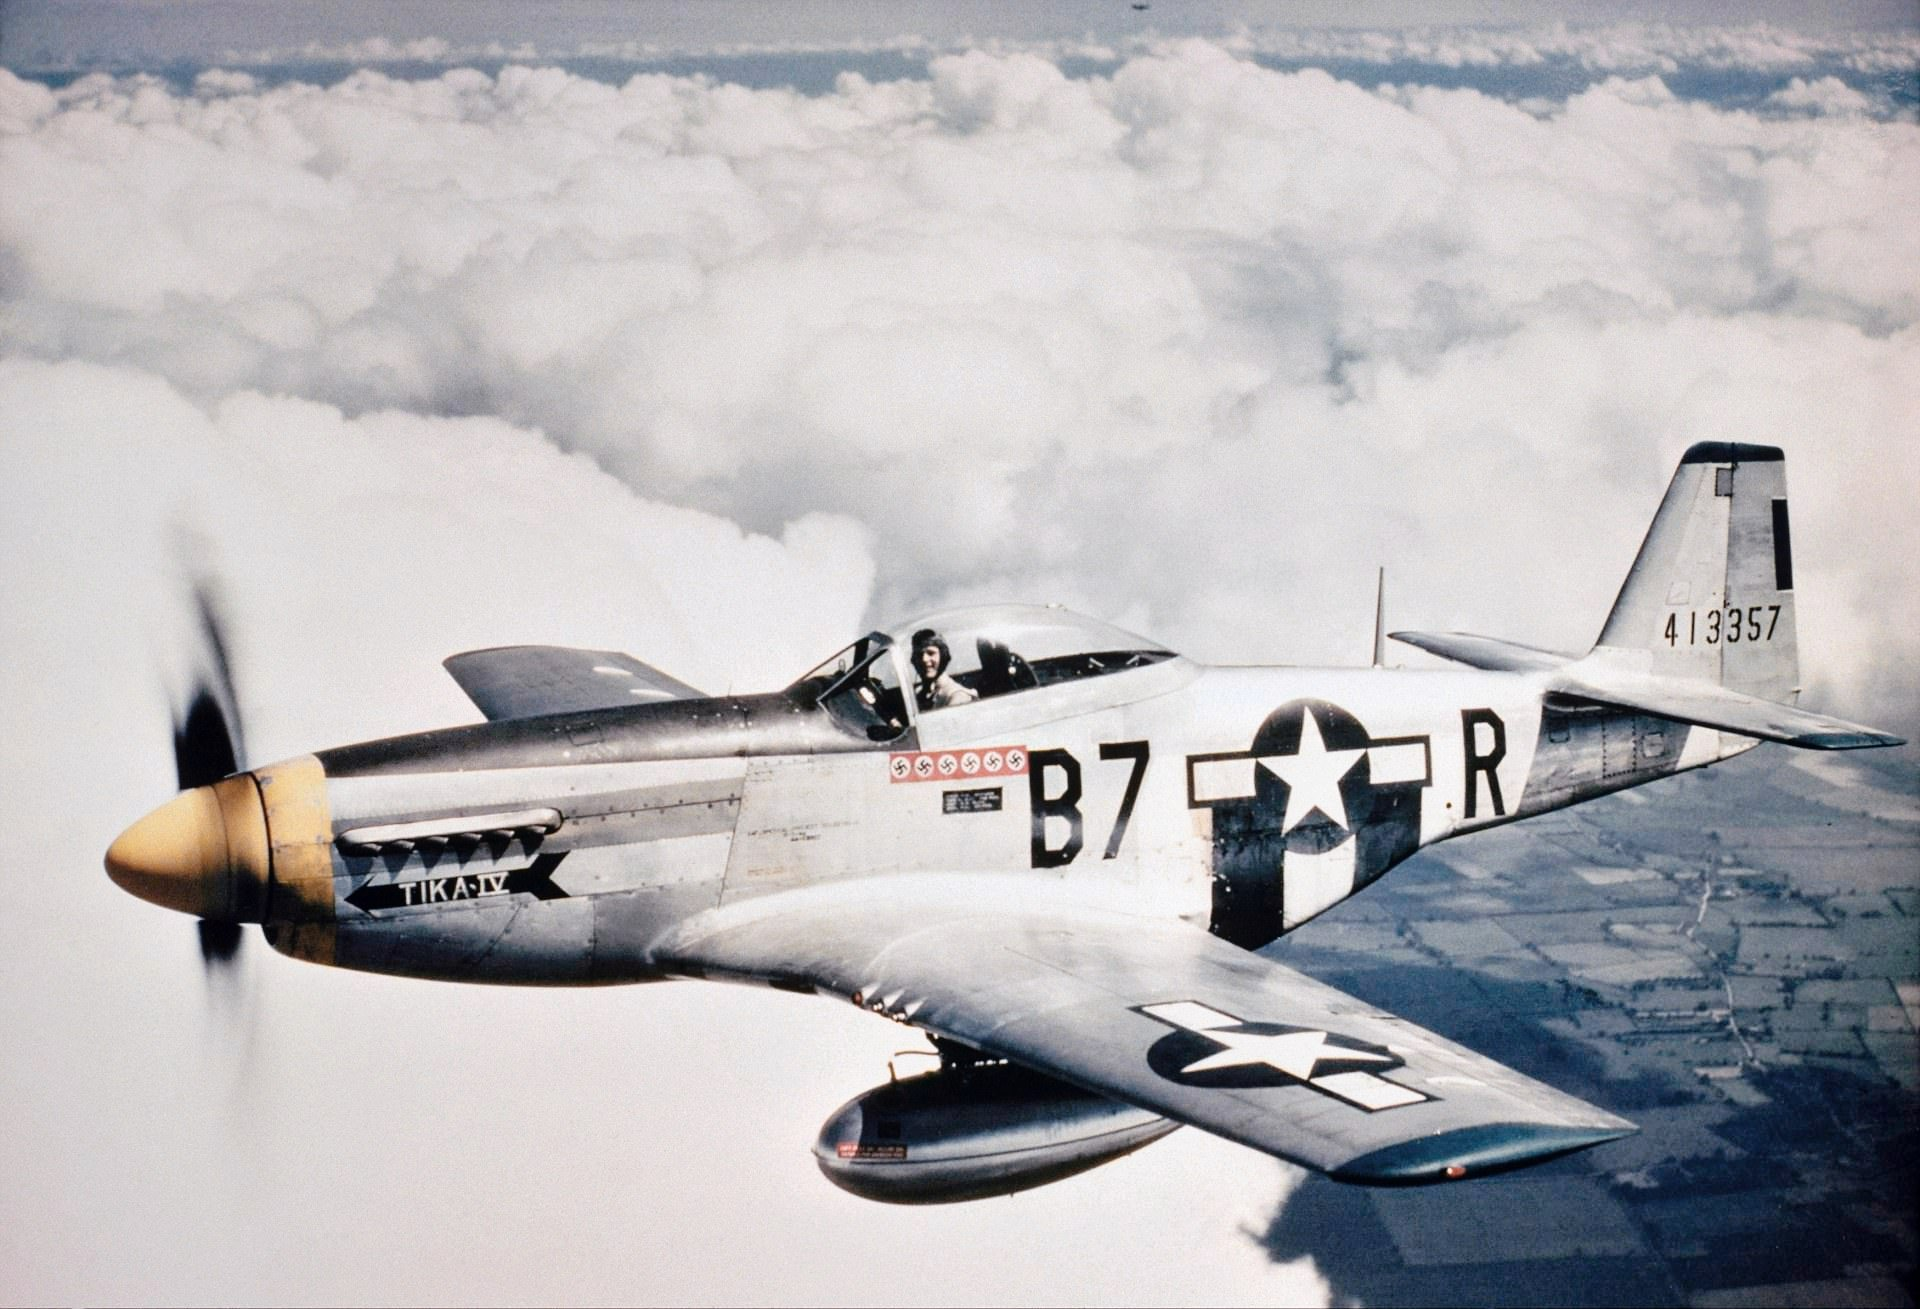
\includegraphics[width=0.90\textwidth]{P-51-mustang}
	\vspace{10pt}
	\caption{North American P-51 Mustang. Image from \cite{wikipedia_mustang}.}
	\label{fig:mustang}
\end{figure}

However it appears that the aeroelasticity problem was not considered from the perspective of natural laminar flow airfoils. This is a surprising fact considering the P-51 Mustang (figure~\ref{fig:mustang}), a fighter aircraft in the Royal Air Force designed in 1940, incorporated a wing with a natural laminar flow airfoil section \citep{green08}. The first aeroelastic study on laminar wings was performed as late as 2011 by \cite{mai11}. This, along with a subsequent investigation by \cite{hebler13}, brought to light a peculiar characteristic of unsteady laminar wings, \textit{i.e.} the presence of non-linearities in the unsteady aerodynamic forces. The classical unsteady aerodynamic theories did not predict non-linear unsteady responses and thus fail to account for such behavior. Inspired by this, \cite{lokattthesis} performed experiments on unsteady NLF airfoils and also found strong non-linearities in the aerodynamic forces. Consistent in the explanation for the non-linearities in all these studies was the role of transition over the wing surface. When transition on the airfoil suction-side was fixed (with a trip) near the leading edge, the non-linearities seemed to disappear. These results indicated a need for a more in-depth study of the evolving boundary layer in such unsteady laminar airfoils. Classical theories negate the role of the boundary layer by invoking the inviscid assumption and it is apparent that such an assumption is no longer be justified for laminar wings. Characteristics of the unsteady boundary layer are the subject of investigation in the present work.

\thesisstructure The thesis is structured as follows:
\begin{itemize}
	\item An overview of the numerical method used for the simulations is given in Chapter 2.
	\item Chapter 3 gives an overview of the numerical simulations performed in the study.
	\item The main conclusions of the current work are given in Chapter 4 along with an outlook for future work.
	\item The next part of the thesis includes the individual papers and internal reports. 
\end{itemize}

%===============================================================================
\chapter{Numerical Method}
%===============================================================================

\section{Numerical Discretization}

The numerical code used for the simulations is Nek5000, which is an open source research code developed by \cite{nek5000} at Argonne National Laboratory. The code solves the incompressible Navier--Stokes equations (\ref{eqn:navier_stokes}) in non-dimensional form:
\begin{subequations}
	\label{eqn:navier_stokes}	
	\begin{eqnarray}
	\frac{\partial u_{i}}{\partial t} + u_{j}\frac{\partial u_{i}}{\partial x_{j}} =  - \frac{1}{\rho}\frac{\partial p}{\partial x_{i}} + \frac{1}{Re}\bigg(\frac{\partial^{2} u_{i}}{\partial x_{j}\partial x_{j}}  \bigg) +f_{i} \\
	\frac{\partial u_{i}}{\partial x_{i}} = 0
	\end{eqnarray}
\end{subequations}
where $x_{i}$ is the coordinate direction, $u_{i}$ is the velocity component, $p$ is the pressure and $Re$ is the defined Reynolds number. The discretization of the Navier--Stokes equations is based on a spectral-element method, first proposed by \cite{patera84}. The method allows the mapping of elements to complex geometries along with a high-order spatial discretization within the elements, thus combining the generality of finite-element methods with the accuracy of spectral methods \citep{patera84}.
The spatial discretization in each element is performed following the $P_{N}$-$P_{N-2}$ \citep{maday89} formulation with velocity represented by high-order Lagrange interpolants through the Gauss--Lobatto--Legendre (GLL) quadrature points, while the pressure is represented on the staggered Gauss-Legendre (GL) quadrature points. The nonlinear terms are treated explicitly by third-order extrapolation (EXT3), while the viscous terms are treated implicitly by a third-order backward differentiation scheme (BDF3). Over-integration is used for the removal of aliasing errors. Nek5000 is written in Fortran 77 and C with efficient scaling for up to 1 million MPI ranks \citep{fischer15}.

%%%%%%%%%%%%%%%%%%%%%%%%%%%%%%%%%%%%%%%%%%%%%%%%%%%%%%%%%%%%%%%%%%%%%%
\section{Relaxation-term large-eddy simulation (RT-LES)}

Owing to the high Reynolds numbers and large time-scales of integration for some of the flow cases, a direct numerical simulation (DNS), which requires a resolution of all the spatial scales of the flow, leads to prohibitively high computational costs. In recent years a technique of wall-resolved large-eddy simulations has emerged as a computationally cheaper alternative to DNS, while also exhibiting the high-fidelity characteristics of DNS.
The technique has been utilized in the studies of spatially developing boundary layers \citep{eitel14}, pipe flows \citep{chin15} and flow over wings \citep{uzun10,lombard15}. The success of the approach has motivated its use in the present work. The wall-resolved LES method used is based on the RT3D variant of the ADM-RT approach first used by \cite{schlatter04}. The method has been shown to be reliable in accurately predicting transition and also preserving the characteristic structures which are seen in the DNS of transitional flows by \cite{schlatter06}. This particular quality of the LES model is crucial since there is a large focus on the unsteady transition in the present work. The LES method supplements the governing equations with a dissipative term $-\chi\mathcal{H}(u)$. The equations of motion for the resolved velocity and pressure thus read as
\begin{subequations}
	\label{eqn:rt_les}	
	\begin{eqnarray}
	\frac{\partial u_{i}}{\partial t} + u_{j}\frac{\partial u_{i}}{\partial x_{j}} =  - \frac{1}{\rho}\frac{\partial p}{\partial x_{i}} + \frac{1}{Re}\bigg(\frac{\partial^{2} u_{i}}{\partial x_{j}\partial x_{j}}  \bigg) + f_{i} -\chi\mathcal{H}(u_{i}), \\
	\frac{\partial u_{i}}{\partial x_{i}} = 0,
	\end{eqnarray}
\end{subequations}	
where $\mathcal{H}$ is a defined high-pass spectral filter and $\chi$ is a model parameter which together with $\mathcal{H}$ determines the strength of the dissipative term. The high-pass filter function $\mathcal{H}$ is defined such that the resultant relaxation-term only has energy in the highest modes, defined by a cut-off mode-number $N_{c}$. Figure~\ref{fig:filter_shape} illustrates the shape of the filter function in spectral space.
\begin{figure}[h]
	\centering
	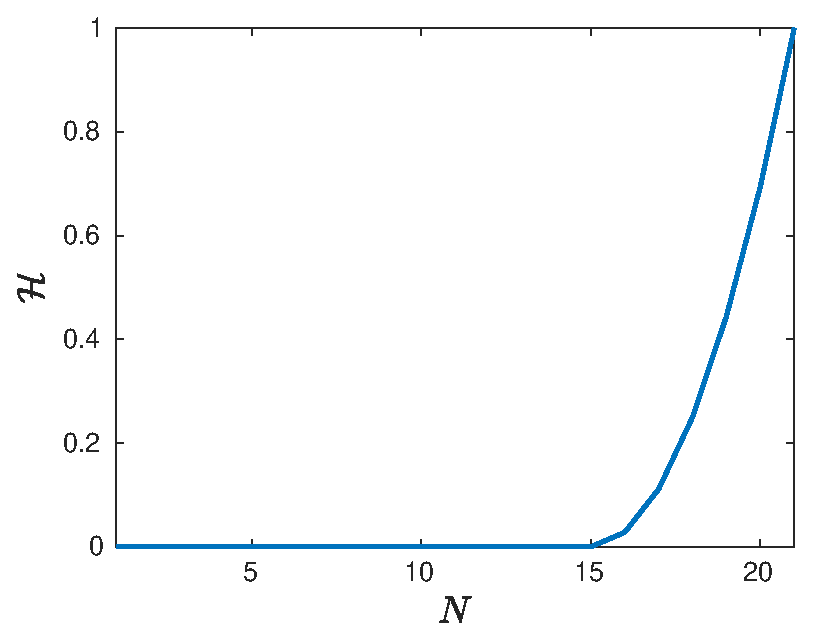
\includegraphics[width=0.60\textwidth]{filter_shape}
	\caption{Transfer function for the spectral coefficients for the filter $\mathcal{H}$ with number of modes $N=21$ and cut-off mode number $N_{c}=16$.}
	\label{fig:filter_shape}
\end{figure}

Several parameter optimization studies were performed to determine the optimum value of $\chi$ and filter shape $\mathcal{H}$ using turbulent channel flow simulations. The LES results were compared with the DNS database of \cite{moser99} and the optimum parameters were further validated for a flow around a wing section at $Re_{c}=400,000$. A good agreement was found between the LES and the DNS data of \cite{hosseini16}, and the optimized parameters were then used for all subsequent simulations.

\section{Arbitrary-Lagrangian-Eulerian (ALE)}

Typical solutions of unsteady fluid flows utilize the Eulerian framework where the coordinate system is fixed in space. A fixed coordinate system however becomes infeasible when the domain boundaries are in motion, as is the case of fluid-structure interaction problems, or when there is a free surface which may lead to a deforming interface. An appropriate method is needed to account or the motion of the boundaries and/or the interior grid points. One such method which substantially simplifies the difficulties arising out of moving boundaries is the Arbitrary-Lagrangian-Eulerian (ALE) method. The method was proposed in a finite-difference framework by \cite{hirt74} and later brought to the spectral-element framework by \cite{ho90,ho91}. The technique combines both the Lagrangian and Eulerian formulations such that, the Navier--Stokes may be solved with the grid points moving with the fluid elements \textit{i.e.} in a Lagrangian framework, or with fixed grid points (Eulerian), or with grid points moving in an arbitrary prescribed manner. The heart of the technique lies in the formulation of the total time rate of change of a quantity in the ALE frame, defined analogously to the material derivative. Thus for a quantity $\mathbf{F(x_{i},t)}$, the change due to small increments $dx_{i}$ and $dt$ may be expressed as \citep{kundu02}
\begin{align}
	dF = \frac{\partial F}{\partial t}dt + \frac{\partial F}{\partial x_{i}}dx_{i}.
	\label{eqn:material_deriv_df}
\end{align}
One may choose to follow any arbitrary path along which this quantity is evaluated, in which case the quantities $dx_{i}$ and $dt$ are related by the velocity of the (grid) point along this arbitrary path $w_{i} = dx_{i}/dt$. The relation results in the expression referred to as the ALE derivative \citep{deville02}, here denoted as $\delta F/\delta t$ to differentiate it from the very similar expression for the material derivative (which is evaluated along the fluid particle trajectory)
\begin{align}
\frac{\delta F}{\delta t} = \frac{\partial F}{\partial t} + w_{i}\frac{\partial F}{\partial x_{i}}.
\label{eqn:ale_derivative}
\end{align}
When $w_{i}$ is equal to the fluid velocity $u_{i}$, we recover the familiar Lagrangian expression for the material derivative $DF/Dt$. On the other hand, when $w_{i}=0$, we get the local (Eulerian) rate of change of the quantity $F$. The material derivative and the ALE derivative share a simple relationship defined using a relative velocity of the fluid particle with respect to the grid motion $c_{i} = u_{i} - w_{i}$, which may be used in the definition of material derivative to obtain
%\begin{subequations}
	\begin{align}
%	\frac{DF}{Dt} = \frac{\partial F}{\partial t} + u_{i}\frac{\partial F}{\partial x_{i}} \nonumber\\
%	\frac{DF}{Dt} = \bigg(\frac{\partial F}{\partial t} + w_{i}\frac{\partial F}{\partial x_{i}}\bigg) + c_{i}\frac{\partial F}{\partial x_{i}} \nonumber \\	
	\frac{DF}{Dt} = \frac{\delta F}{\delta t} + c_{i}\frac{\partial F}{\partial x_{i}}.
	\label{eqn:ale_material_derivative}
	\end{align}
%\end{subequations}
Thus the Navier--Stokes in the ALE formulation may be expressed as 
\begin{subequations}
	\label{eqn:ale_navier_stokes}	
	\begin{align}
	\frac{\delta u_{i}}{\delta t} + (u_{j} - w_{j})\frac{\partial u_{i}}{\partial x_{j}} =  - \frac{1}{\rho}\frac{\partial p}{\partial x_{i}} + \frac{1}{Re}\bigg(\frac{\partial^{2} u_{i}}{\partial x_{j}\partial x_{j}}  \bigg) +f_{i}, \\
	\frac{\partial u_{i}}{\partial x_{i}} = 0,
	\end{align}
\end{subequations}
where $w_{j}$ is the velocity of the grid points. The solution of the Navier--Stokes is then a simple matter of evaluating a suitable grid velocity. 

In many cases, such as the flow over an oscillating airfoil, the velocity of the grid points at the boundary (airfoil surface) may be explicitly known. \cite{ho90,ho91} propose to extend this velocity to the interior points of the domain by solving an elliptic problem for the mesh velocity. In the present work we take a simpler approach to prescribing the mesh velocities in the interior domain. Recognizing the simple trigonometric form of a harmonic pitching motion, all mesh points may simply be prescribed a solid body rotation with the instantaneous angular velocity of the airfoil. However a pure solid-body rotation would also displace the domain boundaries. Therefore a damping function is used to smoothly reduce the rotational velocity away from the airfoil boundary such that the mesh motion is zero at the far-field, inlet and outflow boundaries. Thus for an airfoil with an instantaneous rotation rate of $\Omega_{z}(t)$, the mesh velocity is prescribed as:
\begin{align}
	w_{i}(x,y,z,t) = \underbrace{(\Omega_{z}(t) \times \vec{R})}_{\text{Solid body rotation}} \overbrace{f(|\ \vec{r}\ |)}^{Damping}
	\label{eqn:mesh_velocity}
\end{align}
where $\vec{r}$ is the normal distance of a grid point from the airfoil surface, $\vec{R}$ is the distance from the rotational axis and $f(r)$ is a damping function which can be prescribed in many different ways, depending on one's preferences. The damping function needs to have two essential properties, \textit{i.e.} it must be equal to 1 when $|\vec{r}|=0$, which implies the mesh points at the airfoil boundary move with the surface (solid body rotation at the airfoil surface), and it must smoothly decay to zero close to the far-field boundaries, which allows the external boundaries of the computational domain to remain fixed in physical space. Figure~\ref{fig:mesh_rotation_damping} shows the damping function used in the present work as a function of the normal distance from the airfoil surface.
\begin{figure}[h]
	\centering
	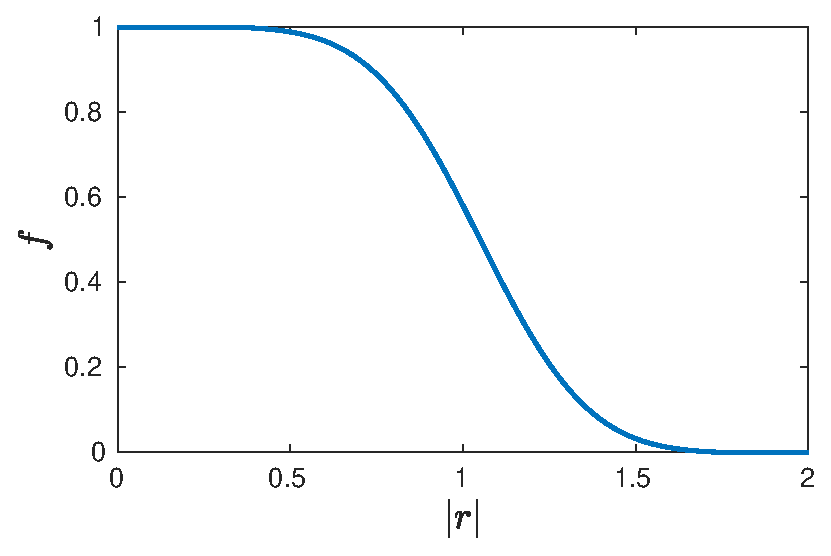
\includegraphics[width=0.55\textwidth]{damping_func}
	\vspace{5pt}
	\caption{Damping function $f(r)$ for the mesh velocities.}
	\label{fig:mesh_rotation_damping}
\end{figure}
The damping function moves the grid points close to the airfoil surface with the same rotational velocity of the airfoil and spreads out the mesh deformation into the interior of the domain. This damping function is calculated once at the beginning of the simulation. Hence all quantities $\Omega_{z}(t),\ \vec{r},\ f(r)$ which are needed for prescribing the mesh velocity are explicitly known at each time-step without the need for solving an elliptic equation as in \cite{ho90,ho91}. 

\section{Free-stream turbulence}

Isotropic, homogeneous free-stream turbulence is prescribed at the inlet and far-field boundaries to add small disturbances to the flow-field, which simulate the disturbances found in a wind-tunnel or in free-flight conditions. The free-stream turbulence is prescribed as a superposition of Fourier modes with a random phase shift. The maximum and minimum amplitudes of the wavenumber vector are prescribed quantities and are limited by the resolution of the spatial discretization and size of the domain respectively. The wavenumber space between the minimum and the maximum is divided into 20 concentric shells with each shell representing the amplitude of the three-dimensional wavenumber vectors lying on the shell. 20 points are randomly chosen on each shell with the location of each point representing the three-dimensional components of the wavenumber vector. Thus the free-stream turbulence is represented by a total of 400 fourier modes. Care is taken to avoid very small wavenumber components which result in wavelengths in physical space that are larger than the computational domain. The streamwise length scales are transformed to a temporal frequency by invoking Taylor's frozen turbulence hypothesis and using the local mean streamwise velocity at the inlet for the space-time conversion. The amplitude of the free-stream modes on each spherical shell is scaled using the von K\'arm\'an spectrum. Figure~\ref{fig:fst_duct} shows an instantaneous visualization of the streamwise velocities in a doubly-periodic duct flow case with high ($5\%$) free-stream turbulence intensity prescribed at the the inlet. Figure~\ref{fig:ti_decay} shows the spatial decay of turbulence intensity. After a small initial distance of adjustment from the inlet, the turbulence intensity decays as a power law. A very similar method for generating free-stream turbulence for simulations of flat-plate boundary layers is used by \cite{schlatterdiploma,brandt04,schlatter08} and more recently for wind turbine simulations by \cite{kleusberglicenciate}.

\begin{figure}[h]
	\centering
	\begin{subfigure}[t]{0.49\textwidth}
		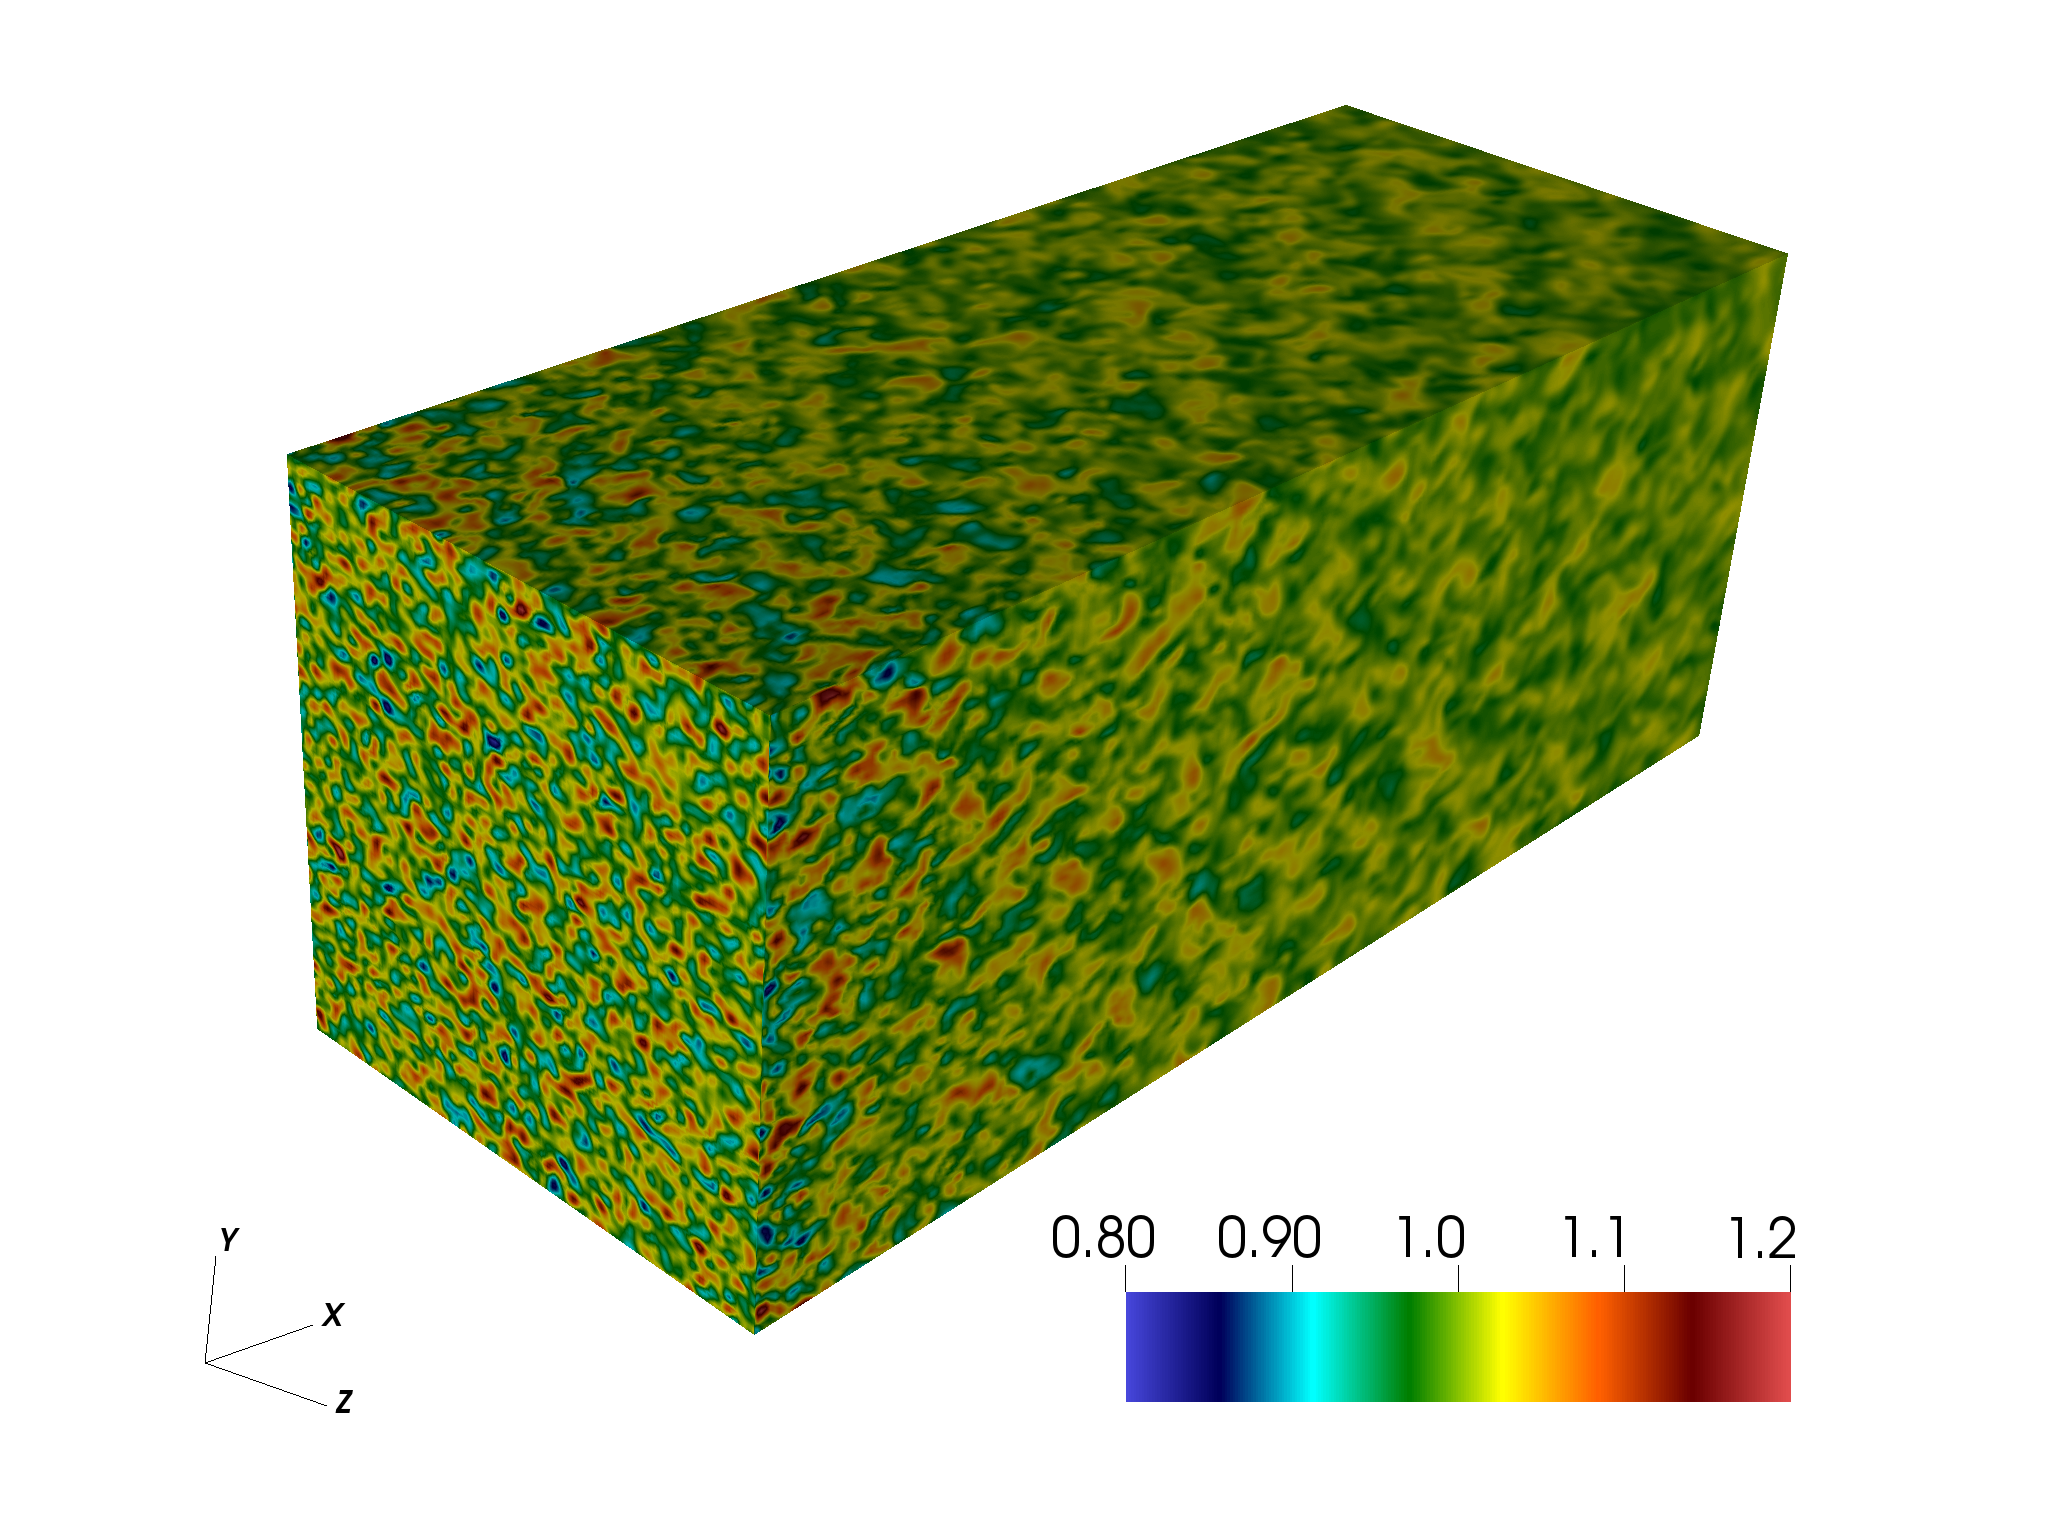
\includegraphics[width=1\textwidth]{fst_duct_vx0000.png}
		\caption{Visualization of free-stream turbulence prescribed at the inlet for a doubly periodic duct flow. Colors represent the instantaneous streamwise velocity.}
		\label{fig:fst_duct}
	\end{subfigure}
	\begin{subfigure}[t]{0.49\textwidth}
		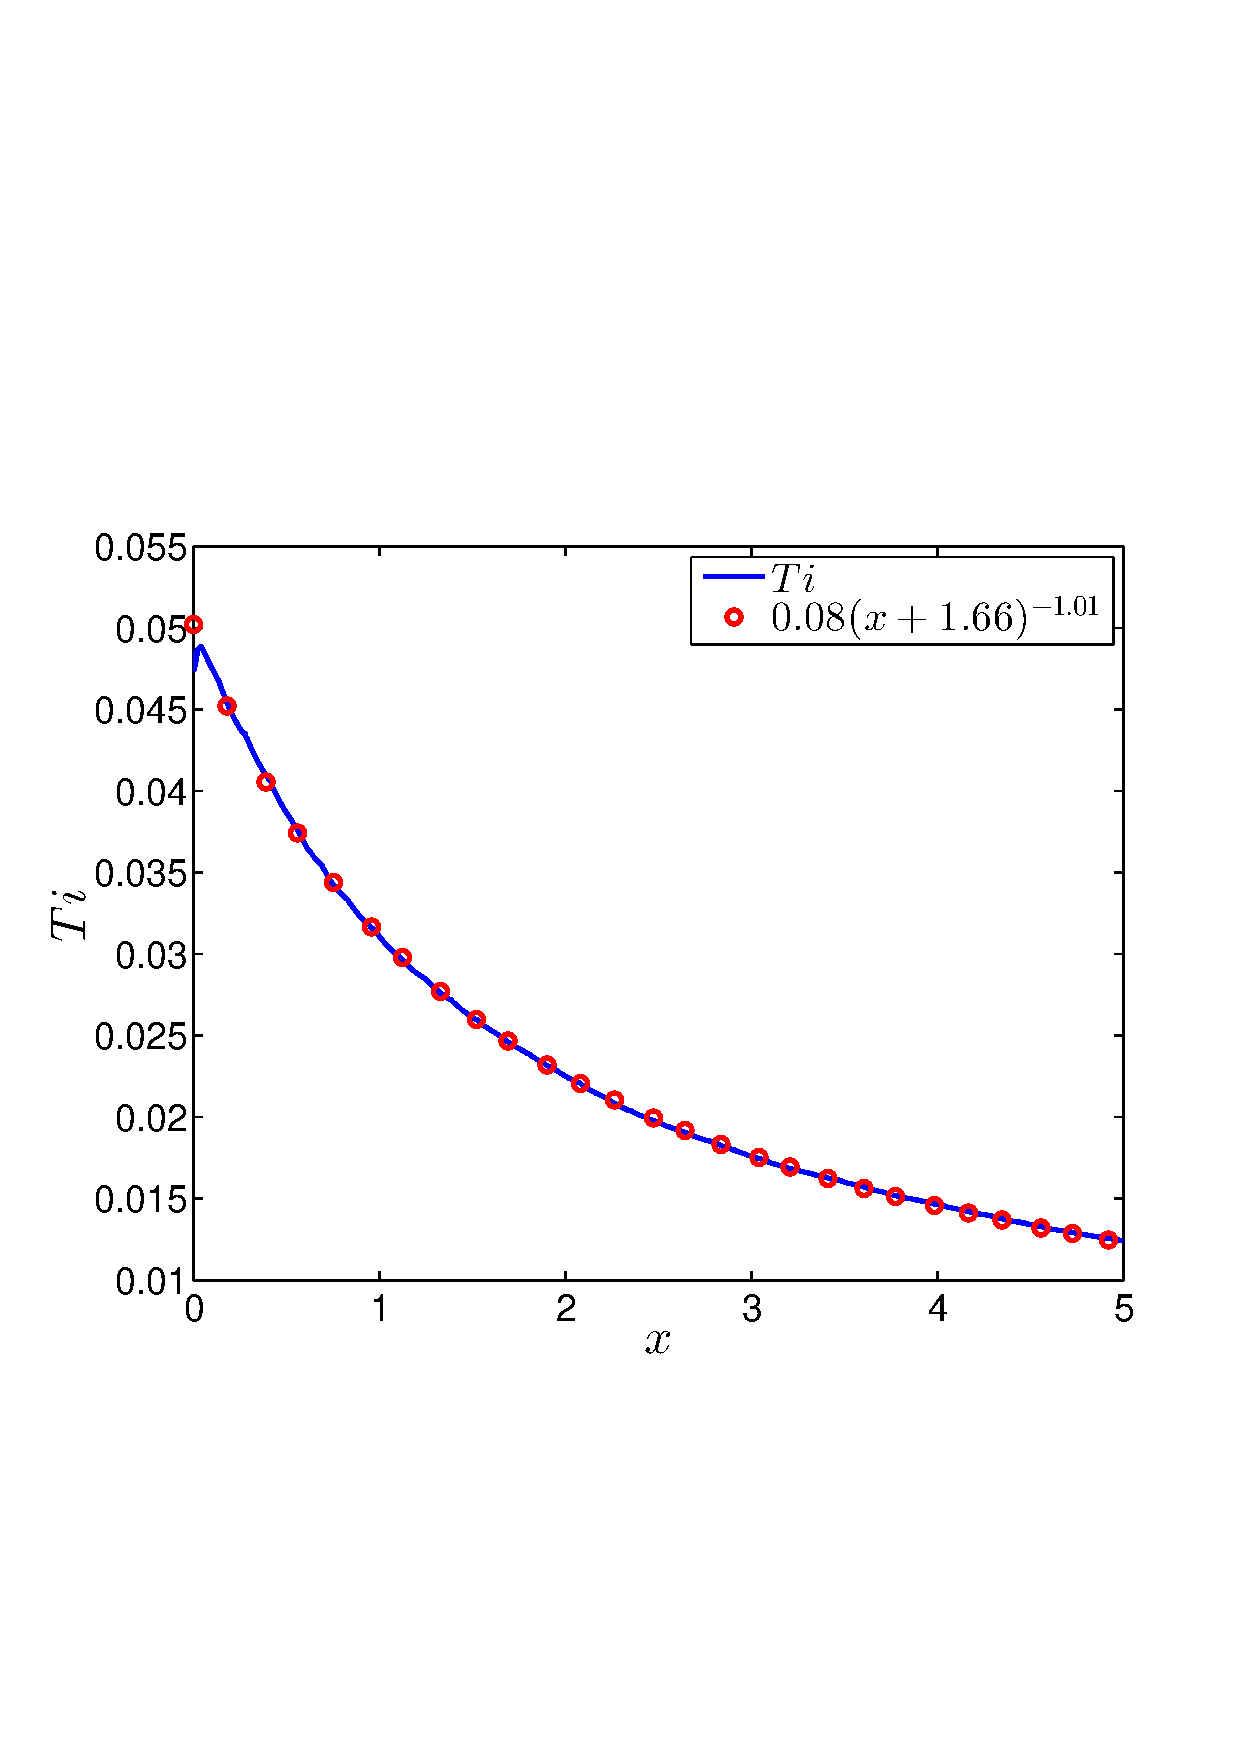
\includegraphics[width=1\textwidth]{ti_decay}
		\caption{Decay of turbulence intensity with streamwise distance, along with the least-squares fit of a power law.}
		\label{fig:ti_decay}
	\end{subfigure}
\end{figure}

%===============================================================================
\chapter{Overview of numerical simulations}
%===============================================================================

\section{Flow around unsteady wings}

The unsteady experiments of \cite{mai11,hebler13} and \cite{lokattthesis} have shown that aerodynamic non-linearities are related to the movement of transition over the suction side of the airfoil. Thus unsteady boundary layer dynamics play an important role in aerodynamic response of NLF airfoils. The present work investigates the unsteady boundary layers with a particular focus on unsteady transition with the aim to shed light on the phenomenon of non-linear unsteady aerodynamic response. The airfoil used in the investigation is the ED36F128 (with a $13.8^{\circ}$ flap deflection), designed at the Aeronautical and Vehicle Engineering department at KTH. It is a natural laminar flow airfoil, which has been used in several steady and unsteady experiments \citep{lokatt17,lokattthesis}. The unsteady experiments have shown the non-linearities that appear to be typical of laminar airfoils \citep{lokattthesis}. The results of the steady and unsteady experiments using this airfoil have been made available to us by Dr. Eller and Dr. Lokatt. Non-linearities in the unsteady aerodynamic forces are observed for only a certain range of angle of attack $\alpha$. Therefore a careful assessment of the data was needed in order to select the right parameter range where the relevant flow physics could be observed in the numerical simulations. The data in the experimental campaign was gathered primarily through pressure taps located around airfoil for the calculation of unsteady aerodynamic forces. Thus measurements of the unsteady boundary layer characteristics was not available through the experimental data. Calculations using an integral boundary layer code XFOIL \citep{drela89}, were used to complement the experimental data and better evaluate the state of the boundary layer in the static measurements.

Figure~\ref{fig:tr_xfoil_100_750} shows the calculated transition locations for two different Reynolds numbers ($Re_{c}=100,000$ and $Re_{c}=750,000$) using XFOIL and figure~\ref{fig:765k_static_cz_foil} shows the experimentally measured normal force coefficient as well as calculations from XFOIL for $Re_{c}=750,000$. For the higher Reynolds number case, transition location varies sharply with angle of attack within the range $3.4^{\circ}<\alpha<6.5^{\circ}$. Aerodynamic non-linearities can also be observed approximately within the same angle of attack range (figure~\ref{fig:765k_static_cz_foil}). For the lower Reynolds number case, no experimental data is available. Therefore solely XFOIL calculations are used and the parameter range is selected where the transition location varies rapidly with angle of attack. This is found for an angle of attack range of $6.7^{\circ}<\alpha<8.0^{\circ}$.
\begin{figure}[!h]
	\centering
	\begin{subfigure}[t]{0.45\textwidth}
		\caption{}
		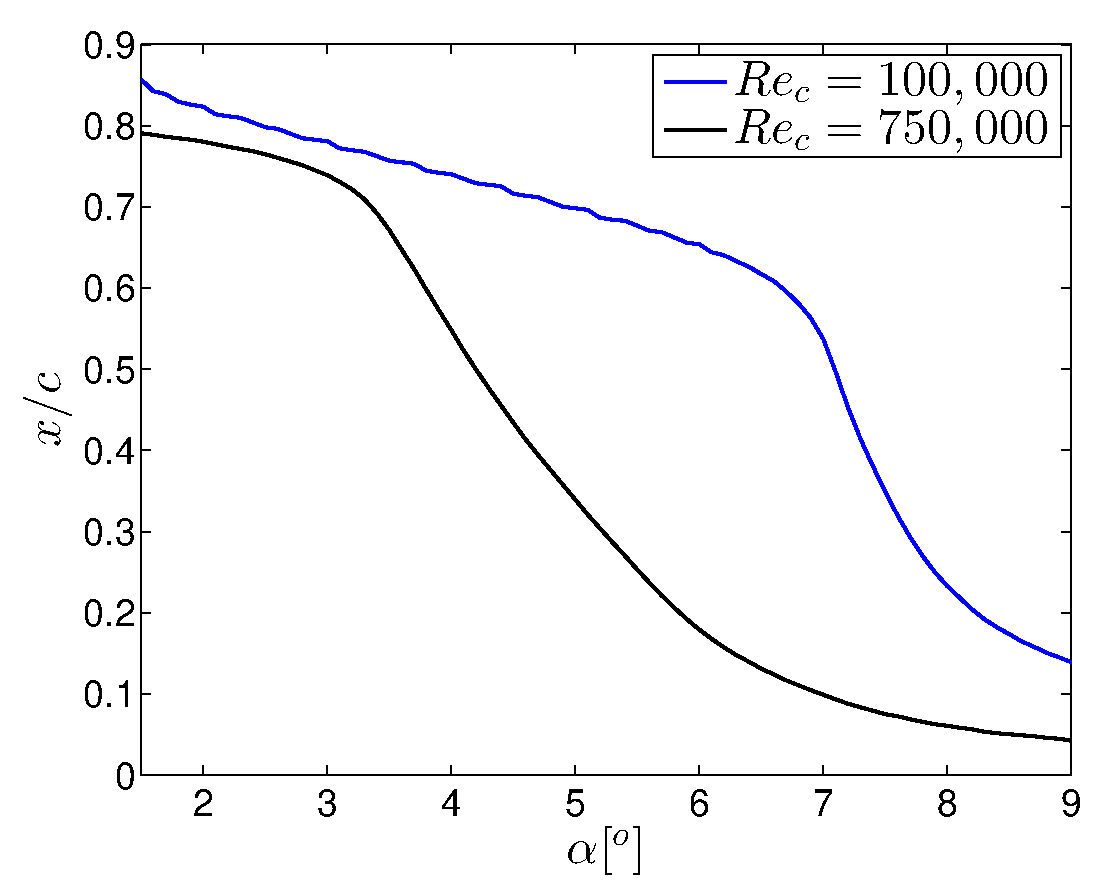
\includegraphics[width=1\textwidth]{tr_xfoil_100_750}
		\label{fig:tr_xfoil_100_750}		
	\end{subfigure}
	\begin{subfigure}[t]{0.45\textwidth}
		\caption{}
		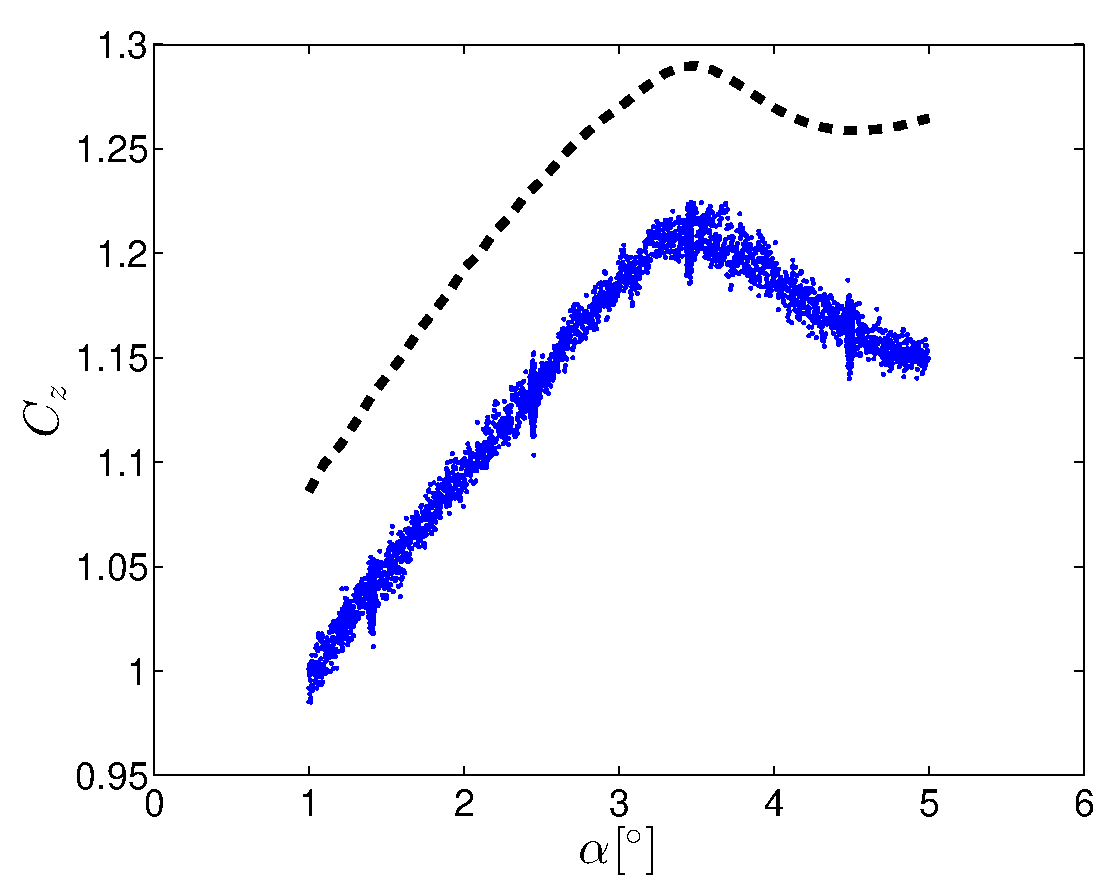
\includegraphics[width=1\textwidth]{765k_static_model_cz_xfoil}
		\label{fig:765k_static_cz_foil}
	\end{subfigure}
	\caption{(a) Transition location calculated using XFOIL for two different Reynolds numbers. (b) Normal force coefficient measured in experiments (dots) and from XFOIL calculations (dashed line) for $Re_{c}=750,000$.}		
\end{figure}
Numerical simulations are performed with stationary airfoils to ensure the expected static boundary layer characteristics are captured by the numerical simulations.  Figure~\ref{fig:overview_la2_750k_stationary} depicts the instantaneous vortical structures in the flow for $Re_{c}=750,000$ for an angle of attack $\alpha=2.4^{\circ}$ and $\alpha=4.4^{\circ}$ which shows the change in boundary layer characteristics in the static cases. Similarly, figure~\ref{fig:overview_isocontour_aoa} shows the static boundary layer characteristics for $Re_{c}=100,000$ at $\alpha=6.7^{\circ}$ and $\alpha=8.0^{\circ}$.
\begin{figure}[h]
	\centering
	\begin{subfigure}[t]{0.49\textwidth}
		\caption{$\alpha=2.4^{\circ}$}		
		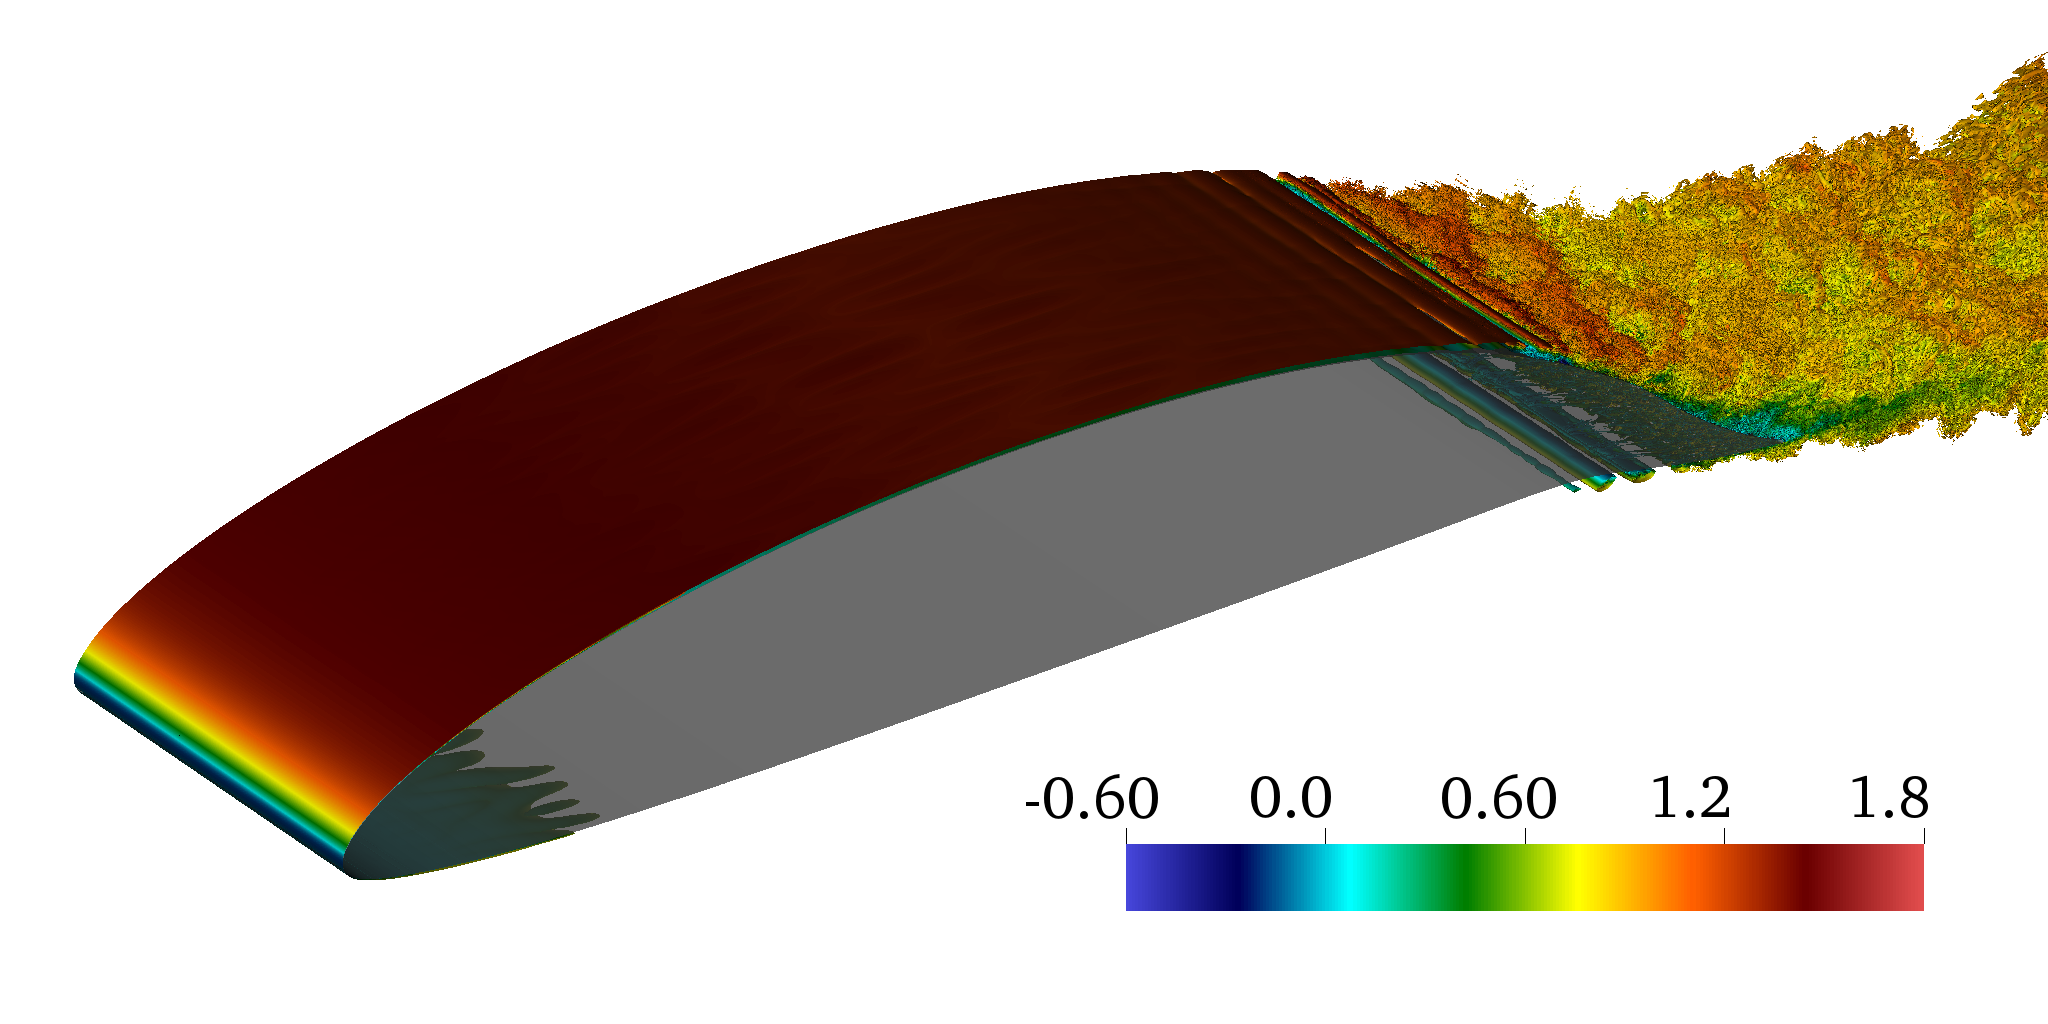
\includegraphics[width=1\textwidth]{paper2/imgs2/pitch_re750k0001}
		\label{fig:overview_la2_aoa24}
	\end{subfigure}
	\begin{subfigure}[t]{0.49\textwidth}
		\caption{$\alpha=4.4^{\circ}$}		
		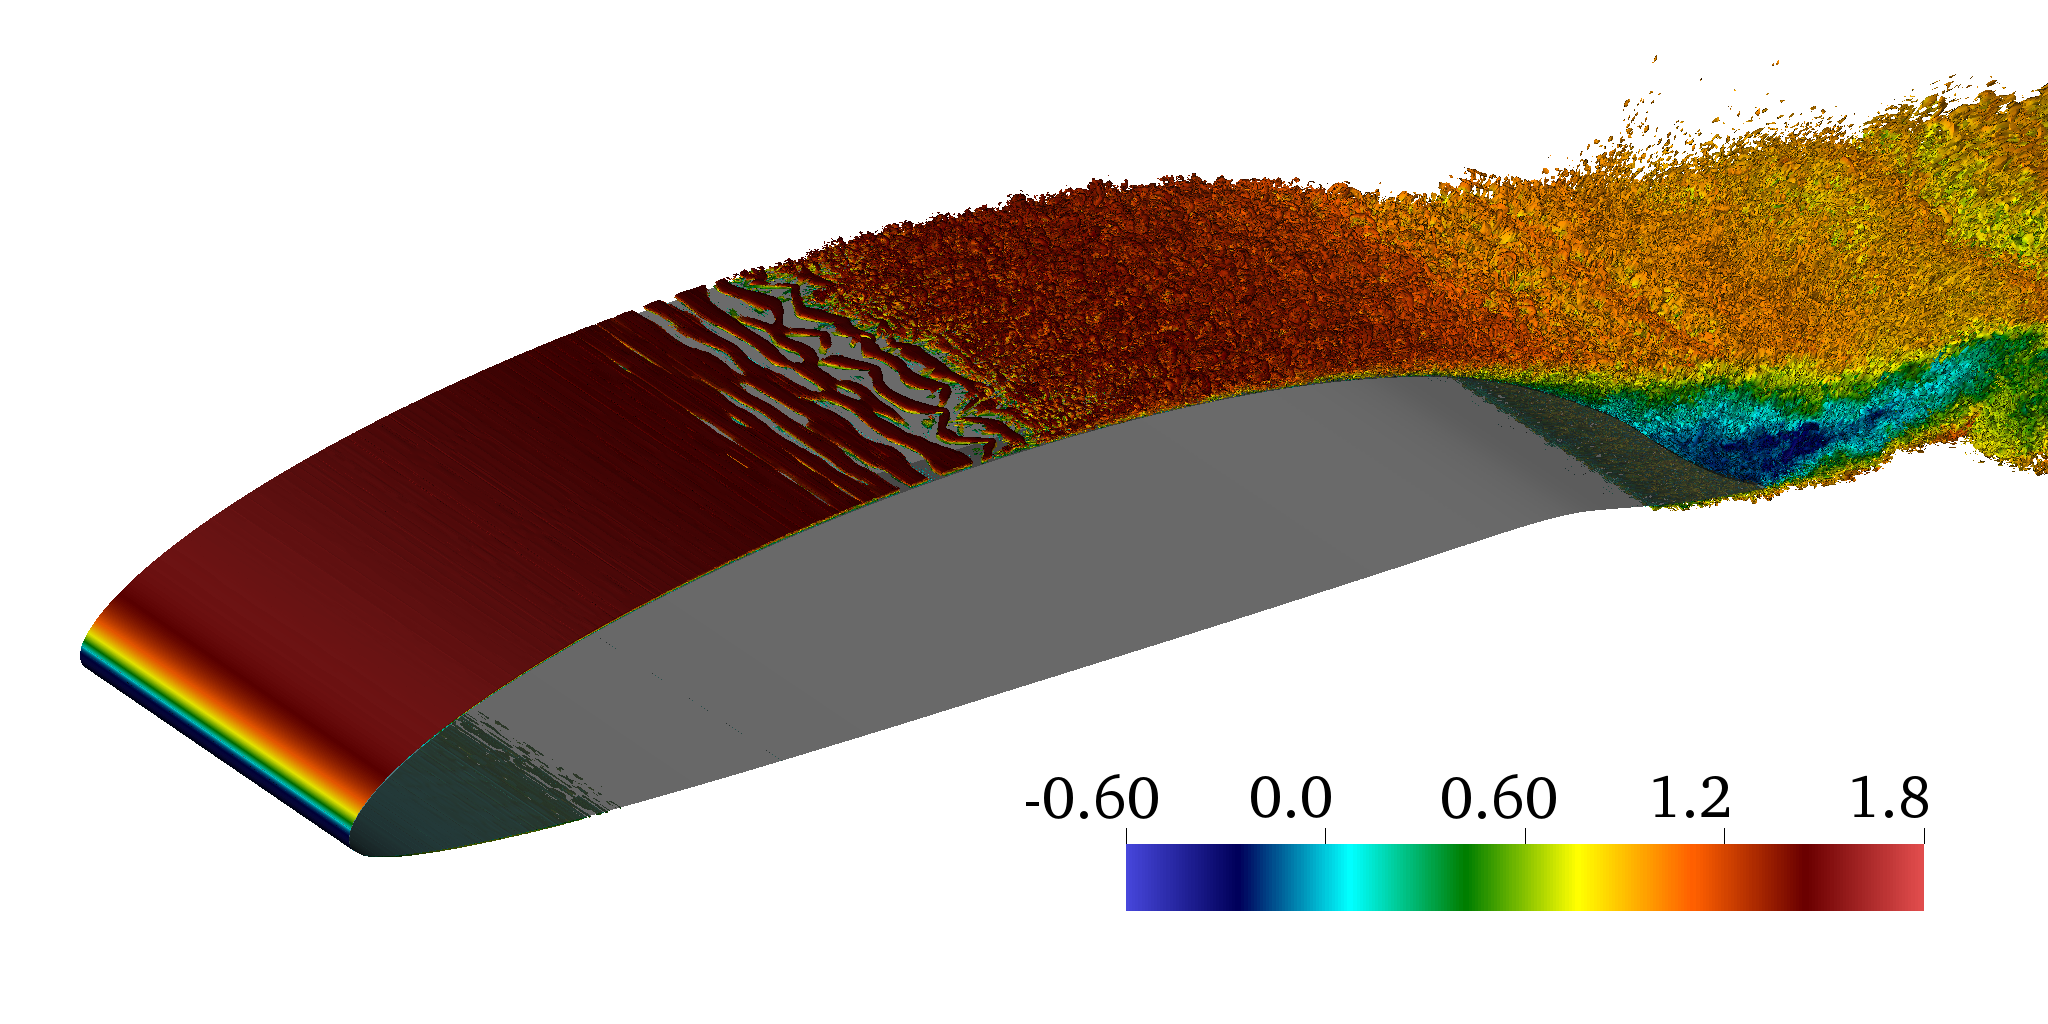
\includegraphics[width=1\textwidth]{paper2/imgs2/pitch_re750k0002}
		\label{fig:overview_la2_aoa44}		
	\end{subfigure}	
	\caption{Instantaneous vortical structures identified by the $\lambda_{2}$ criterion for the two stationary angle of attack simulations at $Re_{c}=750,000$.}
	\label{fig:overview_la2_750k_stationary}
\end{figure}

\begin{figure}[t]
	\begin{subfigure}[b]{0.49\textwidth}
		\centering
		\caption{$\alpha=6.7^{\circ}$}		
		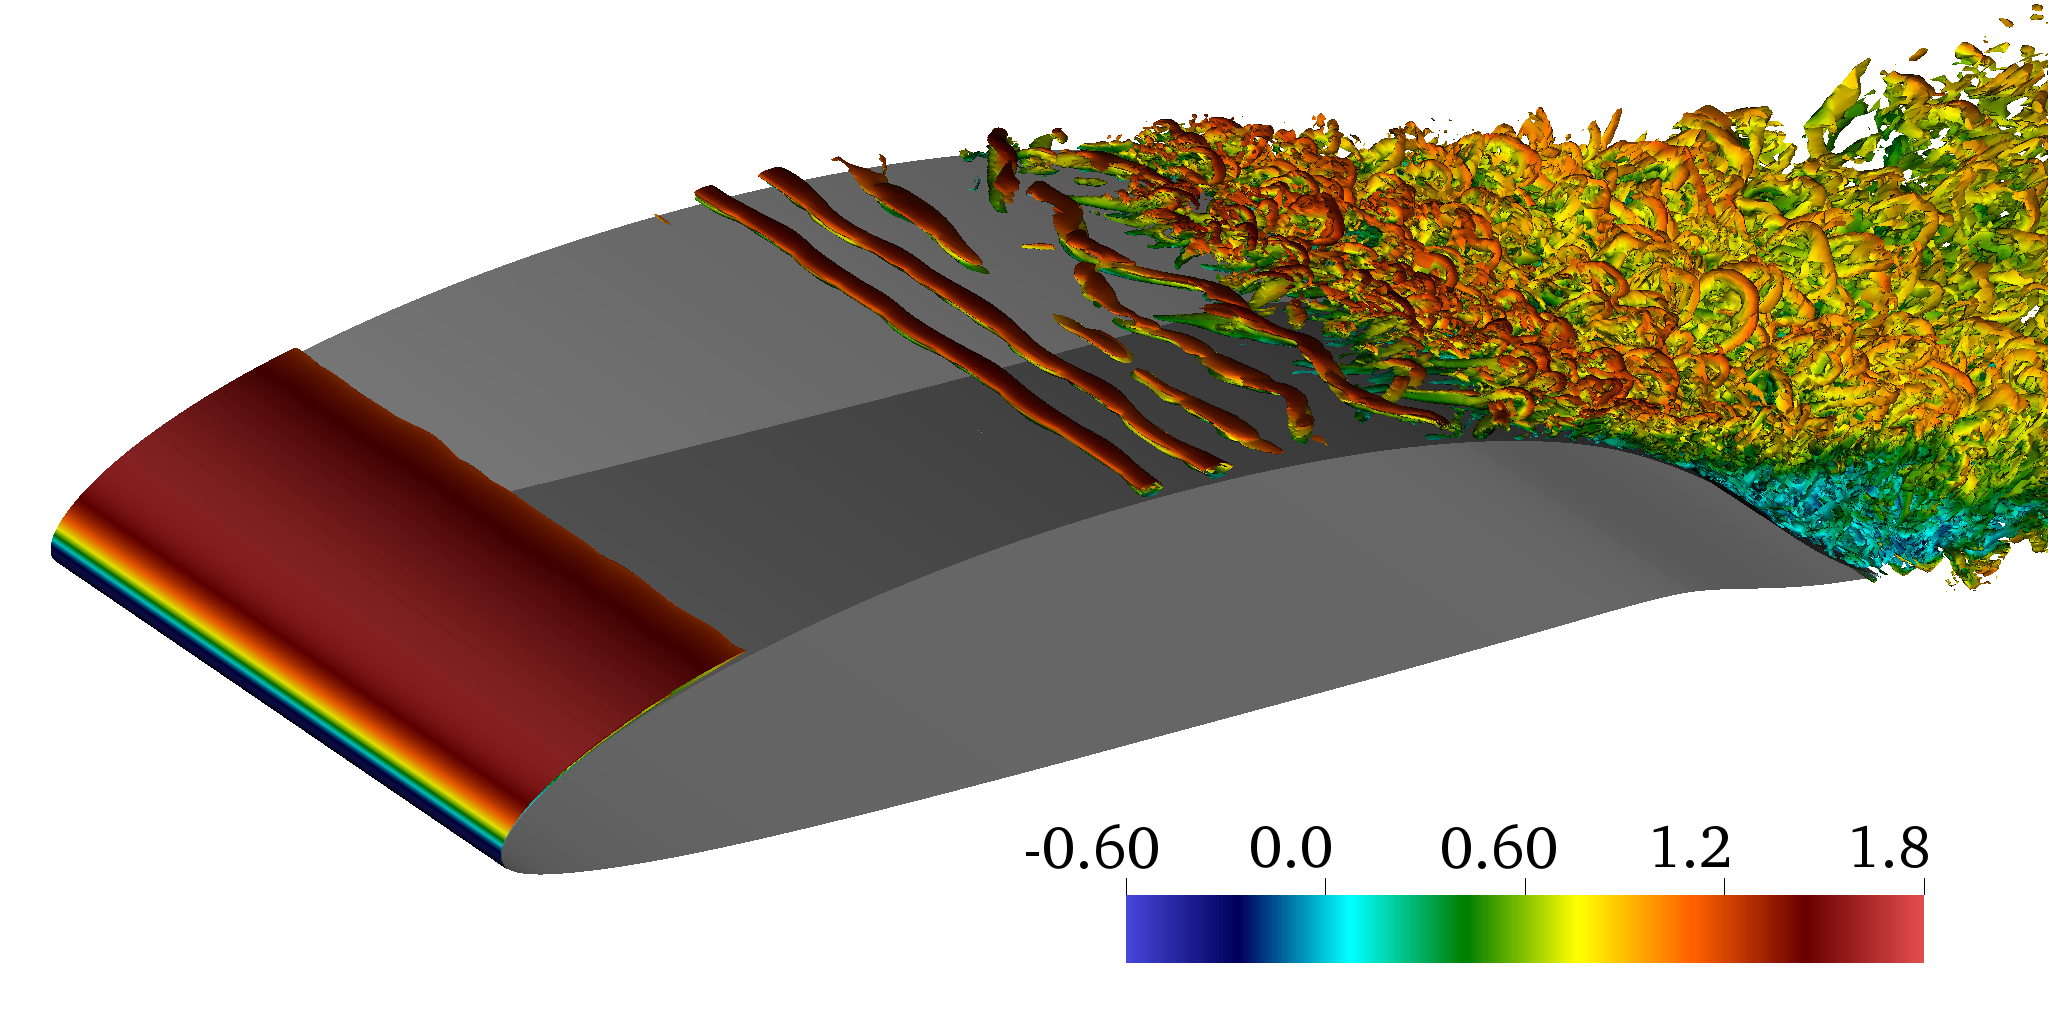
\includegraphics[width=1\textwidth]{paper3/imgs/re100k_static67_0001}
		\label{fig:overview_aoa67_iso}
	\end{subfigure}
	\begin{subfigure}[b]{0.49\textwidth}
		\centering
		\caption{$\alpha=8.0^{\circ}$}		
		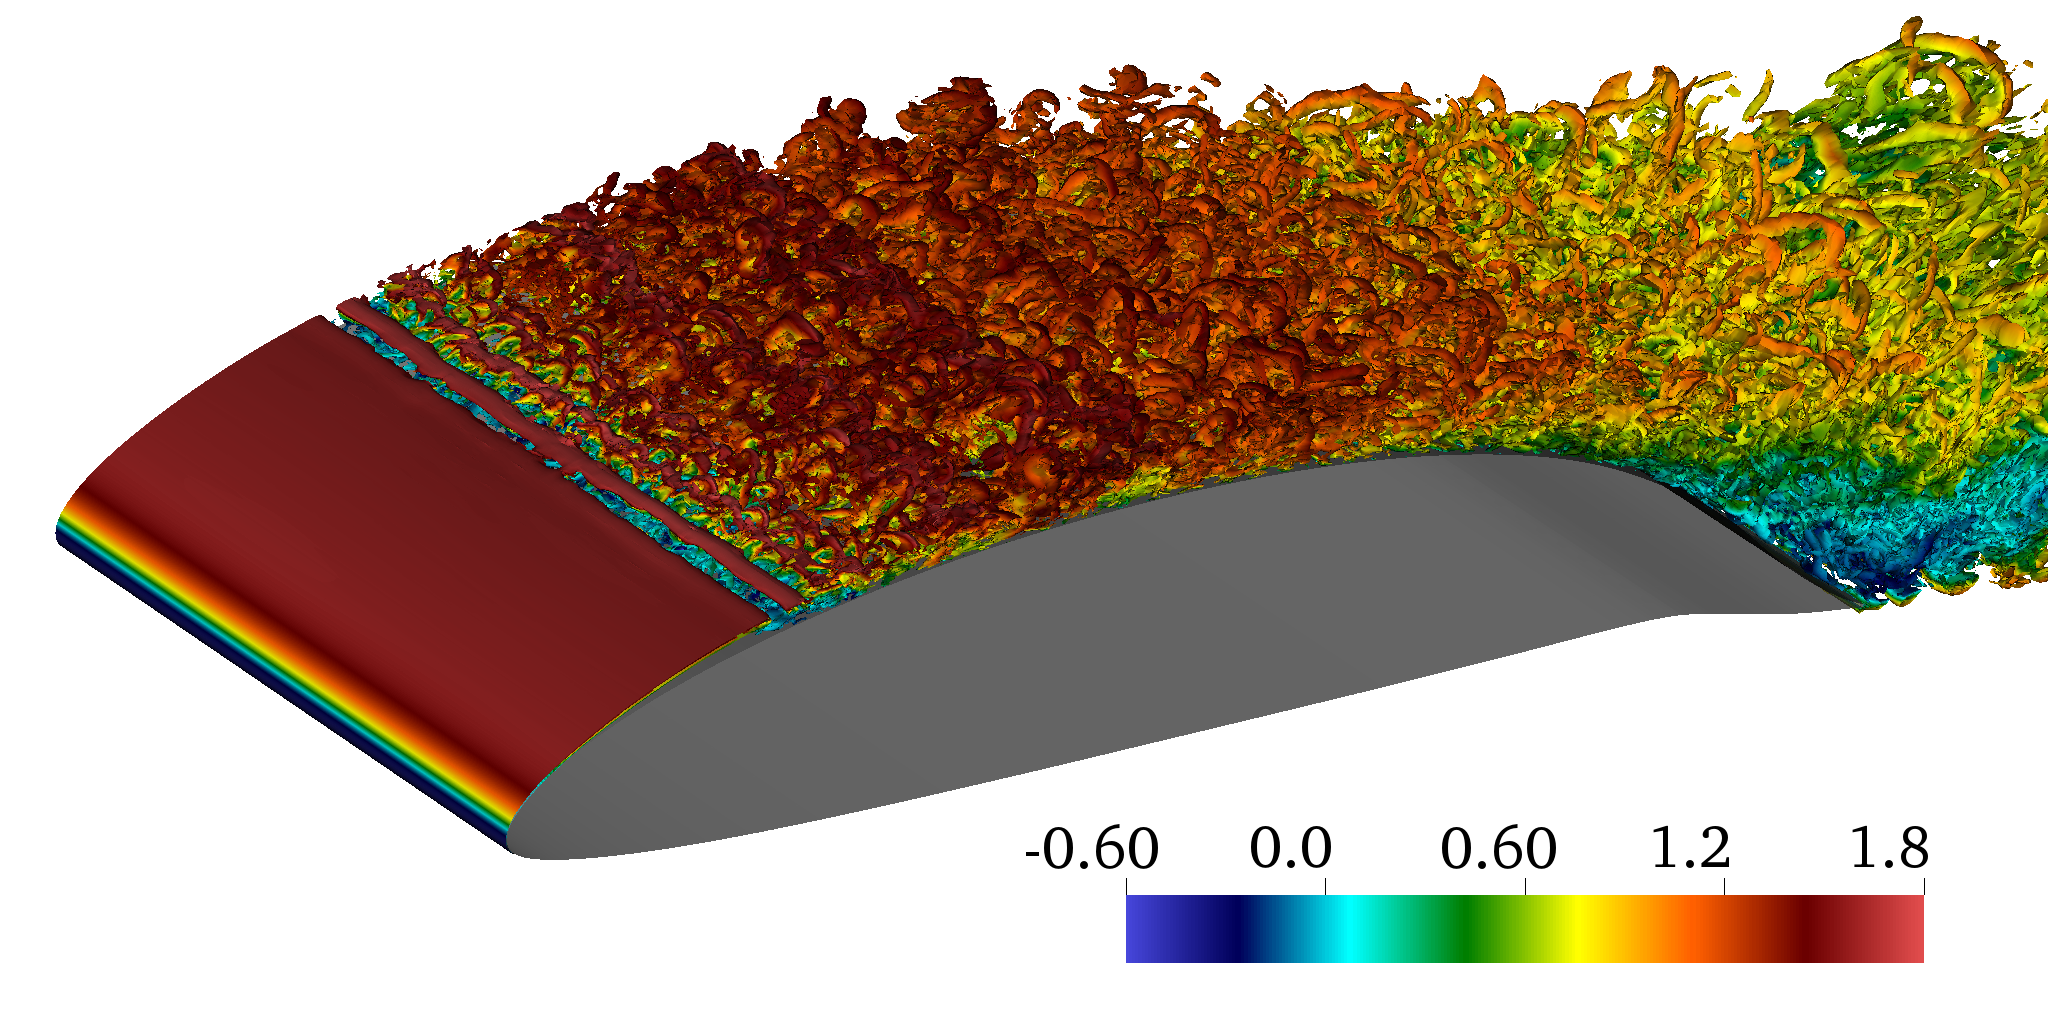
\includegraphics[width=1\textwidth]{paper3/imgs/re100k_static80_0001}
		\label{fig:overview_aoa80_iso}
	\end{subfigure}
	\caption{Isocontours of instantaneous $\lambda_{2}$ structures observed for two different (stationary) angles of attack at $Re_{c}=100,000$.}
	\label{fig:overview_isocontour_aoa}
\end{figure}

For both the Reynolds number cases, significant temporal variation of transition location is also found for the unsteady cases. Figure~\ref{fig:overview_transition_alpha} shows the variation of transition with respect to $\alpha$. The transition locations were calculated using thresholds on the instantaneous spanwise-averaged Reynolds stress $\overline{u'v'}$ and spanwise fluctuation intensity $\overline{w'w'}$. For the lower Reynolds number case the boundary layer also develops a leading-edge laminar separation bubble during the pitch cycle which significantly influences the boundary-layer dynamics.

\begin{figure}[t]
	\begin{subfigure}[b]{0.49\textwidth}
		\centering		
		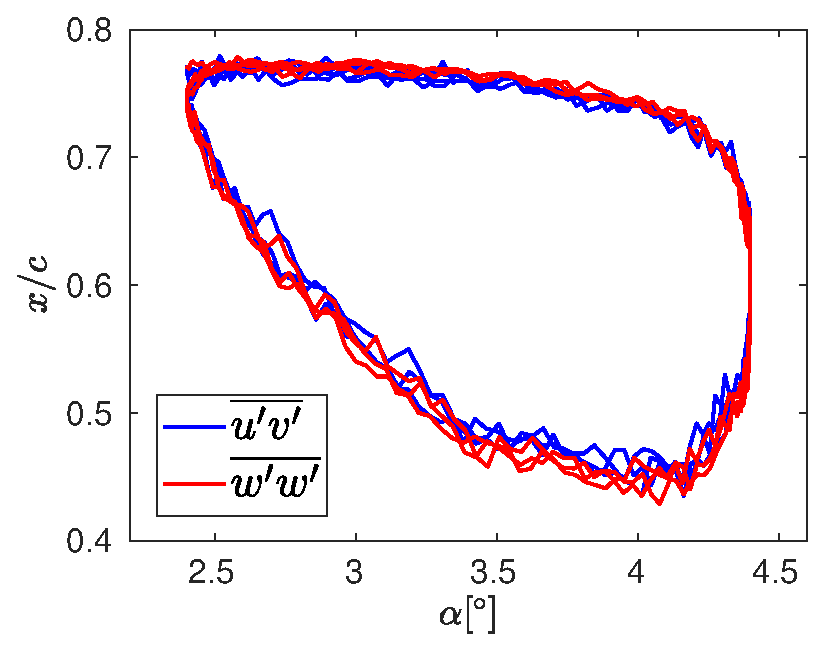
\includegraphics[width=1\textwidth,height=0.80\textwidth]{imgs/750k_transition_alpha.eps}
	\end{subfigure}
	\begin{subfigure}[b]{0.49\textwidth}
		\centering	
		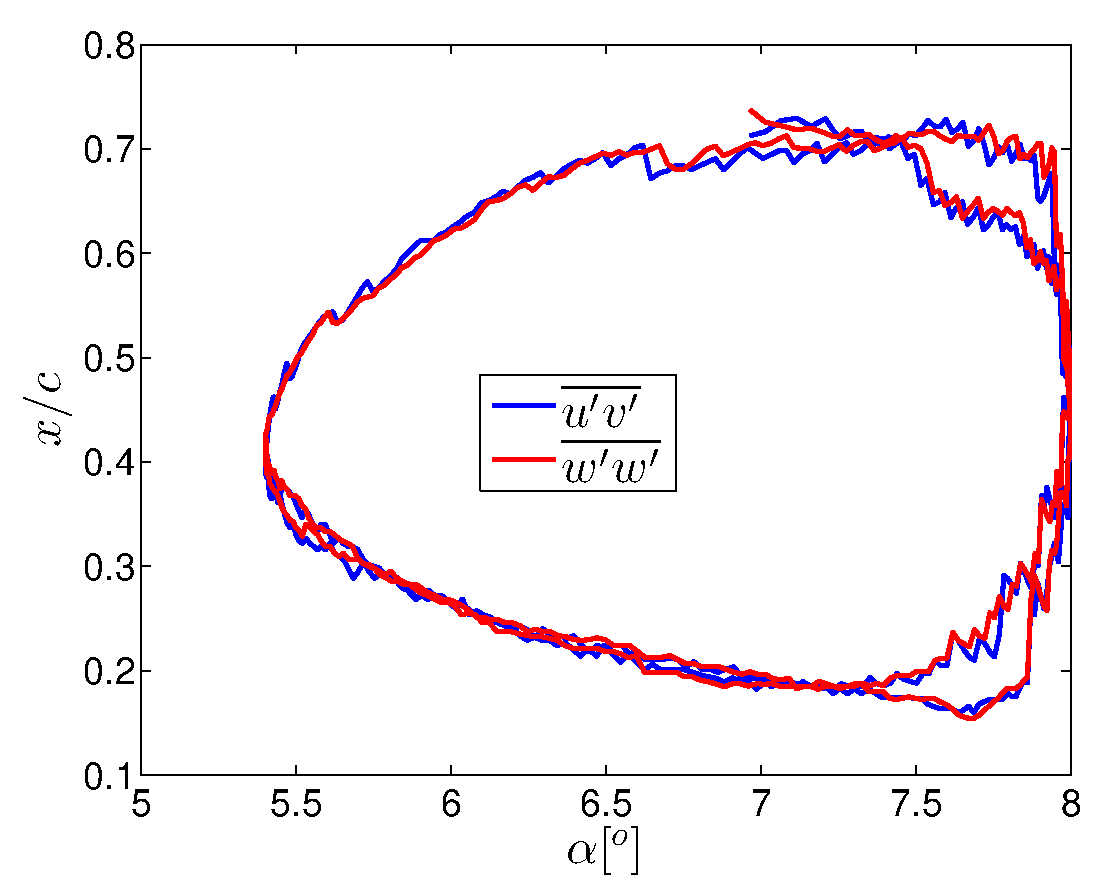
\includegraphics[width=1\textwidth]{paper3/imgs/transition_alpha.eps}
	\end{subfigure}
	\caption{Phase portraits of transition location for (left) $Re_{c}=750,000$ and (right) $Re_{c}=100,000$.}
	\label{fig:overview_transition_alpha}
\end{figure}


\section{Flow around a stationary wing section}

The final paper in the thesis deals with the study of the boundary layer over a wing section at a chord-based Reynolds number of $Re_{c}=1,000,000$. The airfoil used for the study is the asymmetric NACA 4412. A DNS database for the flow around the same airfoil at $Re_{c}=400,000$ is available and comparisons are made between the two cases to assess the effects of changing Reynolds number on the developing boundary layer. The numerical setup is done in a manner very similar to the computational study by \cite{hosseini16}. Figure~\ref{fig:overview_flow_field_re1000k} shows a section of the numerical grid and the instantaneous vortical structures in the flow field. Figure~\ref{fig:overview_beta_Reth_Ret} shows a comparison of the different measures of the boundary layer over the chord-wise distance for the two different Reynolds numbers. While both wall-shear stress (indicated by $Re_{\tau}$) and boundary layer thickness (measured with momentum thickness Reynolds number $Re_{\theta}$) change between the two cases, the Clauser parameter stays nearly the same throughout the chord. This allows comparisons across different Renolds numbers without ambiguity since the pressure gradient histories remain the same with changing Reynolds numbers. 
\begin{figure}[t]
	\centering
	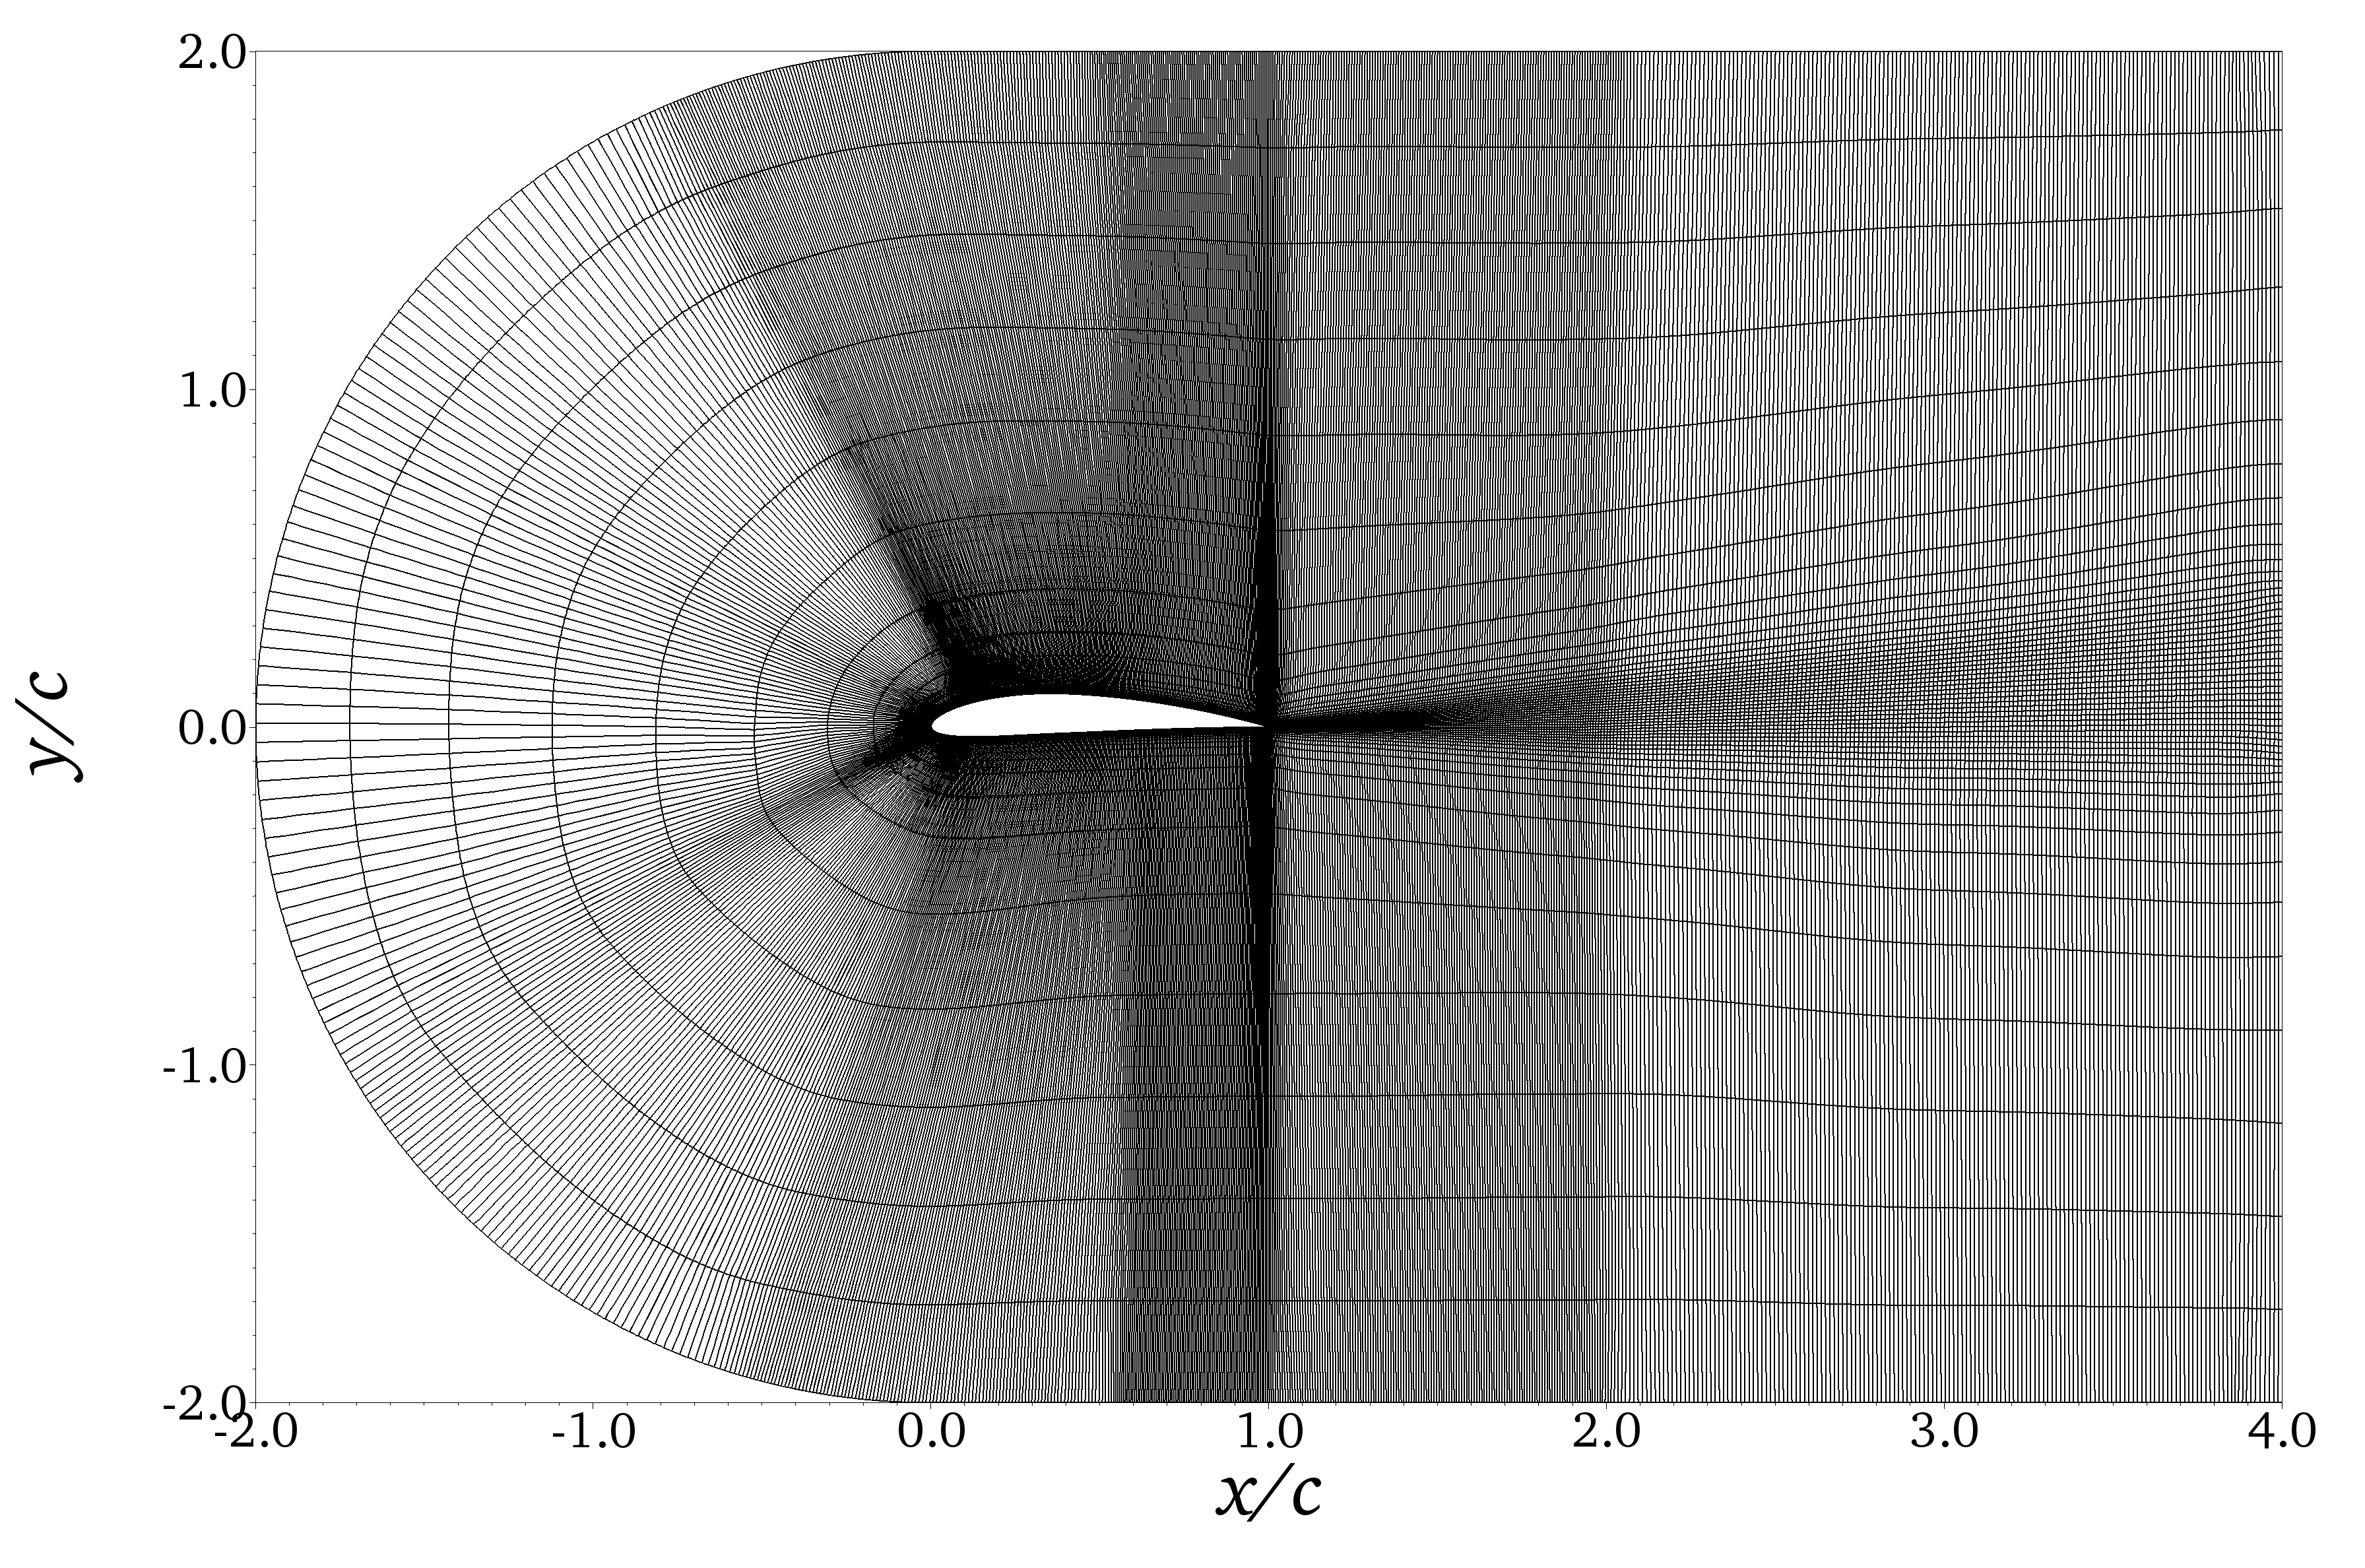
\includegraphics[width=0.49\textwidth]{paper4/imgs/wing_mesh}
	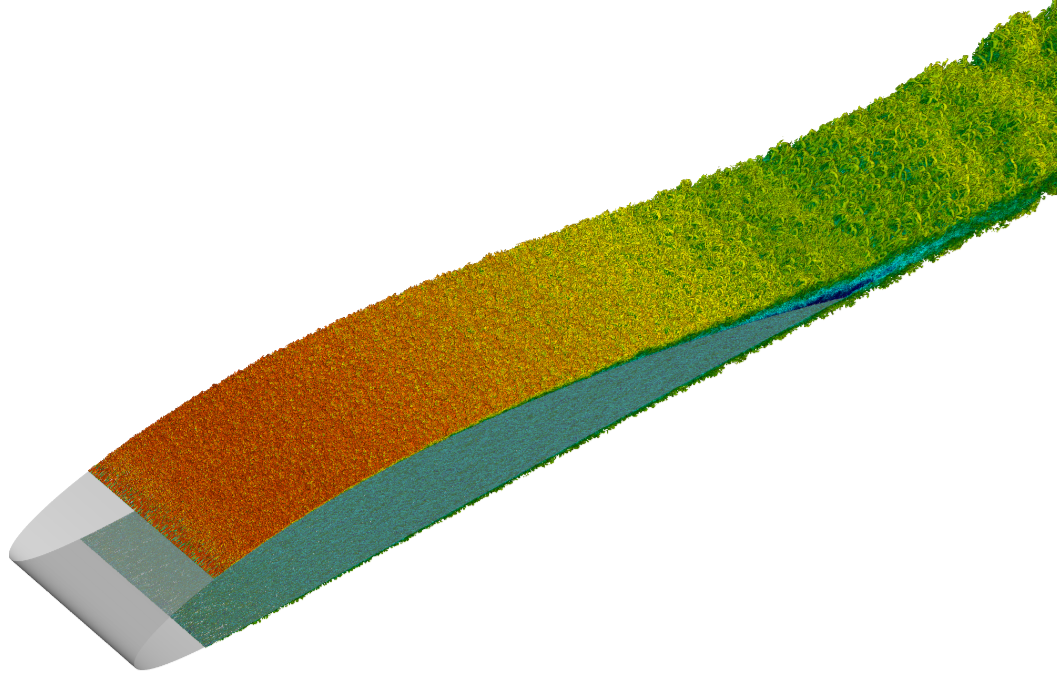
\includegraphics[width=0.49\textwidth]{paper4/imgs/wing_visualization}
	\caption{(Left) Two-dimensional slice of the computational domain showing the spectral-element distribution. (Right) Instantaneous flow field showing coherent structures identified with the $\lambda_{2}$ method \citep{jeong95}, and colored with horizontal velocity. In this figure, dark blue represents a horizontal velocity of $-0.1$ and dark red a value of $2$.}
	\label{fig:overview_flow_field_re1000k}
\end{figure}

\begin{figure}[t]
	\centering
	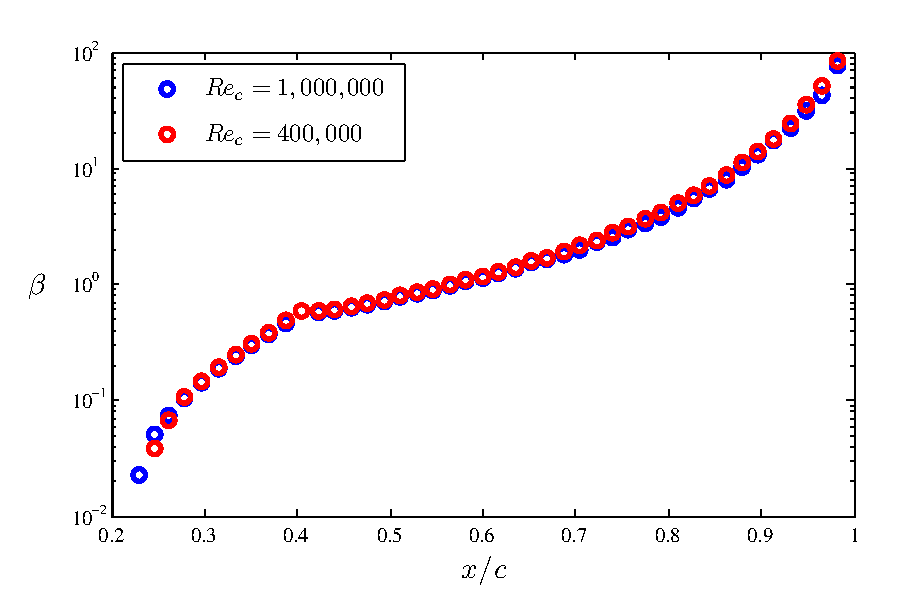
\includegraphics[width=0.49\textwidth]{paper4/imgs/beta_vs_x}
	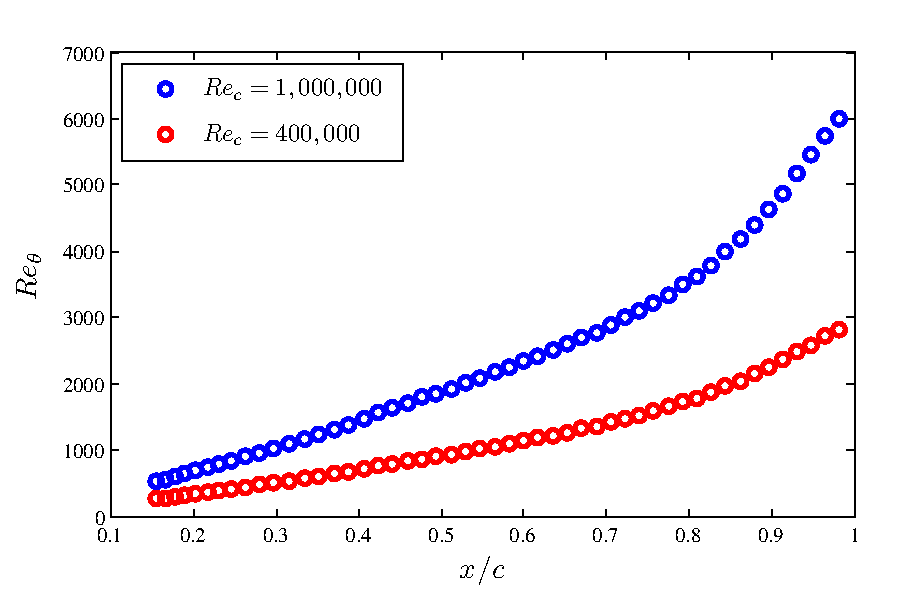
\includegraphics[width=0.49\textwidth]{paper4/imgs/Reth_vs_x}
	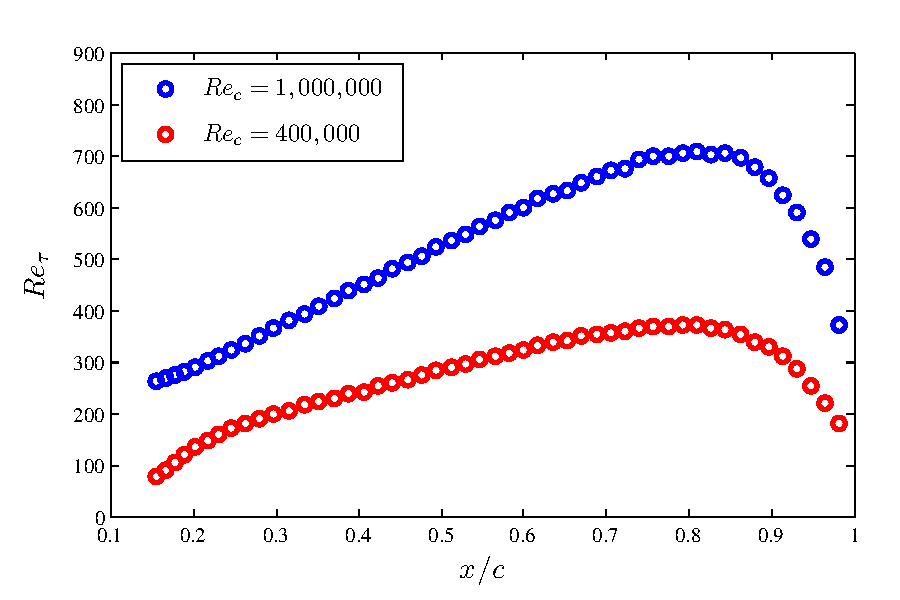
\includegraphics[width=0.49\textwidth]{paper4/imgs/Ret_vs_x}
	\caption{Streamwise evolution of (top left) the Clauser pressure-gradient parameter $\beta$, (top right) the Reynolds number based on momentum thickness $Re_{\theta}$ and (bottom) the friction Reynolds number $Re_{\tau}$, for the two wing cases under study.}
	\label{fig:overview_beta_Reth_Ret}
\end{figure}

%===============================================================================
\chapter{Conclusions and outlook}
%===============================================================================

The current thesis work concerns three different fields of research.

In the first part of the thesis, the ``evolve and filter'' technique for the stabilization of spectral-element methods is analyzed and it is found the filter operation causes an undesirable loss of divergence-free quality of the solution. This loss of divergence is shown to be particularly large for the test case of a double shear layer. An alternate formulation of the stabilization called the relaxation-term (RT) stabilization is shown to overcome the drawbacks of the explicit filtering technique, while maintaining the simplicity of the original explicit filter. This RT stabilization technique is very closely related to explicit filtering, with the two operations being equivalent to the leading order in time. Stability limits of the RT stabilization are explored and is shown to be stable within the practical parameter range.

In the second part, an NLF airfoil undergoing small-amplitude pitch-oscillations is analyzed at two different Reynolds numbers. In both cases a large variation of transition, and thus boundary layer characteristics is observed over the airfoil resulting in a non-linear response of the aerodynamic force coefficients. For $Re_{c}=750,000$ it shown that the temporal evolution of the transition point can be understood with a simple phase-lag concept, with the implication that boundary-layer evolution may be considered quasi-steady in time. Using this phase-lag concept a simple empirical model is developed which is able to explain a fairly wide range of experimental data.

On the other hand, for $Re_{c}=100,000$ a qualitatively different picture emerges for the unsteady boundary layer. The boundary-layer response displays a dynamically rich behavior with marked asymmetry of upstream and downstream transition movement. In this case, transition location is governed by the properties of the leading-edge laminar separation bubble (LSB) and it is conjectured that the absolute instability of the LSB may be responsible for abrupt changes in boundary layer characteristics.

Finally, in the third part of the study, flow over a stationary NACA 4412 airfoil is studied at two different Reynolds numbers with the aim of better understanding the boundary-layer evolution in non-equilibrium pressure gradient boundary layers. Two flow cases at a chord-based Reynolds number of $Re_{c}=400,000$ and $Re_{c}=1,000,000$ are compared at different streamwise locations. It is found that the effect of the streamwise pressure gradients is higher at low Reynolds numbers, leading to greater energy in the larger structures present in the outer part of the turbulent boundary layer.

The current work has laid the foundation for several interesting questions that may be the focus of future work. Can the simple empirical aerodynamic model be extended for a wider range of unsteady motions? Can the phase-lag be predicted a-priori as in the case of the classical model by \cite{theodorsen35}? When does the quasi-steady assumption break down and the boundary layer becomes truly unsteady? For $Re_{c}=100,000$, can the asymmetry of the (upstream and downstream) velocities of transition point be linked with the stability properties of the LSB? What is the influence of free-stream turbulence on unsteady LSB? In stationary airfoils, how does the velocity spectrum change with Reynolds number in non-equilibrium flows? What are the characteristics of boundary layer streaks in non-equilibrium flows? Some of these questions will be the focus of further research.


%===============================================================================
% Acknowledgments
%===============================================================================
%


\begin{acknowledgements}
	My foremost gratitude goes to my supervisor Dan Henningson for giving me the opportunity to join his research group. His knowledge and guidance have helped me immensely as a student. His encouragement, for which there is no substitute, have always provided the inspiration I needed to constantly push myself further in my work. Next I would like to thank my co-advisors Philipp Schlatter and Ardeshir Hanifi. Philipp for his patience during all my ignorant and sometimes foolish questions on numerics, conferences, papers and others that I probably can't recall. Ardeshir for the laughter, the sandwiches, the beers and most importantly, always being available on short notice when I needed help. I would also like to thank the members of the NFFP project, Roger Larsson, Dr. David Eller and Dr. Mikaela Lokatt for all the interesting discussions on aerodynamics. 
	
	I am grateful to Adam Peplinski for all the help he provided with Nek5000, MPI and coding in general. I can not imagine figuring out the workings of Nek5000 without his support. Armin and Ricardo have helped me more than others during my crucial time as a new Phd student. The help is greatly appreciated.
	
	Special mentions go to Mattias for all the coffee breaks, introducing me to Swedish food, the spontaneous discussions and being the bouncing board for all my (mostly wrong) ideas. Your company shall be missed once you leave the department. Jacopo and Giandomenico for all the great company, joining for the spontaneous plans and granting me the honorary Italian citizenship. I'll learn Italian very soon I promise! Marco for the constant dinner company. Freddy for the weekend food+beer+movie routine. Elektra for being one of the greatest friends of all time. Politics, late-night and of course Trump shall keep us entertained for times to come. But mostly, thanks for correcting my manuscripts and the support during this licentiate period. A mention must also go to my unrequited love, Walter Fornari. Where will I find another like you?
	
	A hearty thanks goes out to all my friends here at the department who make this a wonderful place. Eric, Clio, Nicolas, Sudhakar, Ugis, Evelyn, Anthony, Mehdi, Ali, Guillaume, Luca, Luca, Pierluigi, enrico, Francesco, Kristina, Ekatrina, J.C., Matthias, Priti, Ninge, Sagar, Krishne, Dhiya, and everyone else. All of you, with your quirks, jokes, stories and gossip (looking at you Pierluigi) add a little bit of color to life everyday.
	
	Perhaps most importantly, my deepest gratitude goes towards my family for their patience, unconditional love and support during my ever wandering path through life.
	
	Lastly, financial support for this work was provided by Vinnova through the NFFP project UMTAPS, with grant number 2014-00933, the Knut and Alice Wallenberg Foundation, and the European Research Council under grant agreement 694452-TRANSEP-ERC-2015-AdG.\ The computations were performed on resources provided by the Swedish National Infrastructure for Computing (SNIC) at the PDC Center for High Performance Computing at the Royal Institute of Technology (KTH). Simulation have also been performed at the Barcelona Supercomputing Center, Barcelona, with computer time provided by the $12^{th}$ PRACE Project Access Call (number 2015133182) and at the High Performance Computing Center, Stuttgart (HLRS) with the computer time provided by the $15^{th}$ PRACE Project Access Call (number 2016163965). 

\end{acknowledgements}



%===============================================================================
% References
%===============================================================================
%
\bibliographystyle{jfm}
\bibliography{licentiate}
%
\IfFileExists{overview.bbl}{\graphicspath{{imgs/}}
%\setlength{\captionmargin}{50pt}

%===============================================================================
\chapter{Introduction}
%===============================================================================
\section{A short history}

The first sustained flight by the Wright brothers in 1903 marked a historic day in human achievement and ingenuity. Momentous as the achievement was, the Wright brothers did not truly invent the modern airplane. Their achievements were the fruition of nearly a century of aeronautical research, starting perhaps with Sir George Cayley, who is considered the ``father of aerial navigation'' \citep{gibbs-smith62}. The principal components of the modern aircraft were laid down by George Cayley as early as 1799. Prior to Cayley, the ideas for mechanical flight tended towards flapping wings, where the flapping motion produced both propulsion and lift. George Cayley was the first to break the unsuccessful chain of thought and separated the two aspects of flight into distinct systems. His triple paper ``On Aerial Navigation'' published in Nicholason's \textit{Journal of Natural Philosophy, Chemistry and the Arts} on November 1809, February and March 1810 \citep{cayley1809} mark some of the most important works in aeronautical history. In the works, Cayley states for the first time, the principle of lift generation \textit{i.e.} the formation of a low pressure region on the upper surface of the wing. His paper elaborates on the separation of lift from propulsion and also goes on to talk about flight control and airplane stability. Later in his life, he proposed the concept of multiplanes (multiple wings mounted on top of each other) and built the first glider triplane named the ``boy carrier'' in 1849.

Several investigators followed the quest of ``aerial navigation''. Otto Lilienthal was the first to design and successfully fly controlled gliders in 1891, going on to make over $2500$ successful glider flights. Octave Chanute brought aeronautics research to America and designed a biplane glider which directly inspired the designs of the Wright Brothers. Samuel Pierpont Langley was a contemporary of the Wright brothers who built and tested several powered model airplanes. His success in achieving powered flight directly influenced and encouraged the Wright brothers. The final historic achievement of successful powered flight was achieved by the Wright brothers. On December $17^{th}$ 1903, a gasoline powered biplane by the name Wright Flyer I (figure~\ref{fig:wright_flight}) took flight in (modern day) Kill Devil Hills, North Carolina, ushering forth the era of practical human flight.
\begin{figure}[h]
	\centering
	\includegraphics[width=0.90\textwidth]{wright_brothers_first_flight}
	\vspace{10pt}	
	\caption{First flight of the Wright Flyer I, December 17, 1903, Orville piloting, Wilbur running at wingtip. Image from \cite{wikipedia_wright}.}
	\label{fig:wright_flight}
\end{figure}

\section{Modern aircraft design}
Since that fateful day, modern airplanes have been used in a variety of different conditions, varying from commercial passenger planes, to supersonic military aircrafts \citep{blackbird}, 
to endurance flights around the world lasting 9 days \citep{rutan_voyager}. The myriad uses have resulted in various challenges that need to be overcome by the aircraft designers. One significant challenge has been due to the dynamic interaction of air flow with the airplane structures, now studied under the field of aeroelasticity. These problems came to the fore as the design speed of aircrafts increased over the years and designers came to favor monoplanes over the biplane design. An early example was that of the Fokker D-8 German aircraft during World War I which suffered wing failure under steep dives, which was the first documented case of static aeroelastic effects.

Today the designers of commercial aircrafts face another challenge brought about by global climate change and rising oil prices. With the realization of the contribution of the aviation industry towards global climate change \citep{green08}, aircraft designers now face a need to significantly improve the fuel efficiency of commercial aircrafts in a bid to reduce the carbon footprint of the industry. In an effort to quantify the opportunities of achieving such an improvement, \cite{schrauf05} showed a break-down of the drag experienced by a typical transport aircraft highlighting that frictional drag accounted for more than half the drag experienced by the aircraft. Clearly a favorable modulation of the boundary layer over the wing could help achieve large improvements in fuel efficiency. The modulation could come in the form of effective flow control strategies, or with wing design strategies such as the use of natural laminar flow (NLF) airfoils. Both \cite{schrauf05} and \cite{green08} push forward the idea that NLF airfoils and laminar flow control strategies are the low-hanging fruits in the goal of higher fuel efficiency and a concerted effort into addressing the engineering challenges for practical implementation must be made. Some of these challenges may require revisiting the aeroelasticity problems from the perspective of laminar wings. However laminar flow at high Reynolds numbers is susceptible to destabilization and may not always be possible. Thus turbulent drag reduction strategies need to be used effectively where needed \citep{bushnell03}. Whatever the form of drag reduction technique that may finally be implemented on a particular aircraft, the understanding of developing boundary layers over wings (including the influence of control strategies) occupies a central position in aerodynamic research if the goal of higher fuel efficiency is to be realized. With this goal in mind, the current thesis work aims to further the understanding of developing boundary layers over airplane wings, focusing on two particular aspects.
\begin{itemize}
	\item Understanding the structure of the turbulent boundary layer developing over a wing section.	
	\item Understanding the evolution of the developing boundary layer over a natural laminar flow airfoil in unsteady flight conditions. 
\end{itemize}

%Solutions to these emerging aeroelastic problems needed an understanding of the unsteady phenomenon occurring in practical flight conditions. Such understanding came via the works of \cite{glauert30,karman38,theodorsen35} \textit{etc}, and by the 1940s, design engineers had the tools to account for unsteady aeroelastic effects in their wing designs.

%The achievements of these early aerdynamicists is quite impressive in particular considering that the boundary layer concept was in its nascent stages when the first practical airplanes were being designed. Indeed Prandtl's revolutionary concept of a boundary layer was first presented in 1904, almost a full year after the first flight of the Wright brothers.  

%-------------------------------------------------------------------------------
\section{Boundary layers over a stationary wing}

The understanding of the structure and scaling of wall-bounded turbulent flows has been in study for several decades and a complete understanding still remains far from complete. These flows have been studied with different canonical geometries such as channels \citep{kim87,moser99,lee15}, pipes \citep{elkhoury13,jimenez08,chin15} and flat plates \cite{spalart88,schlatter10,eitel14}. For the case of spatially evolving boundary layers over a flat plate, the simplest canonical case involves boundary-layer evolution subjected to a zero pressure gradient (ZPG). These flows may be uniquely characterized by a single parameter, \textit{i.e.} the Reynolds number Re, which is the ratio of the inertial and viscous scales of the flow. However practical flow cases are often influenced by pressure gradients. Such flow cases can no longer be uniquely defined using a single parameter. \cite{clauser54} with intuitive reasoning proposed a concept of an equilibrium boundary layer which may be uniquely defined by two parameters. He argued that, if the ratio of the average pressure gradient force across the boundary layer and the viscous shear force at the wall remains constant, the boundary layer would experience a similar flow history throughout its evolution. Thus the equilibrium pressure gradient boundary layers are uniquely defined by two parameters, namely the Reynolds number (Re) and the pressure gradient parameter $\beta$, defined as
\begin{eqnarray}
	\beta = \delta^{*}(dp/dx)/\tau_{w},
\end{eqnarray}
where $\delta^{*}$ is the displacement thickness, $dp/dx$ is the pressure gradient and $\tau_{w}$ is the wall-shear stress. The parameter is commonly referred to as the Clauser parameter. A flow case with a spatially constant Clauser parameter is categorized as an equilibrium boundary layer and a ZPG boundary layer is a special case of an equilibrium boundary layer with $\beta=0$. Several works have focused on pressure gradient boundary layers ranging from theoretical studies by \cite{townsend56,townsend56b,mellor66}, experimental works of \cite{skare94,harun13} and numerical simulations by \cite{spalart93,skote98}. The developing boundary layer over an airfoil however further increases in complexity since these boundary layers fall under the category of non-equilibrium boundary layers where the Clauser parameter is spatially varying. In such cases the flow history also plays a role in determining the local boundary layer properties \citep{clauser54,bobke17}. Analysis of such flow cases becomes significantly more difficult since the local boundary layer parameters do not uniquely define the state of the boundary layer. Nonetheless the study of such boundary layers is important since generic boundary layers found in nature would belong to this category, including the boundary layers over wings. The boundary layer developing over the NACA 4412 airfoil has the property that the spatially varying Clauser parameter is insensitive to Reynolds number. The presents us with the opportunity to study the Reynolds number effects of a non-equilibrium boundary layer with a constant pressure gradient history. That is indeed the methodology followed in this work. The developing boundary layer over a NACA 4412 wing section is analyzed at two different Reynolds numbers in order to understand Reynolds number effects in non-equilibrium boundary layers.

\section{Unsteady boundary layers}
%
Unsteady aeroydnamic studies started with the emergence of aeroelastic phenomenon in the early part of the $20^{th}$ century. With the gradual shift to monoplane designs, the inherent high torsional stiffness of biplanes was lost and aerodynamic instabilities, such as the one experienced by the Fokker D-8 became important. Pioneering works of \cite{glauert30,karman38,theodorsen35} \textit{etc}, provided the insight and modeling of such unsteady aerodynamic behavior and by the 1940s the foundations of unsteady aerodynamics for incompressible attached flows had been laid down. The mathematical framework these unsteady aerodynamic theories relied on simple inviscid and quasi-steady assumptions, which proved to be highly attractive to the wing designers \citep{leishman00}. Experimental corroboration by \cite{halfman52} and \cite{rainey57} further added support to the validity of the simple assumptions. Over the next few decades, investigations of unsteady aerodynamics shifted focus to the understanding of the dynamic stall phenomenon, with works of \cite{mccroskey76,mccroskey81,mccroskey82experimental,mccroskey82,carr1977,crisler94}. A large body of work on unsteady separated flows was presented by \cite{ericsson86,ericsson87b,ericsson_stall88a,ericsson_stall88b}. The studies continue to this day with the works of \cite{visbal11,visbal14,visbal17,dunne2015} and several other authors, a recent review can be found in \cite{coorke15}. 
\begin{figure}[h]
	\centering
	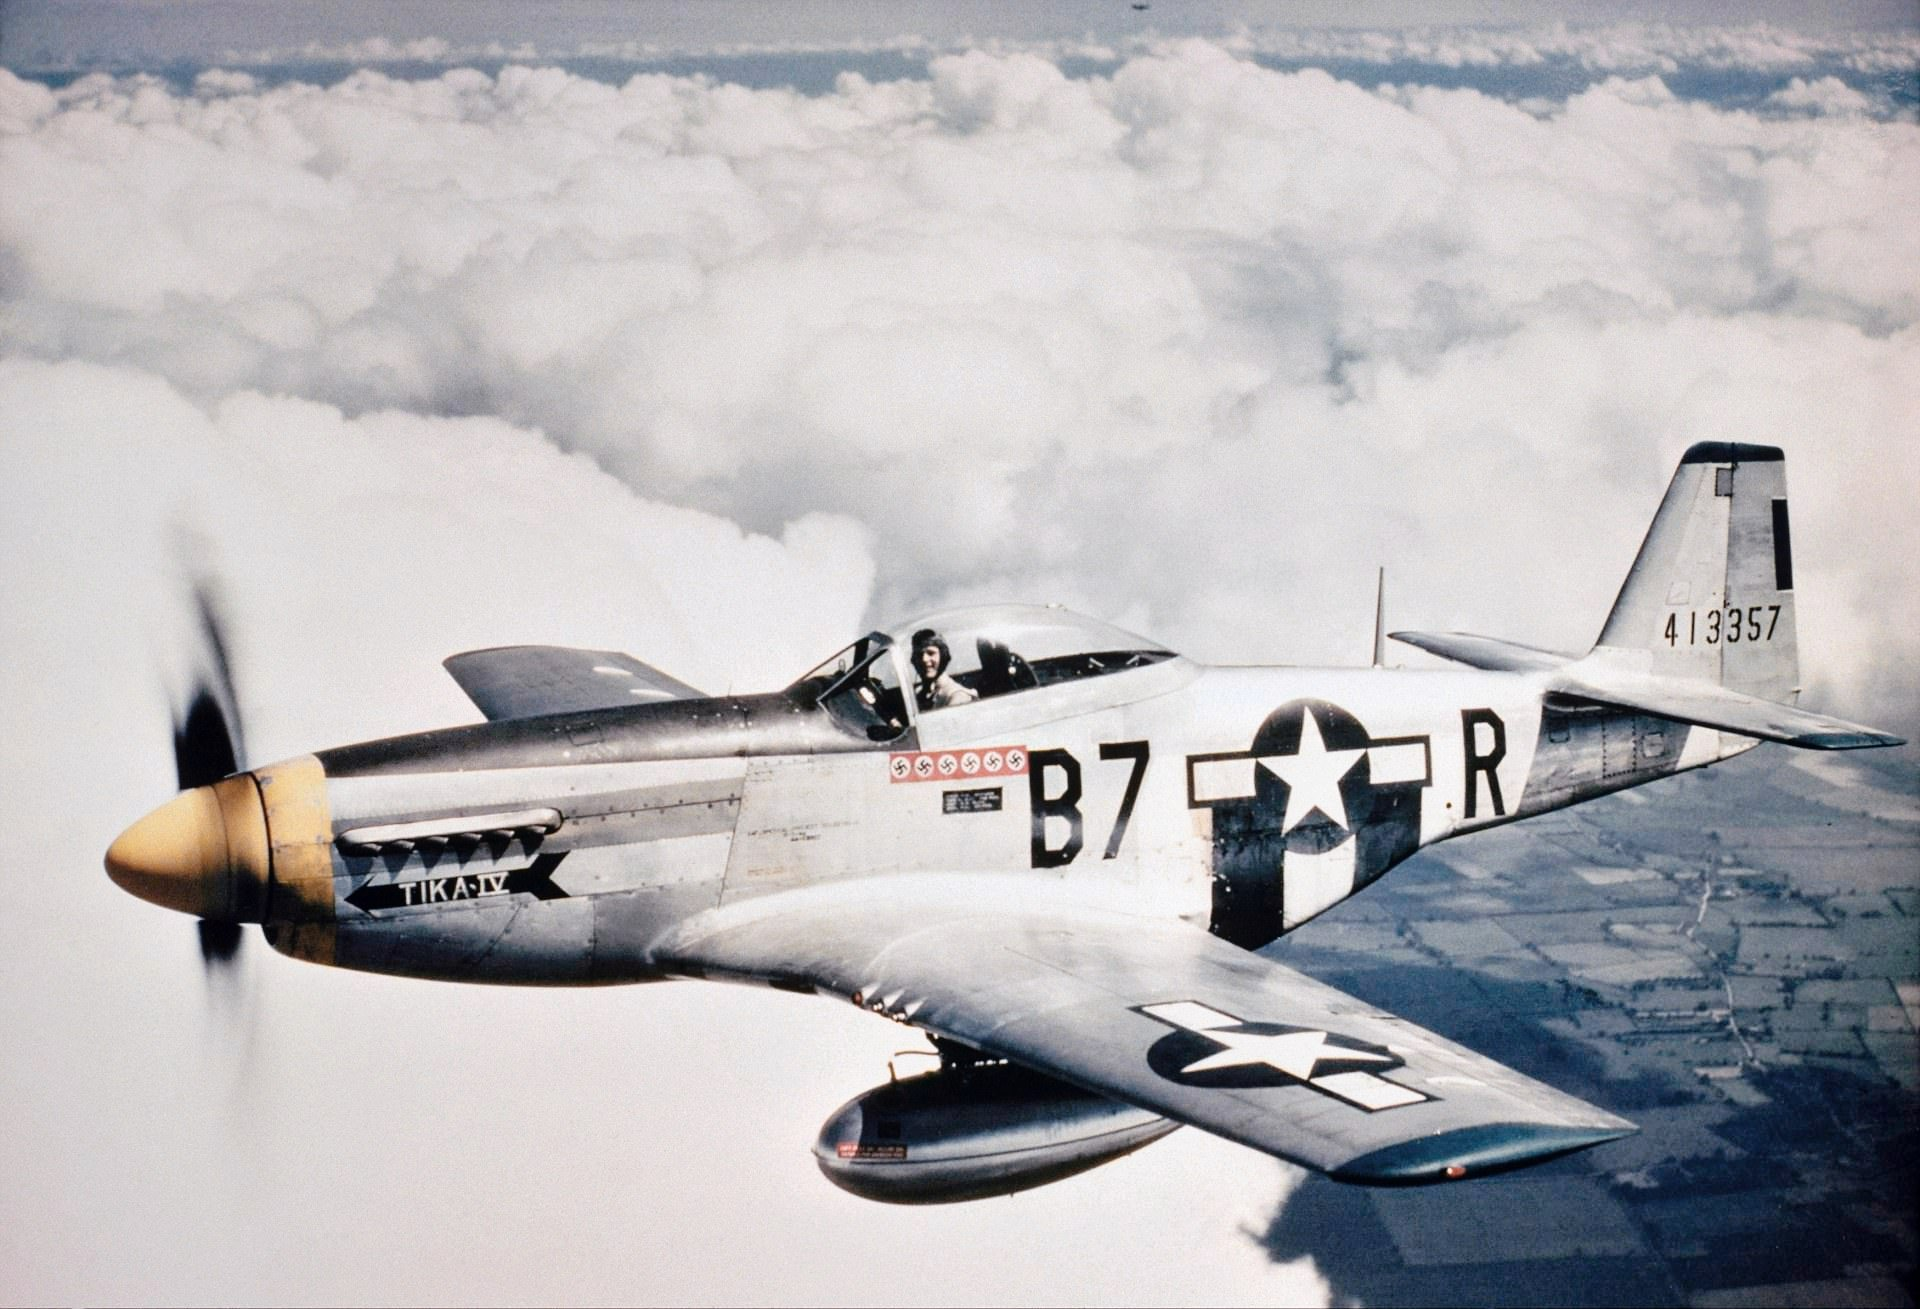
\includegraphics[width=0.90\textwidth]{P-51-mustang}
	\vspace{10pt}
	\caption{North American P-51 Mustang. Image from \cite{wikipedia_mustang}.}
	\label{fig:mustang}
\end{figure}

However it appears that the aeroelasticity problem was not considered from the perspective of natural laminar flow airfoils. This is a surprising fact considering the P-51 Mustang (figure~\ref{fig:mustang}), a fighter aircraft in the Royal Air Force designed in 1940, incorporated a wing with a natural laminar flow airfoil section \citep{green08}. The first aeroelastic study on laminar wings was performed as late as 2011 by \cite{mai11}. This, along with a subsequent investigation by \cite{hebler13}, brought to light a peculiar characteristic of unsteady laminar wings, \textit{i.e.} the presence of non-linearities in the unsteady aerodynamic forces. The classical unsteady aerodynamic theories did not predict non-linear unsteady responses and thus fail to account for such behavior. Inspired by this, \cite{lokattthesis} performed experiments on unsteady NLF airfoils and also found strong non-linearities in the aerodynamic forces. Consistent in the explanation for the non-linearities in all these studies was the role of transition over the wing surface. When transition on the airfoil suction-side was fixed (with a trip) near the leading edge, the non-linearities seemed to disappear. These results indicated a need for a more in-depth study of the evolving boundary layer in such unsteady laminar airfoils. Classical theories negate the role of the boundary layer by invoking the inviscid assumption and it is apparent that such an assumption is no longer be justified for laminar wings. Characteristics of the unsteady boundary layer are the subject of investigation in the present work.

\thesisstructure The thesis is structured as follows:
\begin{itemize}
	\item An overview of the numerical method used for the simulations is given in Chapter 2.
	\item Chapter 3 gives an overview of the numerical simulations performed in the study.
	\item The main conclusions of the current work are given in Chapter 4 along with an outlook for future work.
	\item The next part of the thesis includes the individual papers and internal reports. 
\end{itemize}

%===============================================================================
\chapter{Numerical Method}
%===============================================================================

\section{Numerical Discretization}

The numerical code used for the simulations is Nek5000, which is an open source research code developed by \cite{nek5000} at Argonne National Laboratory. The code solves the incompressible Navier--Stokes equations (\ref{eqn:navier_stokes}) in non-dimensional form:
\begin{subequations}
	\label{eqn:navier_stokes}	
	\begin{eqnarray}
	\frac{\partial u_{i}}{\partial t} + u_{j}\frac{\partial u_{i}}{\partial x_{j}} =  - \frac{1}{\rho}\frac{\partial p}{\partial x_{i}} + \frac{1}{Re}\bigg(\frac{\partial^{2} u_{i}}{\partial x_{j}\partial x_{j}}  \bigg) +f_{i} \\
	\frac{\partial u_{i}}{\partial x_{i}} = 0
	\end{eqnarray}
\end{subequations}
where $x_{i}$ is the coordinate direction, $u_{i}$ is the velocity component, $p$ is the pressure and $Re$ is the defined Reynolds number. The discretization of the Navier--Stokes equations is based on a spectral-element method, first proposed by \cite{patera84}. The method allows the mapping of elements to complex geometries along with a high-order spatial discretization within the elements, thus combining the generality of finite-element methods with the accuracy of spectral methods \citep{patera84}.
The spatial discretization in each element is performed following the $P_{N}$-$P_{N-2}$ \citep{maday89} formulation with velocity represented by high-order Lagrange interpolants through the Gauss--Lobatto--Legendre (GLL) quadrature points, while the pressure is represented on the staggered Gauss-Legendre (GL) quadrature points. The nonlinear terms are treated explicitly by third-order extrapolation (EXT3), while the viscous terms are treated implicitly by a third-order backward differentiation scheme (BDF3). Over-integration is used for the removal of aliasing errors. Nek5000 is written in Fortran 77 and C with efficient scaling for up to 1 million MPI ranks \citep{fischer15}.

%%%%%%%%%%%%%%%%%%%%%%%%%%%%%%%%%%%%%%%%%%%%%%%%%%%%%%%%%%%%%%%%%%%%%%
\section{Relaxation-term large-eddy simulation (RT-LES)}

Owing to the high Reynolds numbers and large time-scales of integration for some of the flow cases, a direct numerical simulation (DNS), which requires a resolution of all the spatial scales of the flow, leads to prohibitively high computational costs. In recent years a technique of wall-resolved large-eddy simulations has emerged as a computationally cheaper alternative to DNS, while also exhibiting the high-fidelity characteristics of DNS.
The technique has been utilized in the studies of spatially developing boundary layers \citep{eitel14}, pipe flows \citep{chin15} and flow over wings \citep{uzun10,lombard15}. The success of the approach has motivated its use in the present work. The wall-resolved LES method used is based on the RT3D variant of the ADM-RT approach first used by \cite{schlatter04}. The method has been shown to be reliable in accurately predicting transition and also preserving the characteristic structures which are seen in the DNS of transitional flows by \cite{schlatter06}. This particular quality of the LES model is crucial since there is a large focus on the unsteady transition in the present work. The LES method supplements the governing equations with a dissipative term $-\chi\mathcal{H}(u)$. The equations of motion for the resolved velocity and pressure thus read as
\begin{subequations}
	\label{eqn:rt_les}	
	\begin{eqnarray}
	\frac{\partial u_{i}}{\partial t} + u_{j}\frac{\partial u_{i}}{\partial x_{j}} =  - \frac{1}{\rho}\frac{\partial p}{\partial x_{i}} + \frac{1}{Re}\bigg(\frac{\partial^{2} u_{i}}{\partial x_{j}\partial x_{j}}  \bigg) + f_{i} -\chi\mathcal{H}(u_{i}), \\
	\frac{\partial u_{i}}{\partial x_{i}} = 0,
	\end{eqnarray}
\end{subequations}	
where $\mathcal{H}$ is a defined high-pass spectral filter and $\chi$ is a model parameter which together with $\mathcal{H}$ determines the strength of the dissipative term. The high-pass filter function $\mathcal{H}$ is defined such that the resultant relaxation-term only has energy in the highest modes, defined by a cut-off mode-number $N_{c}$. Figure~\ref{fig:filter_shape} illustrates the shape of the filter function in spectral space.
\begin{figure}[h]
	\centering
	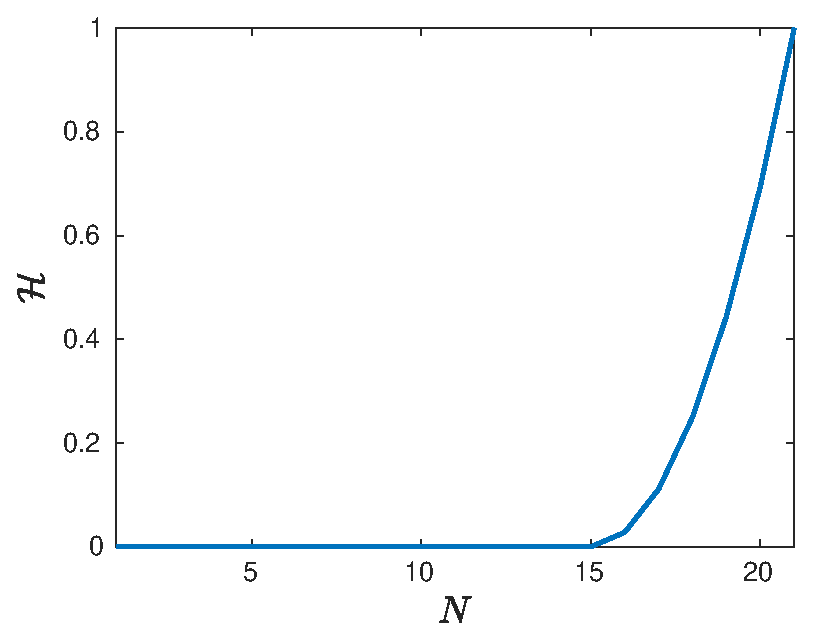
\includegraphics[width=0.60\textwidth]{filter_shape}
	\caption{Transfer function for the spectral coefficients for the filter $\mathcal{H}$ with number of modes $N=21$ and cut-off mode number $N_{c}=16$.}
	\label{fig:filter_shape}
\end{figure}

Several parameter optimization studies were performed to determine the optimum value of $\chi$ and filter shape $\mathcal{H}$ using turbulent channel flow simulations. The LES results were compared with the DNS database of \cite{moser99} and the optimum parameters were further validated for a flow around a wing section at $Re_{c}=400,000$. A good agreement was found between the LES and the DNS data of \cite{hosseini16}, and the optimized parameters were then used for all subsequent simulations.

\section{Arbitrary-Lagrangian-Eulerian (ALE)}

Typical solutions of unsteady fluid flows utilize the Eulerian framework where the coordinate system is fixed in space. A fixed coordinate system however becomes infeasible when the domain boundaries are in motion, as is the case of fluid-structure interaction problems, or when there is a free surface which may lead to a deforming interface. An appropriate method is needed to account or the motion of the boundaries and/or the interior grid points. One such method which substantially simplifies the difficulties arising out of moving boundaries is the Arbitrary-Lagrangian-Eulerian (ALE) method. The method was proposed in a finite-difference framework by \cite{hirt74} and later brought to the spectral-element framework by \cite{ho90,ho91}. The technique combines both the Lagrangian and Eulerian formulations such that, the Navier--Stokes may be solved with the grid points moving with the fluid elements \textit{i.e.} in a Lagrangian framework, or with fixed grid points (Eulerian), or with grid points moving in an arbitrary prescribed manner. The heart of the technique lies in the formulation of the total time rate of change of a quantity in the ALE frame, defined analogously to the material derivative. Thus for a quantity $\mathbf{F(x_{i},t)}$, the change due to small increments $dx_{i}$ and $dt$ may be expressed as \citep{kundu02}
\begin{align}
	dF = \frac{\partial F}{\partial t}dt + \frac{\partial F}{\partial x_{i}}dx_{i}.
	\label{eqn:material_deriv_df}
\end{align}
One may choose to follow any arbitrary path along which this quantity is evaluated, in which case the quantities $dx_{i}$ and $dt$ are related by the velocity of the (grid) point along this arbitrary path $w_{i} = dx_{i}/dt$. The relation results in the expression referred to as the ALE derivative \citep{deville02}, here denoted as $\delta F/\delta t$ to differentiate it from the very similar expression for the material derivative (which is evaluated along the fluid particle trajectory)
\begin{align}
\frac{\delta F}{\delta t} = \frac{\partial F}{\partial t} + w_{i}\frac{\partial F}{\partial x_{i}}.
\label{eqn:ale_derivative}
\end{align}
When $w_{i}$ is equal to the fluid velocity $u_{i}$, we recover the familiar Lagrangian expression for the material derivative $DF/Dt$. On the other hand, when $w_{i}=0$, we get the local (Eulerian) rate of change of the quantity $F$. The material derivative and the ALE derivative share a simple relationship defined using a relative velocity of the fluid particle with respect to the grid motion $c_{i} = u_{i} - w_{i}$, which may be used in the definition of material derivative to obtain
%\begin{subequations}
	\begin{align}
%	\frac{DF}{Dt} = \frac{\partial F}{\partial t} + u_{i}\frac{\partial F}{\partial x_{i}} \nonumber\\
%	\frac{DF}{Dt} = \bigg(\frac{\partial F}{\partial t} + w_{i}\frac{\partial F}{\partial x_{i}}\bigg) + c_{i}\frac{\partial F}{\partial x_{i}} \nonumber \\	
	\frac{DF}{Dt} = \frac{\delta F}{\delta t} + c_{i}\frac{\partial F}{\partial x_{i}}.
	\label{eqn:ale_material_derivative}
	\end{align}
%\end{subequations}
Thus the Navier--Stokes in the ALE formulation may be expressed as 
\begin{subequations}
	\label{eqn:ale_navier_stokes}	
	\begin{align}
	\frac{\delta u_{i}}{\delta t} + (u_{j} - w_{j})\frac{\partial u_{i}}{\partial x_{j}} =  - \frac{1}{\rho}\frac{\partial p}{\partial x_{i}} + \frac{1}{Re}\bigg(\frac{\partial^{2} u_{i}}{\partial x_{j}\partial x_{j}}  \bigg) +f_{i}, \\
	\frac{\partial u_{i}}{\partial x_{i}} = 0,
	\end{align}
\end{subequations}
where $w_{j}$ is the velocity of the grid points. The solution of the Navier--Stokes is then a simple matter of evaluating a suitable grid velocity. 

In many cases, such as the flow over an oscillating airfoil, the velocity of the grid points at the boundary (airfoil surface) may be explicitly known. \cite{ho90,ho91} propose to extend this velocity to the interior points of the domain by solving an elliptic problem for the mesh velocity. In the present work we take a simpler approach to prescribing the mesh velocities in the interior domain. Recognizing the simple trigonometric form of a harmonic pitching motion, all mesh points may simply be prescribed a solid body rotation with the instantaneous angular velocity of the airfoil. However a pure solid-body rotation would also displace the domain boundaries. Therefore a damping function is used to smoothly reduce the rotational velocity away from the airfoil boundary such that the mesh motion is zero at the far-field, inlet and outflow boundaries. Thus for an airfoil with an instantaneous rotation rate of $\Omega_{z}(t)$, the mesh velocity is prescribed as:
\begin{align}
	w_{i}(x,y,z,t) = \underbrace{(\Omega_{z}(t) \times \vec{R})}_{\text{Solid body rotation}} \overbrace{f(|\ \vec{r}\ |)}^{Damping}
	\label{eqn:mesh_velocity}
\end{align}
where $\vec{r}$ is the normal distance of a grid point from the airfoil surface, $\vec{R}$ is the distance from the rotational axis and $f(r)$ is a damping function which can be prescribed in many different ways, depending on one's preferences. The damping function needs to have two essential properties, \textit{i.e.} it must be equal to 1 when $|\vec{r}|=0$, which implies the mesh points at the airfoil boundary move with the surface (solid body rotation at the airfoil surface), and it must smoothly decay to zero close to the far-field boundaries, which allows the external boundaries of the computational domain to remain fixed in physical space. Figure~\ref{fig:mesh_rotation_damping} shows the damping function used in the present work as a function of the normal distance from the airfoil surface.
\begin{figure}[h]
	\centering
	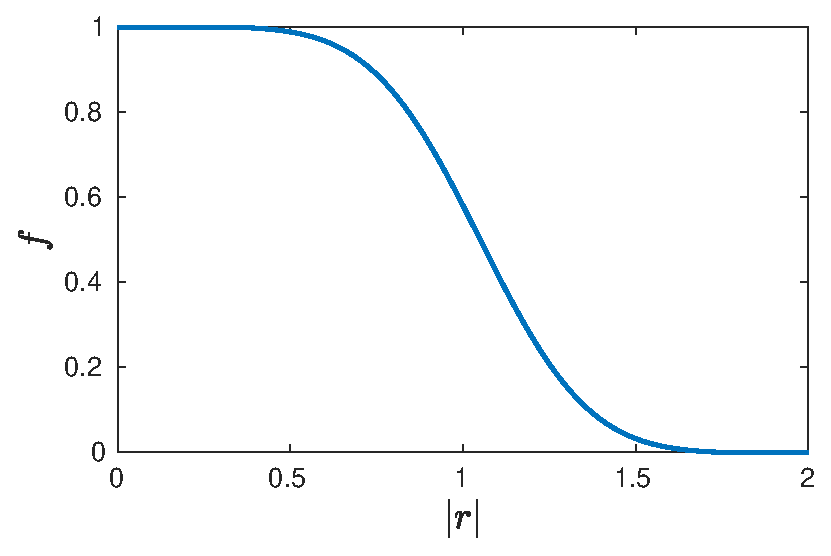
\includegraphics[width=0.55\textwidth]{damping_func}
	\vspace{5pt}
	\caption{Damping function $f(r)$ for the mesh velocities.}
	\label{fig:mesh_rotation_damping}
\end{figure}
The damping function moves the grid points close to the airfoil surface with the same rotational velocity of the airfoil and spreads out the mesh deformation into the interior of the domain. This damping function is calculated once at the beginning of the simulation. Hence all quantities $\Omega_{z}(t),\ \vec{r},\ f(r)$ which are needed for prescribing the mesh velocity are explicitly known at each time-step without the need for solving an elliptic equation as in \cite{ho90,ho91}. 

\section{Free-stream turbulence}

Isotropic, homogeneous free-stream turbulence is prescribed at the inlet and far-field boundaries to add small disturbances to the flow-field, which simulate the disturbances found in a wind-tunnel or in free-flight conditions. The free-stream turbulence is prescribed as a superposition of Fourier modes with a random phase shift. The maximum and minimum amplitudes of the wavenumber vector are prescribed quantities and are limited by the resolution of the spatial discretization and size of the domain respectively. The wavenumber space between the minimum and the maximum is divided into 20 concentric shells with each shell representing the amplitude of the three-dimensional wavenumber vectors lying on the shell. 20 points are randomly chosen on each shell with the location of each point representing the three-dimensional components of the wavenumber vector. Thus the free-stream turbulence is represented by a total of 400 fourier modes. Care is taken to avoid very small wavenumber components which result in wavelengths in physical space that are larger than the computational domain. The streamwise length scales are transformed to a temporal frequency by invoking Taylor's frozen turbulence hypothesis and using the local mean streamwise velocity at the inlet for the space-time conversion. The amplitude of the free-stream modes on each spherical shell is scaled using the von K\'arm\'an spectrum. Figure~\ref{fig:fst_duct} shows an instantaneous visualization of the streamwise velocities in a doubly-periodic duct flow case with high ($5\%$) free-stream turbulence intensity prescribed at the the inlet. Figure~\ref{fig:ti_decay} shows the spatial decay of turbulence intensity. After a small initial distance of adjustment from the inlet, the turbulence intensity decays as a power law. A very similar method for generating free-stream turbulence for simulations of flat-plate boundary layers is used by \cite{schlatterdiploma,brandt04,schlatter08} and more recently for wind turbine simulations by \cite{kleusberglicenciate}.

\begin{figure}[h]
	\centering
	\begin{subfigure}[t]{0.49\textwidth}
		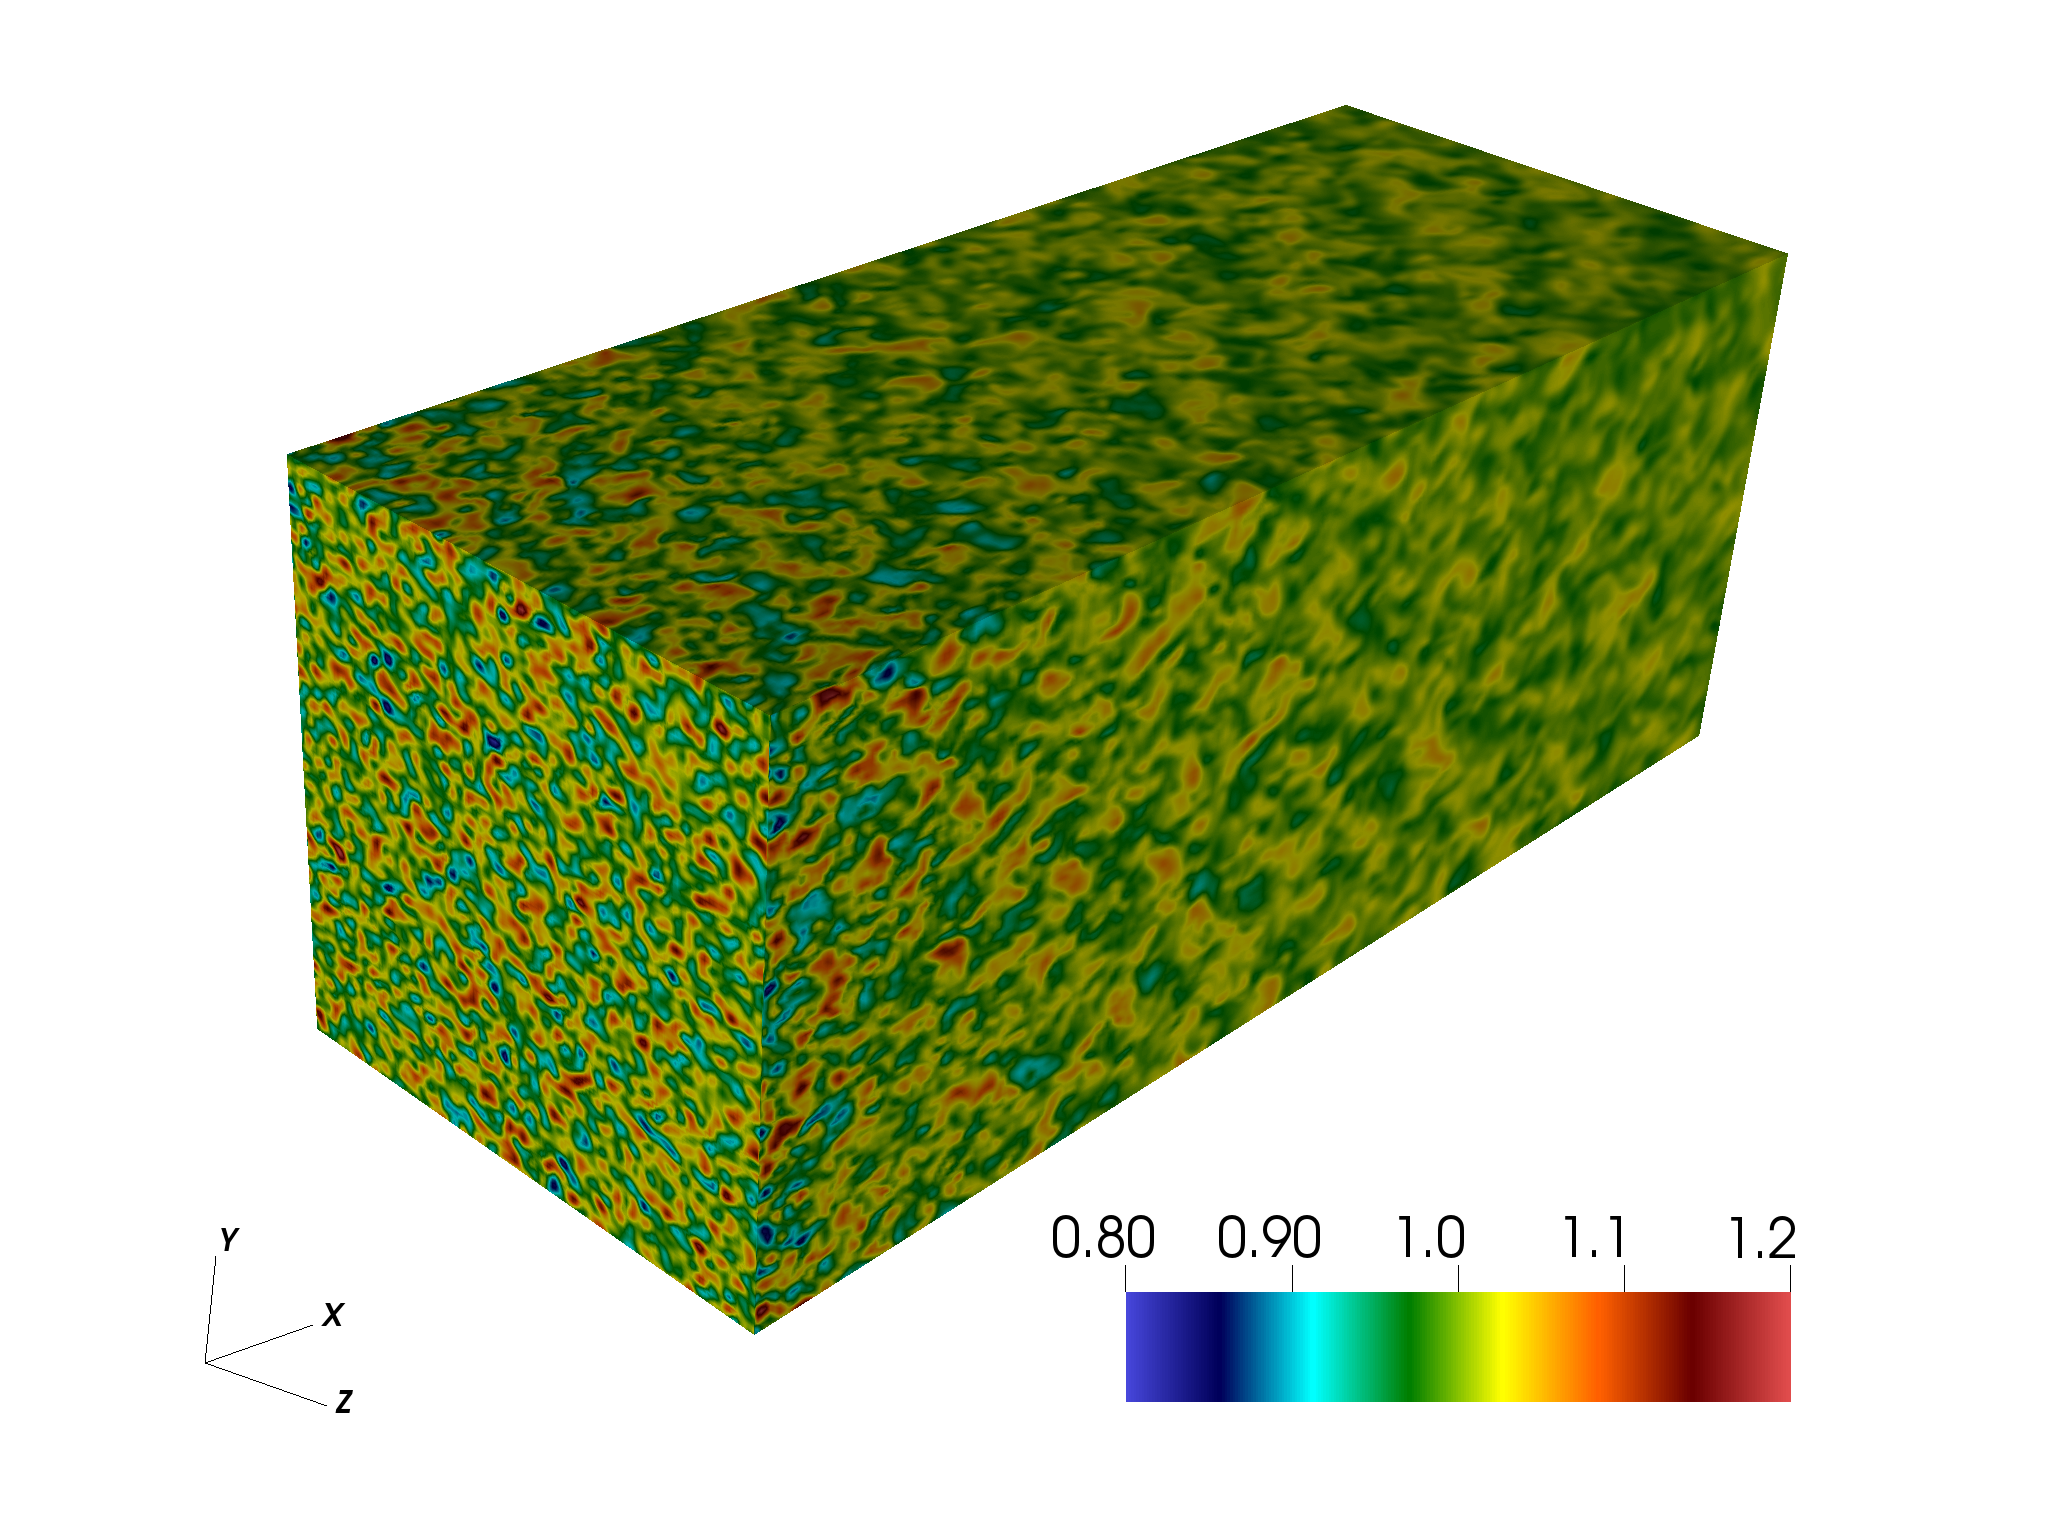
\includegraphics[width=1\textwidth]{fst_duct_vx0000.png}
		\caption{Visualization of free-stream turbulence prescribed at the inlet for a doubly periodic duct flow. Colors represent the instantaneous streamwise velocity.}
		\label{fig:fst_duct}
	\end{subfigure}
	\begin{subfigure}[t]{0.49\textwidth}
		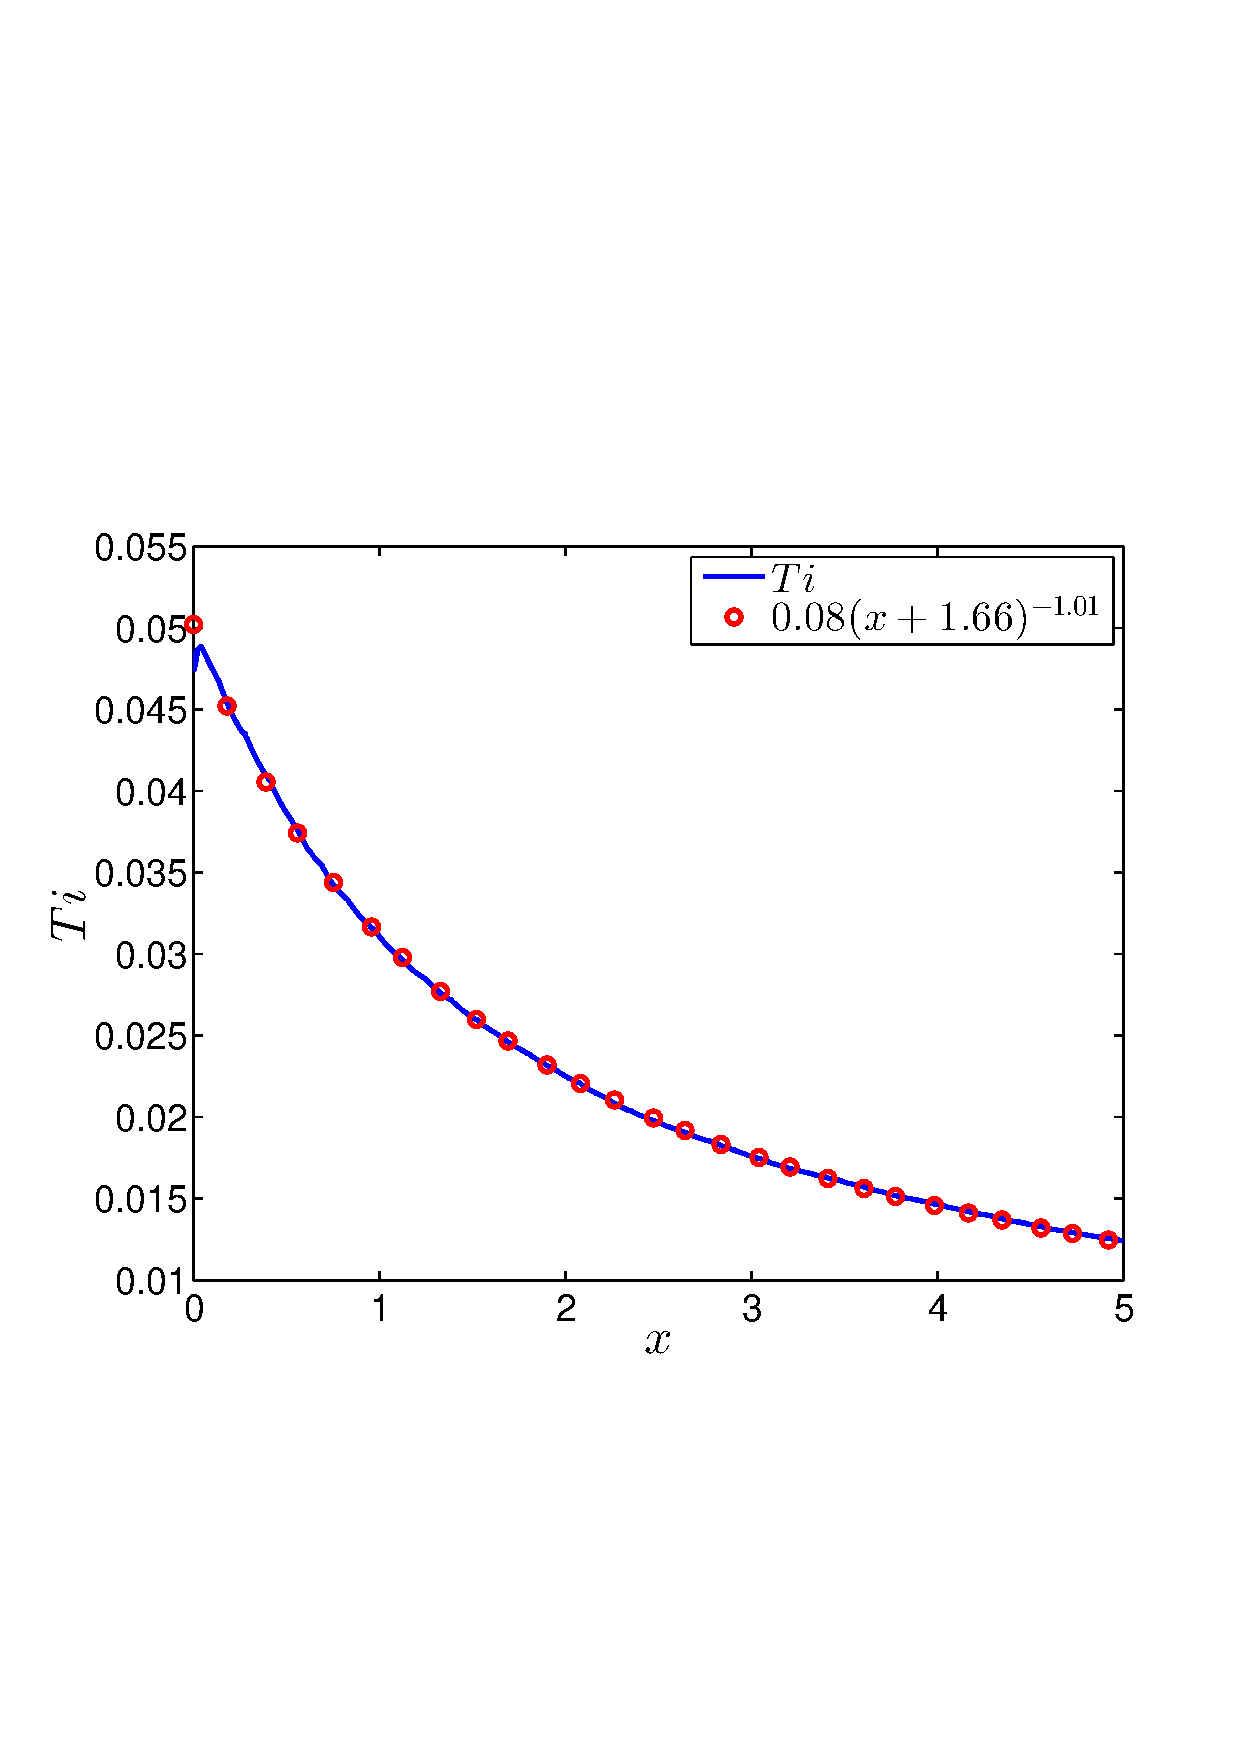
\includegraphics[width=1\textwidth]{ti_decay}
		\caption{Decay of turbulence intensity with streamwise distance, along with the least-squares fit of a power law.}
		\label{fig:ti_decay}
	\end{subfigure}
\end{figure}

%===============================================================================
\chapter{Overview of numerical simulations}
%===============================================================================

\section{Flow around unsteady wings}

The unsteady experiments of \cite{mai11,hebler13} and \cite{lokattthesis} have shown that aerodynamic non-linearities are related to the movement of transition over the suction side of the airfoil. Thus unsteady boundary layer dynamics play an important role in aerodynamic response of NLF airfoils. The present work investigates the unsteady boundary layers with a particular focus on unsteady transition with the aim to shed light on the phenomenon of non-linear unsteady aerodynamic response. The airfoil used in the investigation is the ED36F128 (with a $13.8^{\circ}$ flap deflection), designed at the Aeronautical and Vehicle Engineering department at KTH. It is a natural laminar flow airfoil, which has been used in several steady and unsteady experiments \citep{lokatt17,lokattthesis}. The unsteady experiments have shown the non-linearities that appear to be typical of laminar airfoils \citep{lokattthesis}. The results of the steady and unsteady experiments using this airfoil have been made available to us by Dr. Eller and Dr. Lokatt. Non-linearities in the unsteady aerodynamic forces are observed for only a certain range of angle of attack $\alpha$. Therefore a careful assessment of the data was needed in order to select the right parameter range where the relevant flow physics could be observed in the numerical simulations. The data in the experimental campaign was gathered primarily through pressure taps located around airfoil for the calculation of unsteady aerodynamic forces. Thus measurements of the unsteady boundary layer characteristics was not available through the experimental data. Calculations using an integral boundary layer code XFOIL \citep{drela89}, were used to complement the experimental data and better evaluate the state of the boundary layer in the static measurements.

Figure~\ref{fig:tr_xfoil_100_750} shows the calculated transition locations for two different Reynolds numbers ($Re_{c}=100,000$ and $Re_{c}=750,000$) using XFOIL and figure~\ref{fig:765k_static_cz_foil} shows the experimentally measured normal force coefficient as well as calculations from XFOIL for $Re_{c}=750,000$. For the higher Reynolds number case, transition location varies sharply with angle of attack within the range $3.4^{\circ}<\alpha<6.5^{\circ}$. Aerodynamic non-linearities can also be observed approximately within the same angle of attack range (figure~\ref{fig:765k_static_cz_foil}). For the lower Reynolds number case, no experimental data is available. Therefore solely XFOIL calculations are used and the parameter range is selected where the transition location varies rapidly with angle of attack. This is found for an angle of attack range of $6.7^{\circ}<\alpha<8.0^{\circ}$.
\begin{figure}[!h]
	\centering
	\begin{subfigure}[t]{0.45\textwidth}
		\caption{}
		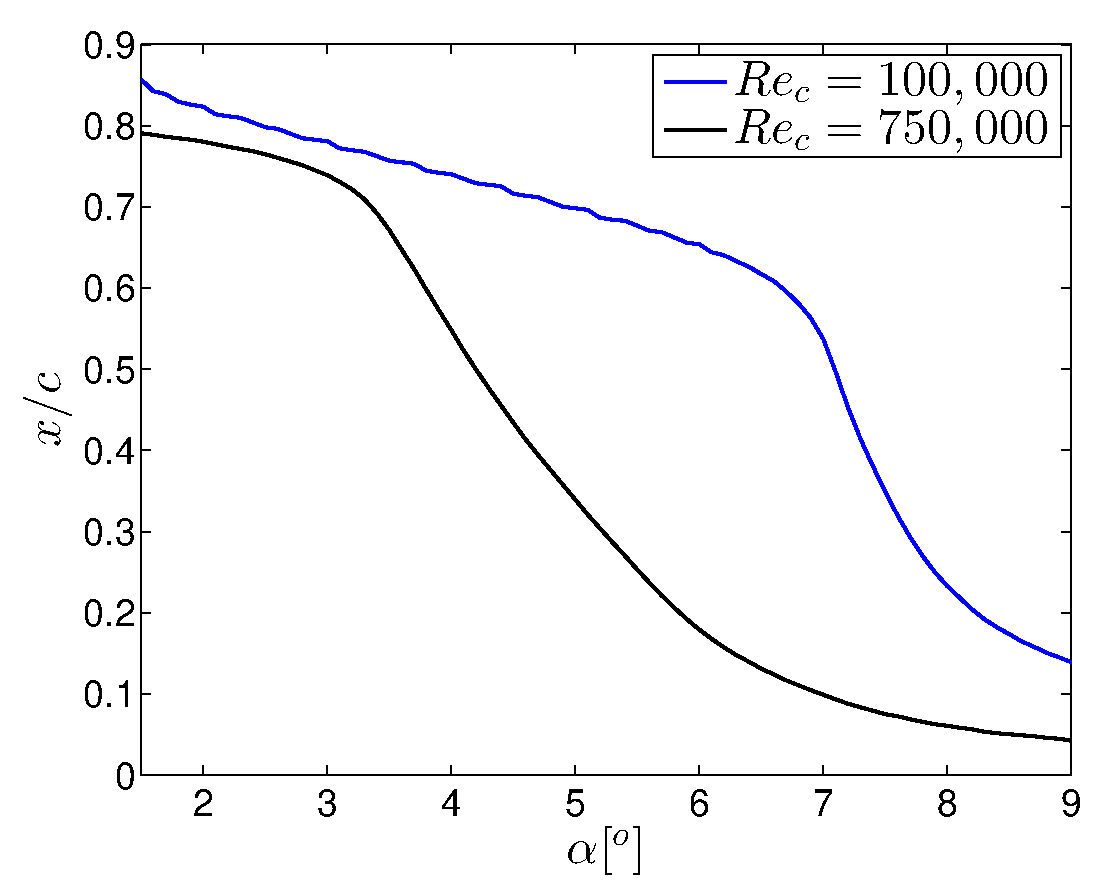
\includegraphics[width=1\textwidth]{tr_xfoil_100_750}
		\label{fig:tr_xfoil_100_750}		
	\end{subfigure}
	\begin{subfigure}[t]{0.45\textwidth}
		\caption{}
		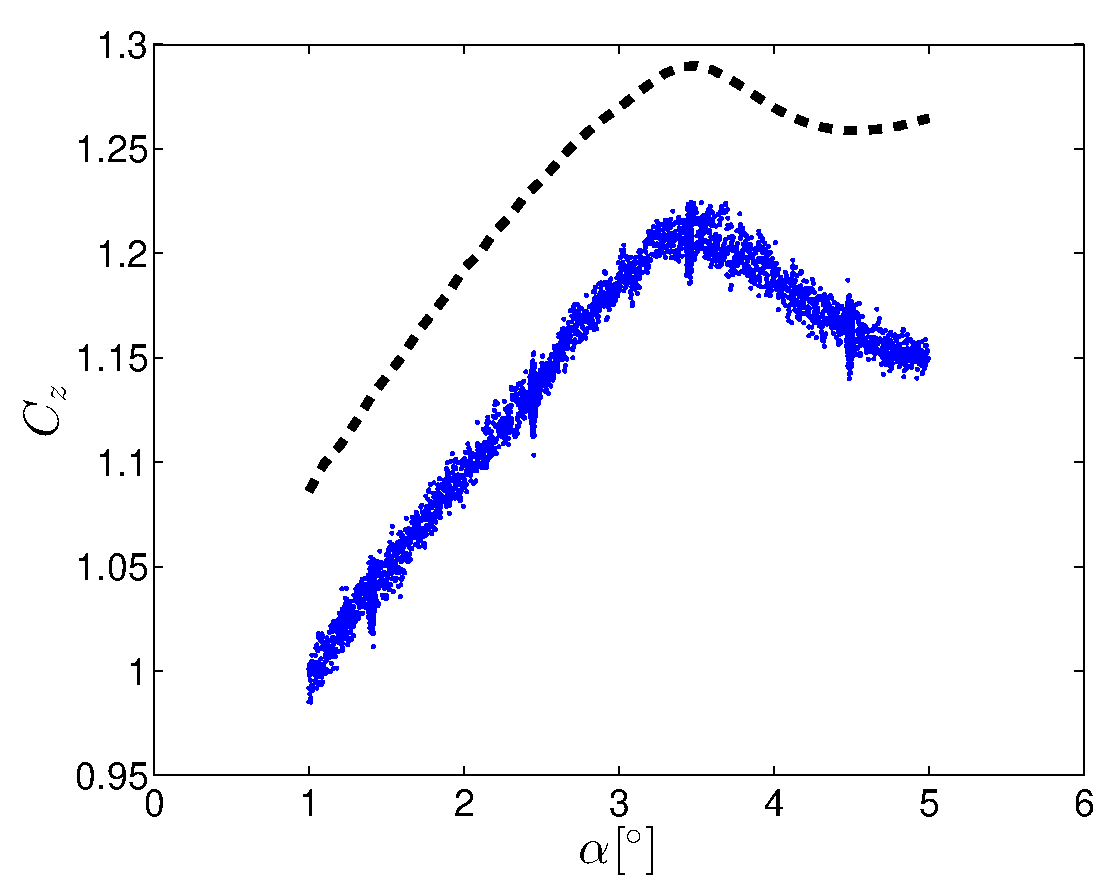
\includegraphics[width=1\textwidth]{765k_static_model_cz_xfoil}
		\label{fig:765k_static_cz_foil}
	\end{subfigure}
	\caption{(a) Transition location calculated using XFOIL for two different Reynolds numbers. (b) Normal force coefficient measured in experiments (dots) and from XFOIL calculations (dashed line) for $Re_{c}=750,000$.}		
\end{figure}
Numerical simulations are performed with stationary airfoils to ensure the expected static boundary layer characteristics are captured by the numerical simulations.  Figure~\ref{fig:overview_la2_750k_stationary} depicts the instantaneous vortical structures in the flow for $Re_{c}=750,000$ for an angle of attack $\alpha=2.4^{\circ}$ and $\alpha=4.4^{\circ}$ which shows the change in boundary layer characteristics in the static cases. Similarly, figure~\ref{fig:overview_isocontour_aoa} shows the static boundary layer characteristics for $Re_{c}=100,000$ at $\alpha=6.7^{\circ}$ and $\alpha=8.0^{\circ}$.
\begin{figure}[h]
	\centering
	\begin{subfigure}[t]{0.49\textwidth}
		\caption{$\alpha=2.4^{\circ}$}		
		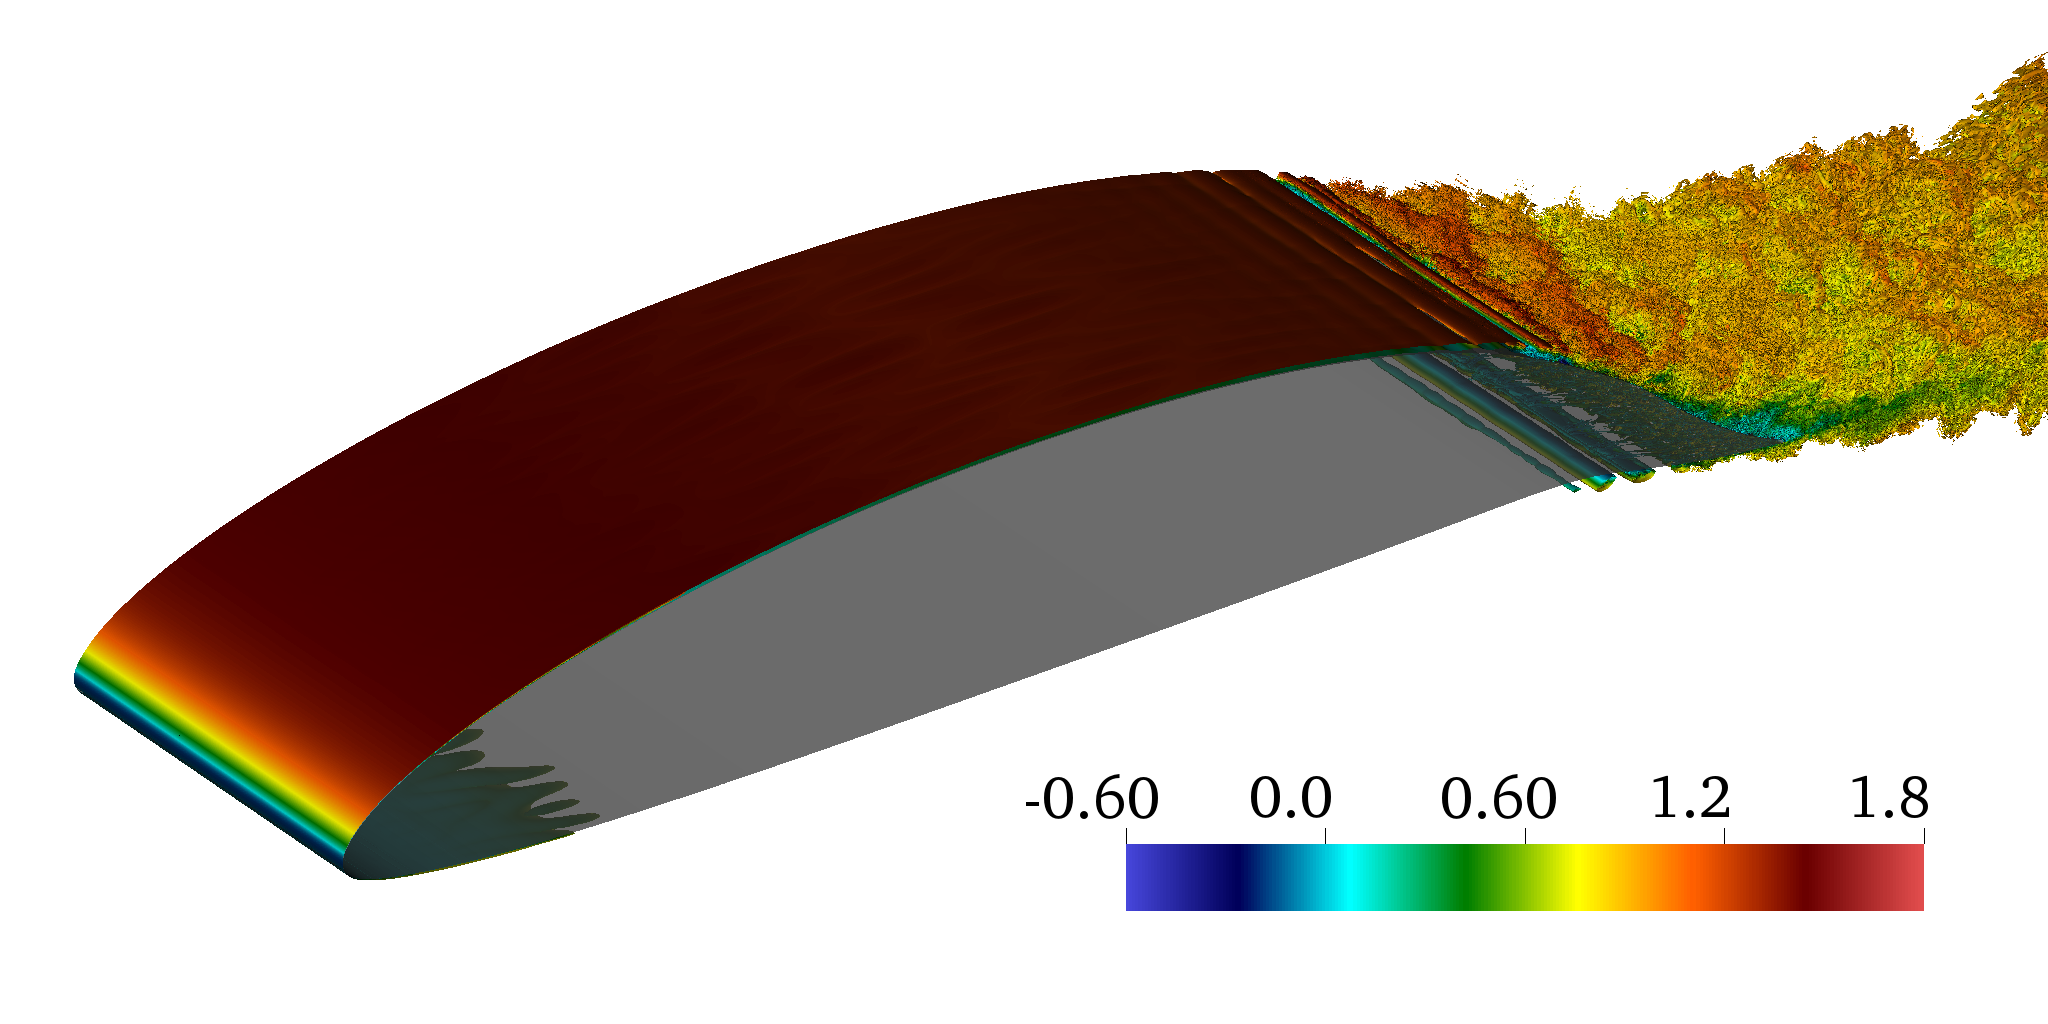
\includegraphics[width=1\textwidth]{paper2/imgs2/pitch_re750k0001}
		\label{fig:overview_la2_aoa24}
	\end{subfigure}
	\begin{subfigure}[t]{0.49\textwidth}
		\caption{$\alpha=4.4^{\circ}$}		
		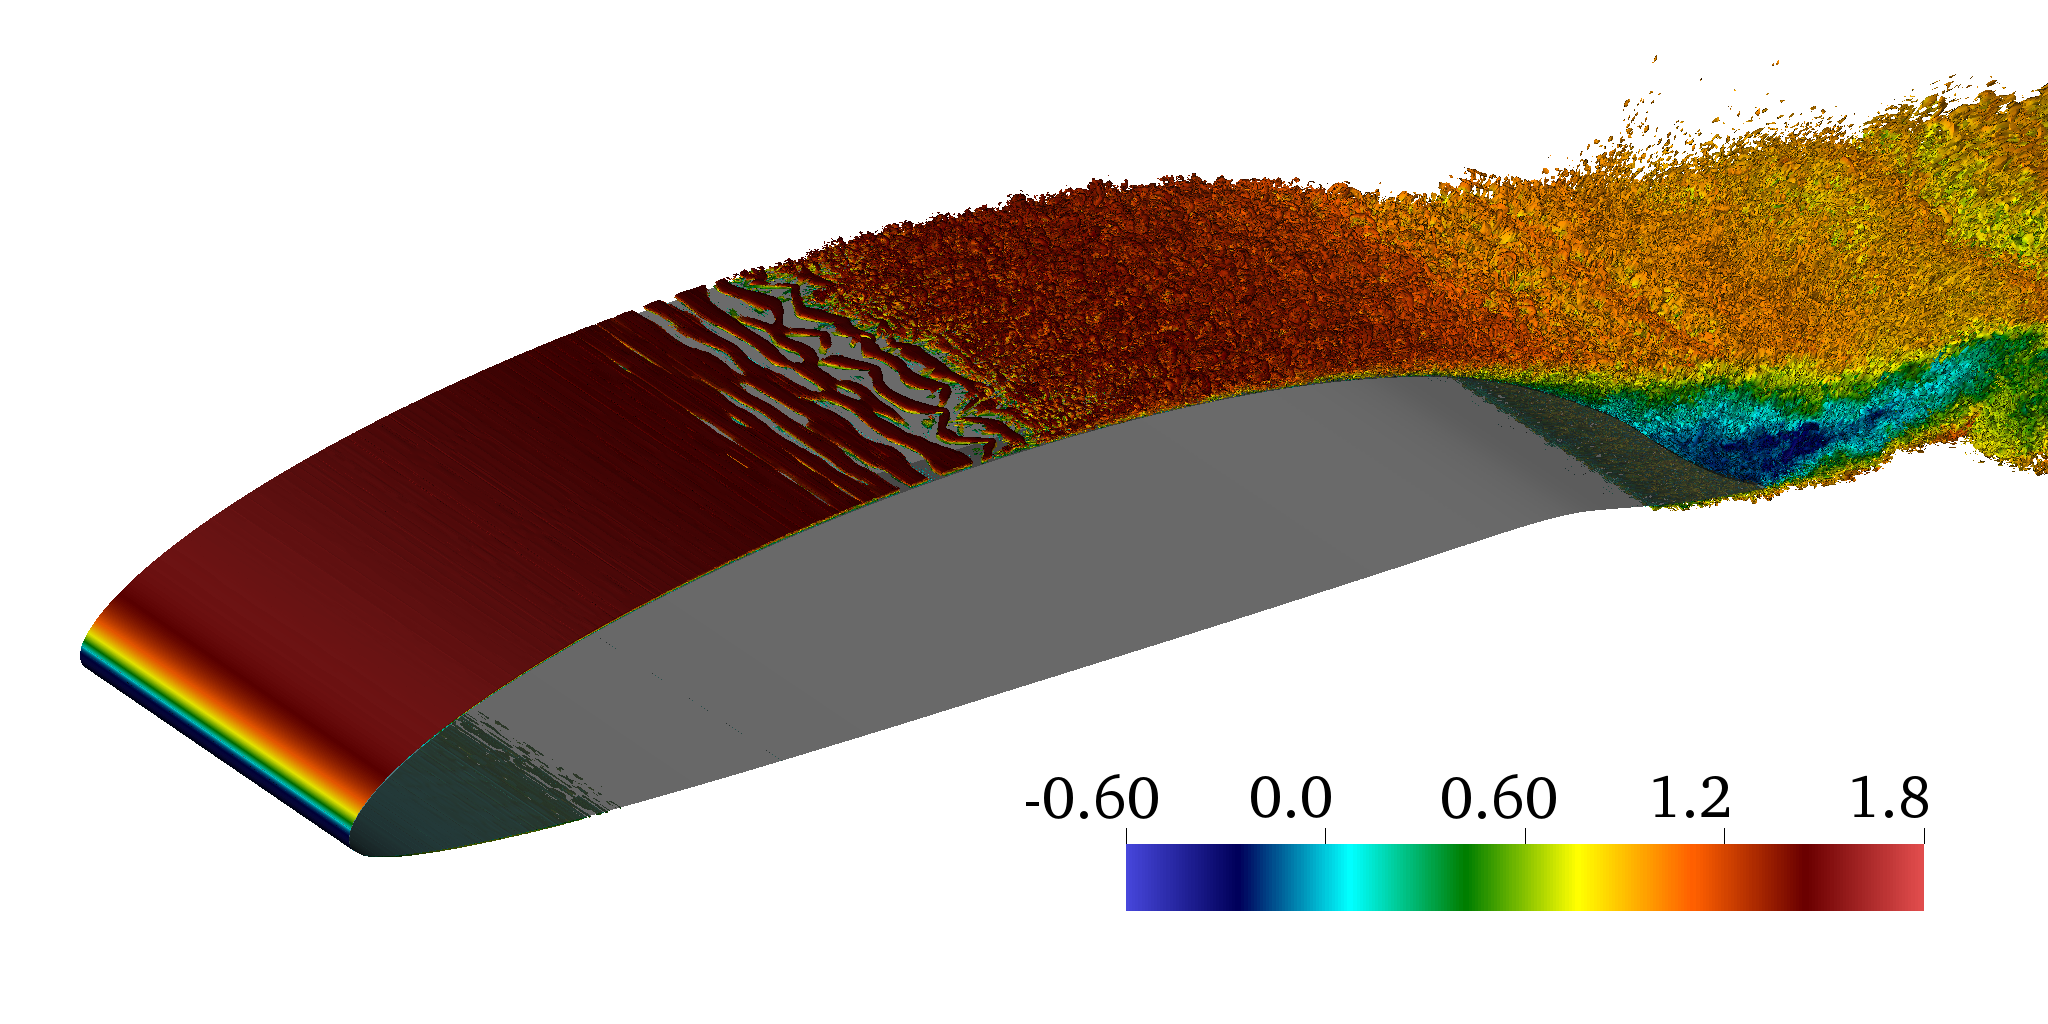
\includegraphics[width=1\textwidth]{paper2/imgs2/pitch_re750k0002}
		\label{fig:overview_la2_aoa44}		
	\end{subfigure}	
	\caption{Instantaneous vortical structures identified by the $\lambda_{2}$ criterion for the two stationary angle of attack simulations at $Re_{c}=750,000$.}
	\label{fig:overview_la2_750k_stationary}
\end{figure}

\begin{figure}[t]
	\begin{subfigure}[b]{0.49\textwidth}
		\centering
		\caption{$\alpha=6.7^{\circ}$}		
		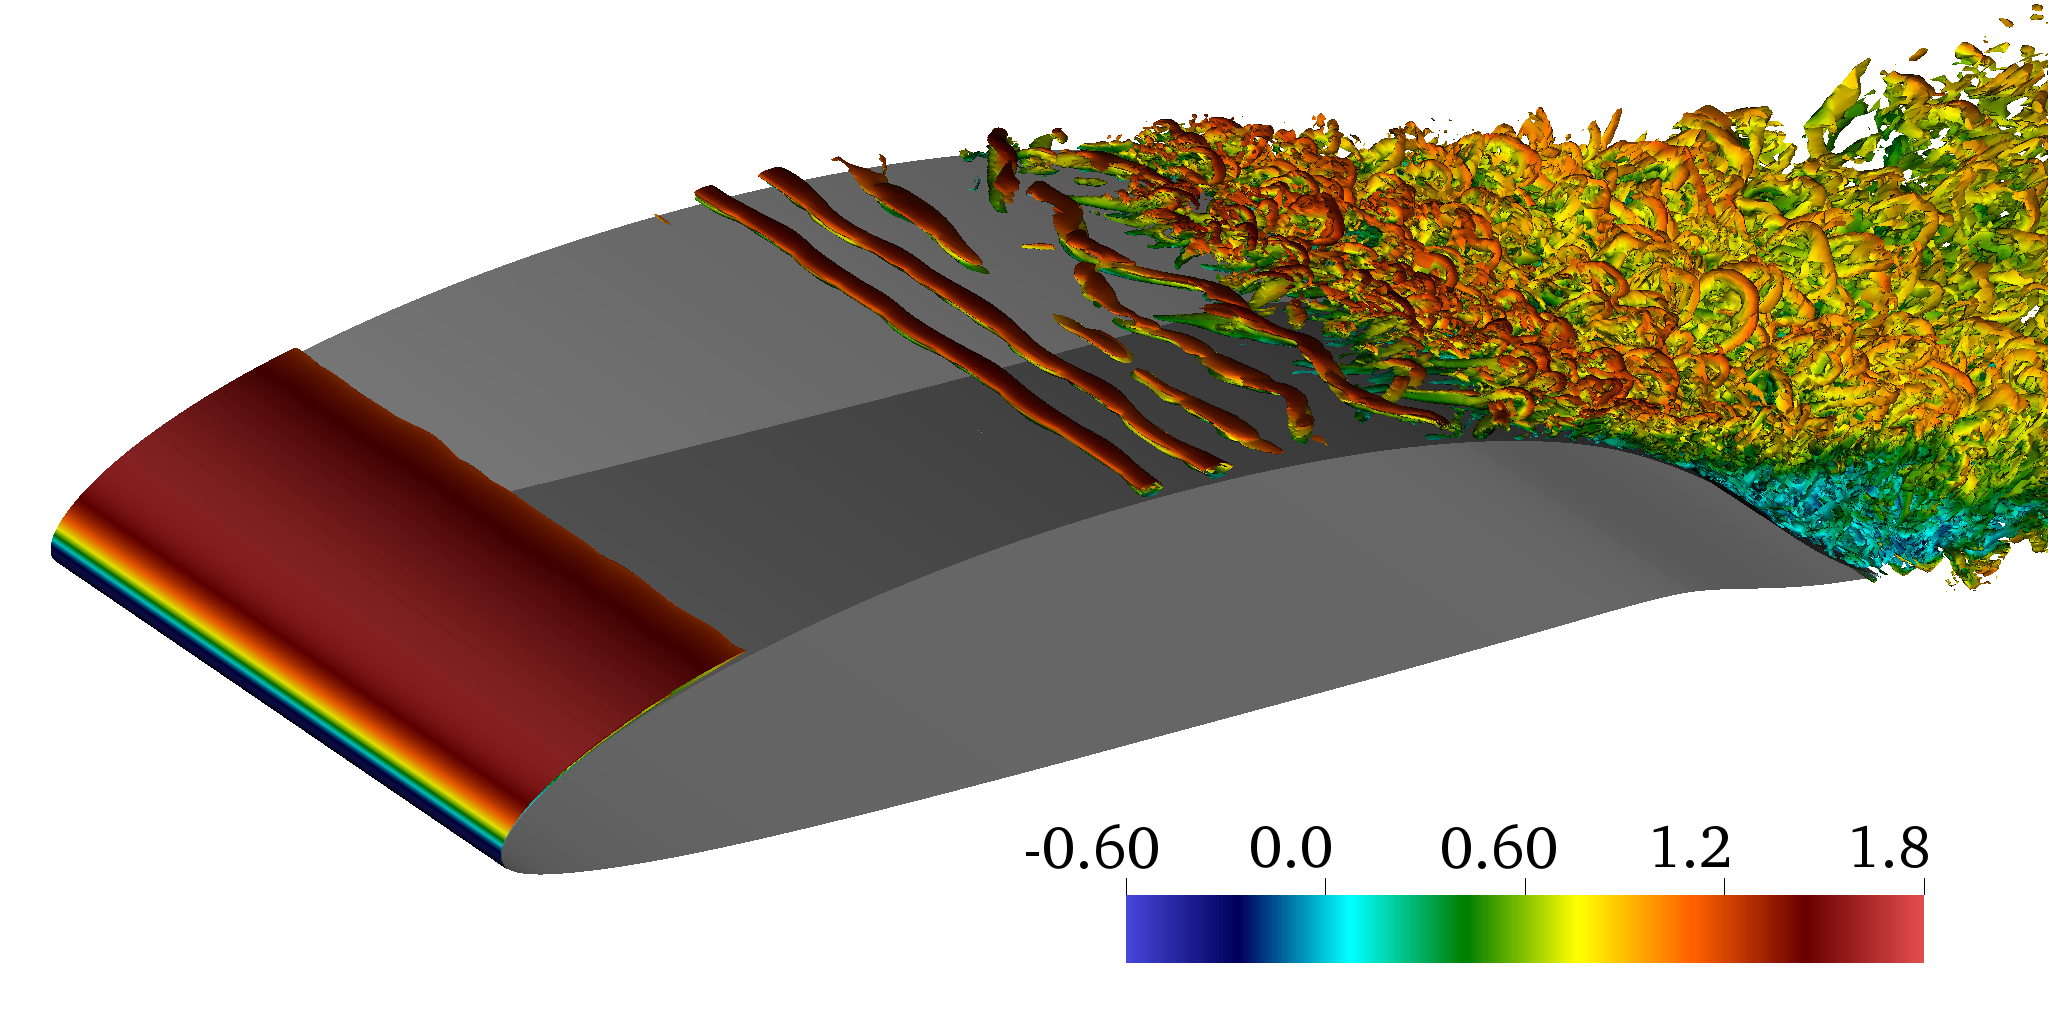
\includegraphics[width=1\textwidth]{paper3/imgs/re100k_static67_0001}
		\label{fig:overview_aoa67_iso}
	\end{subfigure}
	\begin{subfigure}[b]{0.49\textwidth}
		\centering
		\caption{$\alpha=8.0^{\circ}$}		
		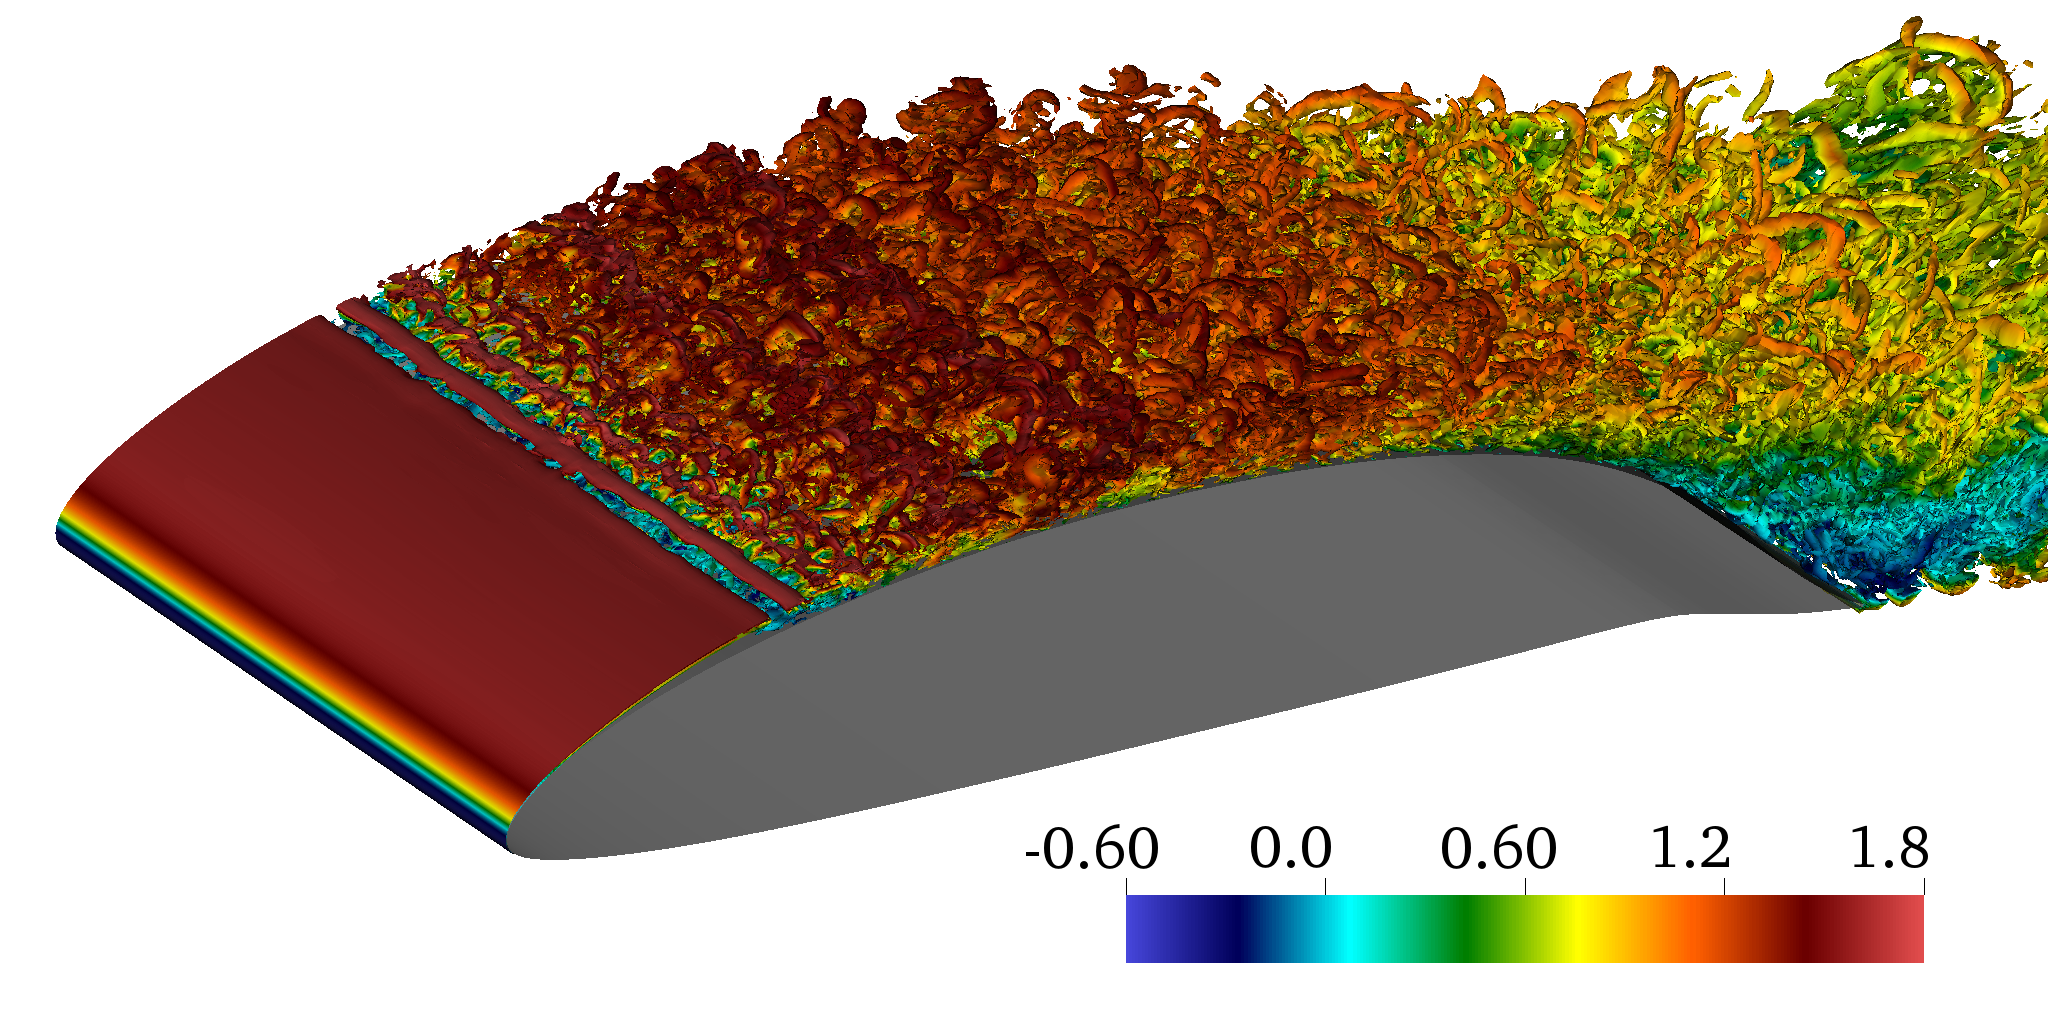
\includegraphics[width=1\textwidth]{paper3/imgs/re100k_static80_0001}
		\label{fig:overview_aoa80_iso}
	\end{subfigure}
	\caption{Isocontours of instantaneous $\lambda_{2}$ structures observed for two different (stationary) angles of attack at $Re_{c}=100,000$.}
	\label{fig:overview_isocontour_aoa}
\end{figure}

For both the Reynolds number cases, significant temporal variation of transition location is also found for the unsteady cases. Figure~\ref{fig:overview_transition_alpha} shows the variation of transition with respect to $\alpha$. The transition locations were calculated using thresholds on the instantaneous spanwise-averaged Reynolds stress $\overline{u'v'}$ and spanwise fluctuation intensity $\overline{w'w'}$. For the lower Reynolds number case the boundary layer also develops a leading-edge laminar separation bubble during the pitch cycle which significantly influences the boundary-layer dynamics.

\begin{figure}[t]
	\begin{subfigure}[b]{0.49\textwidth}
		\centering		
		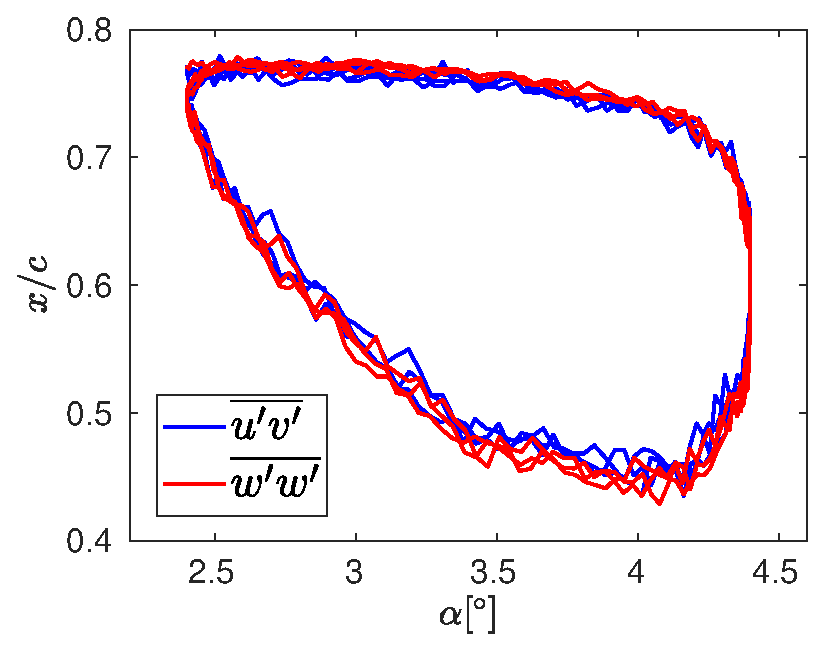
\includegraphics[width=1\textwidth,height=0.80\textwidth]{imgs/750k_transition_alpha.eps}
	\end{subfigure}
	\begin{subfigure}[b]{0.49\textwidth}
		\centering	
		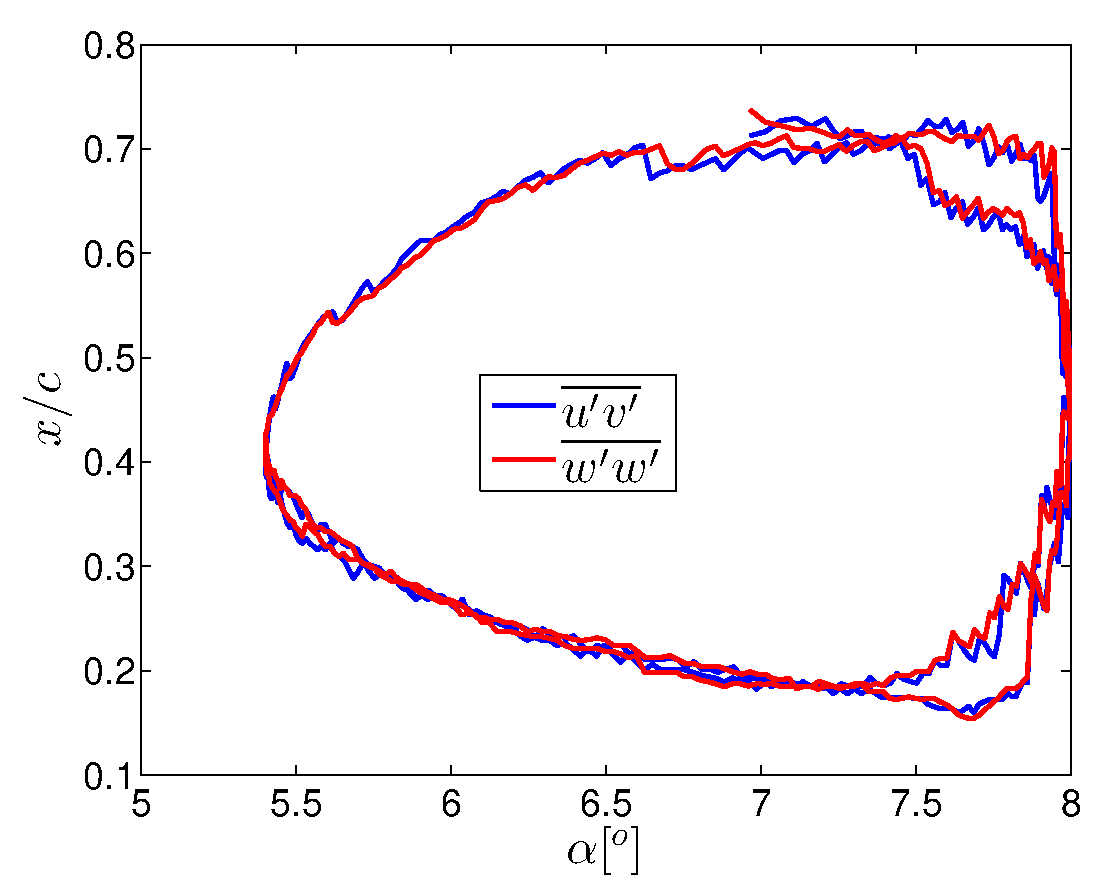
\includegraphics[width=1\textwidth]{paper3/imgs/transition_alpha.eps}
	\end{subfigure}
	\caption{Phase portraits of transition location for (left) $Re_{c}=750,000$ and (right) $Re_{c}=100,000$.}
	\label{fig:overview_transition_alpha}
\end{figure}


\section{Flow around a stationary wing section}

The final paper in the thesis deals with the study of the boundary layer over a wing section at a chord-based Reynolds number of $Re_{c}=1,000,000$. The airfoil used for the study is the asymmetric NACA 4412. A DNS database for the flow around the same airfoil at $Re_{c}=400,000$ is available and comparisons are made between the two cases to assess the effects of changing Reynolds number on the developing boundary layer. The numerical setup is done in a manner very similar to the computational study by \cite{hosseini16}. Figure~\ref{fig:overview_flow_field_re1000k} shows a section of the numerical grid and the instantaneous vortical structures in the flow field. Figure~\ref{fig:overview_beta_Reth_Ret} shows a comparison of the different measures of the boundary layer over the chord-wise distance for the two different Reynolds numbers. While both wall-shear stress (indicated by $Re_{\tau}$) and boundary layer thickness (measured with momentum thickness Reynolds number $Re_{\theta}$) change between the two cases, the Clauser parameter stays nearly the same throughout the chord. This allows comparisons across different Renolds numbers without ambiguity since the pressure gradient histories remain the same with changing Reynolds numbers. 
\begin{figure}[t]
	\centering
	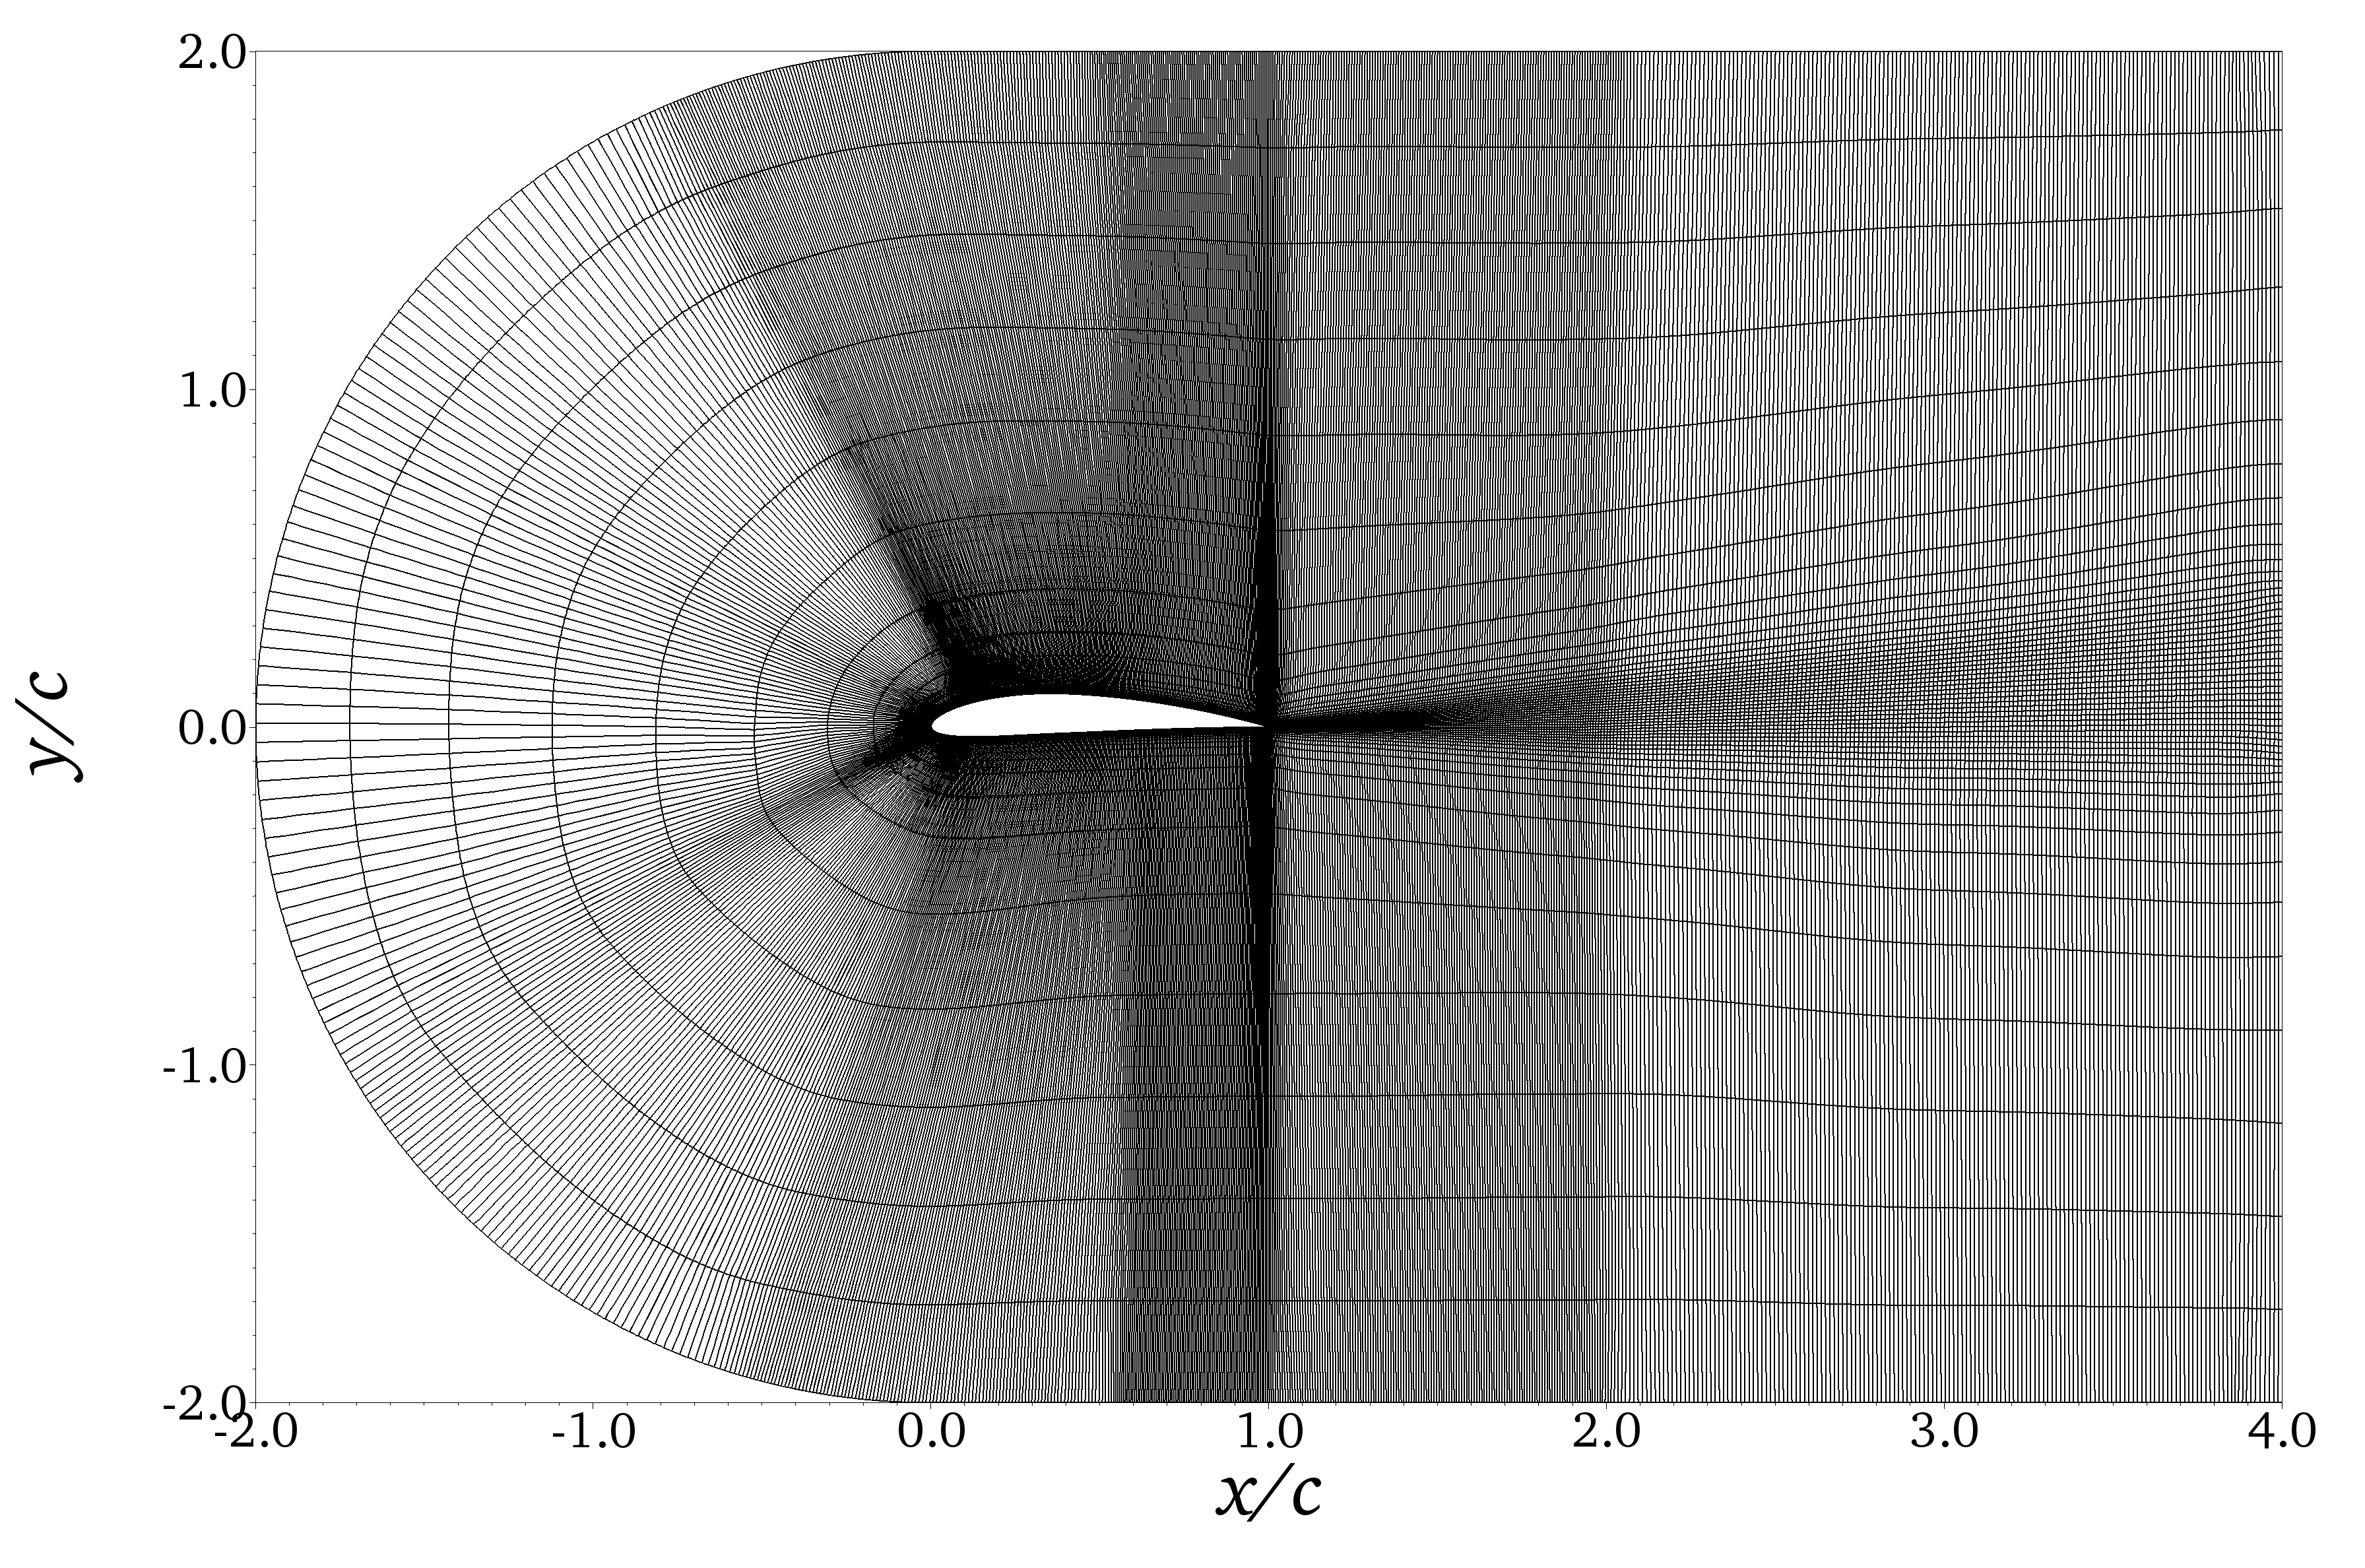
\includegraphics[width=0.49\textwidth]{paper4/imgs/wing_mesh}
	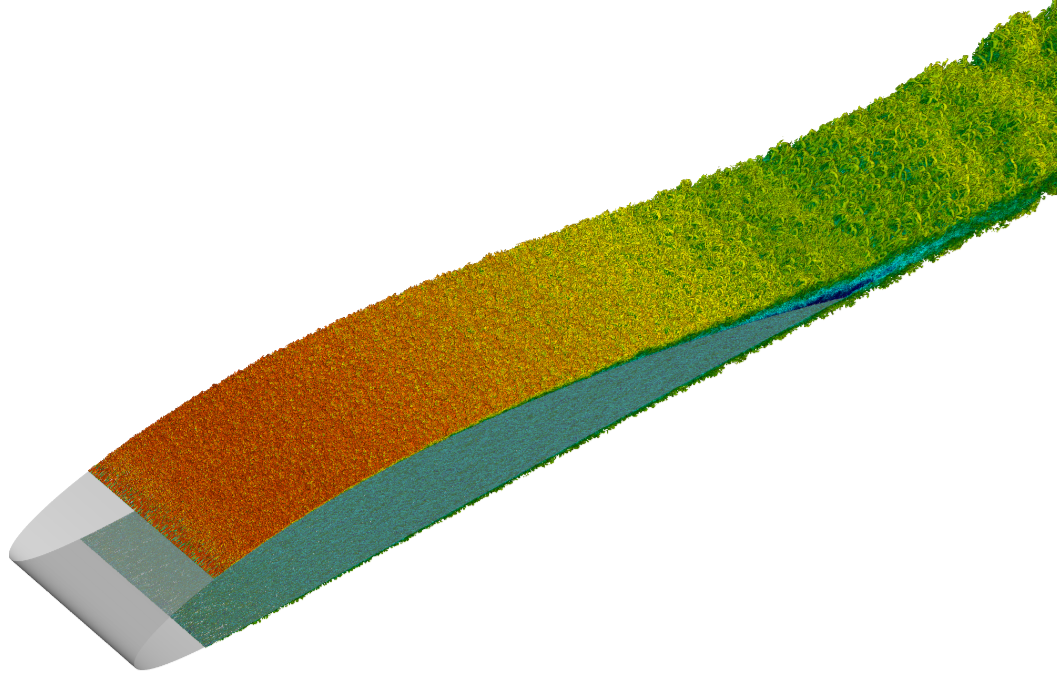
\includegraphics[width=0.49\textwidth]{paper4/imgs/wing_visualization}
	\caption{(Left) Two-dimensional slice of the computational domain showing the spectral-element distribution. (Right) Instantaneous flow field showing coherent structures identified with the $\lambda_{2}$ method \citep{jeong95}, and colored with horizontal velocity. In this figure, dark blue represents a horizontal velocity of $-0.1$ and dark red a value of $2$.}
	\label{fig:overview_flow_field_re1000k}
\end{figure}

\begin{figure}[t]
	\centering
	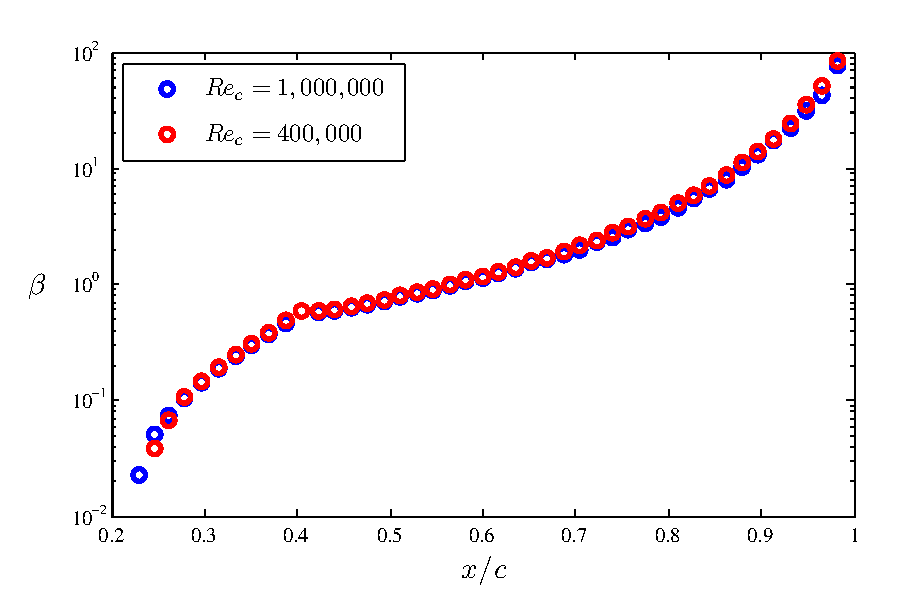
\includegraphics[width=0.49\textwidth]{paper4/imgs/beta_vs_x}
	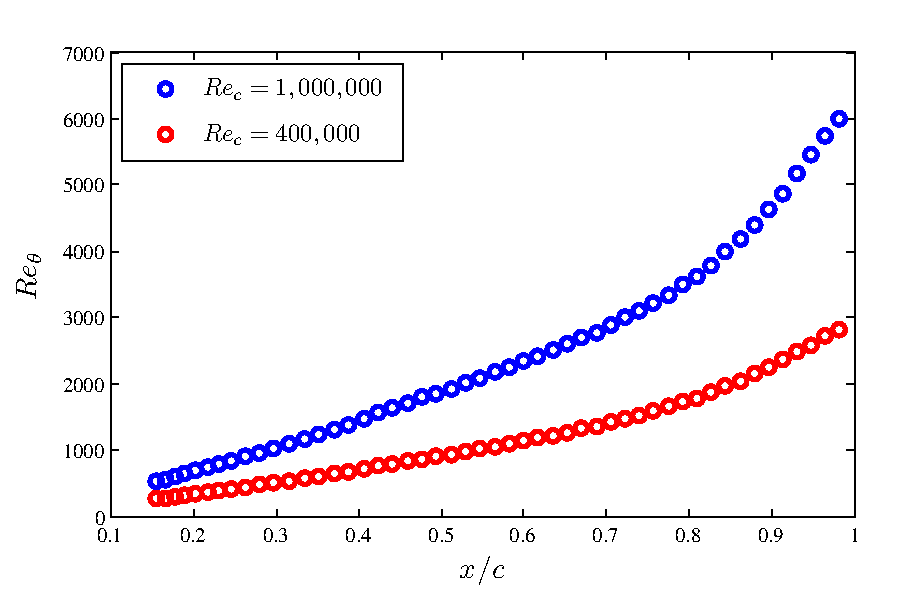
\includegraphics[width=0.49\textwidth]{paper4/imgs/Reth_vs_x}
	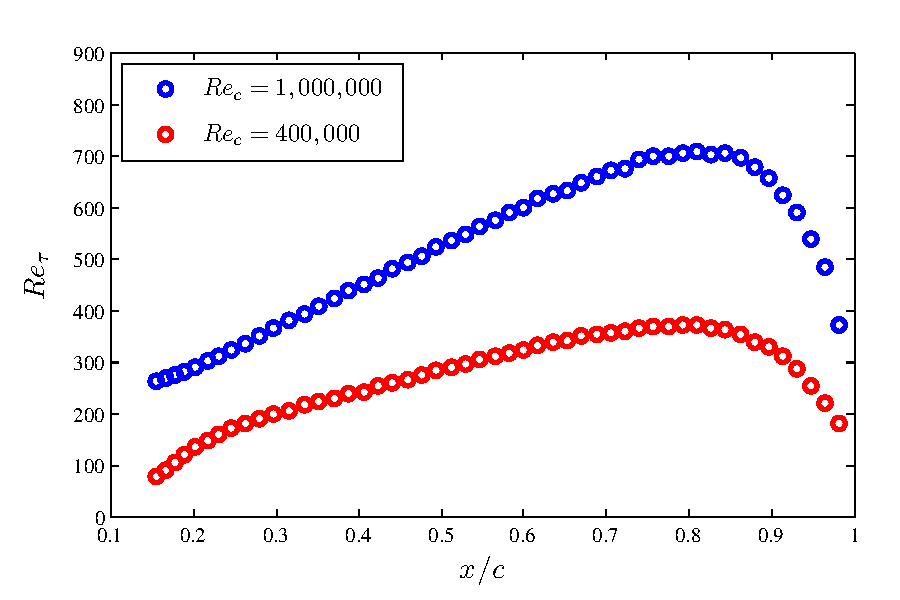
\includegraphics[width=0.49\textwidth]{paper4/imgs/Ret_vs_x}
	\caption{Streamwise evolution of (top left) the Clauser pressure-gradient parameter $\beta$, (top right) the Reynolds number based on momentum thickness $Re_{\theta}$ and (bottom) the friction Reynolds number $Re_{\tau}$, for the two wing cases under study.}
	\label{fig:overview_beta_Reth_Ret}
\end{figure}

%===============================================================================
\chapter{Conclusions and outlook}
%===============================================================================

The current thesis work concerns three different fields of research.

In the first part of the thesis, the ``evolve and filter'' technique for the stabilization of spectral-element methods is analyzed and it is found the filter operation causes an undesirable loss of divergence-free quality of the solution. This loss of divergence is shown to be particularly large for the test case of a double shear layer. An alternate formulation of the stabilization called the relaxation-term (RT) stabilization is shown to overcome the drawbacks of the explicit filtering technique, while maintaining the simplicity of the original explicit filter. This RT stabilization technique is very closely related to explicit filtering, with the two operations being equivalent to the leading order in time. Stability limits of the RT stabilization are explored and is shown to be stable within the practical parameter range.

In the second part, an NLF airfoil undergoing small-amplitude pitch-oscillations is analyzed at two different Reynolds numbers. In both cases a large variation of transition, and thus boundary layer characteristics is observed over the airfoil resulting in a non-linear response of the aerodynamic force coefficients. For $Re_{c}=750,000$ it shown that the temporal evolution of the transition point can be understood with a simple phase-lag concept, with the implication that boundary-layer evolution may be considered quasi-steady in time. Using this phase-lag concept a simple empirical model is developed which is able to explain a fairly wide range of experimental data.

On the other hand, for $Re_{c}=100,000$ a qualitatively different picture emerges for the unsteady boundary layer. The boundary-layer response displays a dynamically rich behavior with marked asymmetry of upstream and downstream transition movement. In this case, transition location is governed by the properties of the leading-edge laminar separation bubble (LSB) and it is conjectured that the absolute instability of the LSB may be responsible for abrupt changes in boundary layer characteristics.

Finally, in the third part of the study, flow over a stationary NACA 4412 airfoil is studied at two different Reynolds numbers with the aim of better understanding the boundary-layer evolution in non-equilibrium pressure gradient boundary layers. Two flow cases at a chord-based Reynolds number of $Re_{c}=400,000$ and $Re_{c}=1,000,000$ are compared at different streamwise locations. It is found that the effect of the streamwise pressure gradients is higher at low Reynolds numbers, leading to greater energy in the larger structures present in the outer part of the turbulent boundary layer.

The current work has laid the foundation for several interesting questions that may be the focus of future work. Can the simple empirical aerodynamic model be extended for a wider range of unsteady motions? Can the phase-lag be predicted a-priori as in the case of the classical model by \cite{theodorsen35}? When does the quasi-steady assumption break down and the boundary layer becomes truly unsteady? For $Re_{c}=100,000$, can the asymmetry of the (upstream and downstream) velocities of transition point be linked with the stability properties of the LSB? What is the influence of free-stream turbulence on unsteady LSB? In stationary airfoils, how does the velocity spectrum change with Reynolds number in non-equilibrium flows? What are the characteristics of boundary layer streaks in non-equilibrium flows? Some of these questions will be the focus of further research.


%===============================================================================
% Acknowledgments
%===============================================================================
%


\begin{acknowledgements}
	My foremost gratitude goes to my supervisor Dan Henningson for giving me the opportunity to join his research group. His knowledge and guidance have helped me immensely as a student. His encouragement, for which there is no substitute, have always provided the inspiration I needed to constantly push myself further in my work. Next I would like to thank my co-advisors Philipp Schlatter and Ardeshir Hanifi. Philipp for his patience during all my ignorant and sometimes foolish questions on numerics, conferences, papers and others that I probably can't recall. Ardeshir for the laughter, the sandwiches, the beers and most importantly, always being available on short notice when I needed help. I would also like to thank the members of the NFFP project, Roger Larsson, Dr. David Eller and Dr. Mikaela Lokatt for all the interesting discussions on aerodynamics. 
	
	I am grateful to Adam Peplinski for all the help he provided with Nek5000, MPI and coding in general. I can not imagine figuring out the workings of Nek5000 without his support. Armin and Ricardo have helped me more than others during my crucial time as a new Phd student. The help is greatly appreciated.
	
	Special mentions go to Mattias for all the coffee breaks, introducing me to Swedish food, the spontaneous discussions and being the bouncing board for all my (mostly wrong) ideas. Your company shall be missed once you leave the department. Jacopo and Giandomenico for all the great company, joining for the spontaneous plans and granting me the honorary Italian citizenship. I'll learn Italian very soon I promise! Marco for the constant dinner company. Freddy for the weekend food+beer+movie routine. Elektra for being one of the greatest friends of all time. Politics, late-night and of course Trump shall keep us entertained for times to come. But mostly, thanks for correcting my manuscripts and the support during this licentiate period. A mention must also go to my unrequited love, Walter Fornari. Where will I find another like you?
	
	A hearty thanks goes out to all my friends here at the department who make this a wonderful place. Eric, Clio, Nicolas, Sudhakar, Ugis, Evelyn, Anthony, Mehdi, Ali, Guillaume, Luca, Luca, Pierluigi, enrico, Francesco, Kristina, Ekatrina, J.C., Matthias, Priti, Ninge, Sagar, Krishne, Dhiya, and everyone else. All of you, with your quirks, jokes, stories and gossip (looking at you Pierluigi) add a little bit of color to life everyday.
	
	Perhaps most importantly, my deepest gratitude goes towards my family for their patience, unconditional love and support during my ever wandering path through life.
	
	Lastly, financial support for this work was provided by Vinnova through the NFFP project UMTAPS, with grant number 2014-00933, the Knut and Alice Wallenberg Foundation, and the European Research Council under grant agreement 694452-TRANSEP-ERC-2015-AdG.\ The computations were performed on resources provided by the Swedish National Infrastructure for Computing (SNIC) at the PDC Center for High Performance Computing at the Royal Institute of Technology (KTH). Simulation have also been performed at the Barcelona Supercomputing Center, Barcelona, with computer time provided by the $12^{th}$ PRACE Project Access Call (number 2015133182) and at the High Performance Computing Center, Stuttgart (HLRS) with the computer time provided by the $15^{th}$ PRACE Project Access Call (number 2016163965). 

\end{acknowledgements}



%===============================================================================
% References
%===============================================================================
%
\bibliographystyle{jfm}
\bibliography{licentiate}
%
\IfFileExists{overview.bbl}{\graphicspath{{imgs/}}
%\setlength{\captionmargin}{50pt}

%===============================================================================
\chapter{Introduction}
%===============================================================================
\section{A short history}

The first sustained flight by the Wright brothers in 1903 marked a historic day in human achievement and ingenuity. Momentous as the achievement was, the Wright brothers did not truly invent the modern airplane. Their achievements were the fruition of nearly a century of aeronautical research, starting perhaps with Sir George Cayley, who is considered the ``father of aerial navigation'' \citep{gibbs-smith62}. The principal components of the modern aircraft were laid down by George Cayley as early as 1799. Prior to Cayley, the ideas for mechanical flight tended towards flapping wings, where the flapping motion produced both propulsion and lift. George Cayley was the first to break the unsuccessful chain of thought and separated the two aspects of flight into distinct systems. His triple paper ``On Aerial Navigation'' published in Nicholason's \textit{Journal of Natural Philosophy, Chemistry and the Arts} on November 1809, February and March 1810 \citep{cayley1809} mark some of the most important works in aeronautical history. In the works, Cayley states for the first time, the principle of lift generation \textit{i.e.} the formation of a low pressure region on the upper surface of the wing. His paper elaborates on the separation of lift from propulsion and also goes on to talk about flight control and airplane stability. Later in his life, he proposed the concept of multiplanes (multiple wings mounted on top of each other) and built the first glider triplane named the ``boy carrier'' in 1849.

Several investigators followed the quest of ``aerial navigation''. Otto Lilienthal was the first to design and successfully fly controlled gliders in 1891, going on to make over $2500$ successful glider flights. Octave Chanute brought aeronautics research to America and designed a biplane glider which directly inspired the designs of the Wright Brothers. Samuel Pierpont Langley was a contemporary of the Wright brothers who built and tested several powered model airplanes. His success in achieving powered flight directly influenced and encouraged the Wright brothers. The final historic achievement of successful powered flight was achieved by the Wright brothers. On December $17^{th}$ 1903, a gasoline powered biplane by the name Wright Flyer I (figure~\ref{fig:wright_flight}) took flight in (modern day) Kill Devil Hills, North Carolina, ushering forth the era of practical human flight.
\begin{figure}[h]
	\centering
	\includegraphics[width=0.90\textwidth]{wright_brothers_first_flight}
	\vspace{10pt}	
	\caption{First flight of the Wright Flyer I, December 17, 1903, Orville piloting, Wilbur running at wingtip. Image from \cite{wikipedia_wright}.}
	\label{fig:wright_flight}
\end{figure}

\section{Modern aircraft design}
Since that fateful day, modern airplanes have been used in a variety of different conditions, varying from commercial passenger planes, to supersonic military aircrafts \citep{blackbird}, 
to endurance flights around the world lasting 9 days \citep{rutan_voyager}. The myriad uses have resulted in various challenges that need to be overcome by the aircraft designers. One significant challenge has been due to the dynamic interaction of air flow with the airplane structures, now studied under the field of aeroelasticity. These problems came to the fore as the design speed of aircrafts increased over the years and designers came to favor monoplanes over the biplane design. An early example was that of the Fokker D-8 German aircraft during World War I which suffered wing failure under steep dives, which was the first documented case of static aeroelastic effects.

Today the designers of commercial aircrafts face another challenge brought about by global climate change and rising oil prices. With the realization of the contribution of the aviation industry towards global climate change \citep{green08}, aircraft designers now face a need to significantly improve the fuel efficiency of commercial aircrafts in a bid to reduce the carbon footprint of the industry. In an effort to quantify the opportunities of achieving such an improvement, \cite{schrauf05} showed a break-down of the drag experienced by a typical transport aircraft highlighting that frictional drag accounted for more than half the drag experienced by the aircraft. Clearly a favorable modulation of the boundary layer over the wing could help achieve large improvements in fuel efficiency. The modulation could come in the form of effective flow control strategies, or with wing design strategies such as the use of natural laminar flow (NLF) airfoils. Both \cite{schrauf05} and \cite{green08} push forward the idea that NLF airfoils and laminar flow control strategies are the low-hanging fruits in the goal of higher fuel efficiency and a concerted effort into addressing the engineering challenges for practical implementation must be made. Some of these challenges may require revisiting the aeroelasticity problems from the perspective of laminar wings. However laminar flow at high Reynolds numbers is susceptible to destabilization and may not always be possible. Thus turbulent drag reduction strategies need to be used effectively where needed \citep{bushnell03}. Whatever the form of drag reduction technique that may finally be implemented on a particular aircraft, the understanding of developing boundary layers over wings (including the influence of control strategies) occupies a central position in aerodynamic research if the goal of higher fuel efficiency is to be realized. With this goal in mind, the current thesis work aims to further the understanding of developing boundary layers over airplane wings, focusing on two particular aspects.
\begin{itemize}
	\item Understanding the structure of the turbulent boundary layer developing over a wing section.	
	\item Understanding the evolution of the developing boundary layer over a natural laminar flow airfoil in unsteady flight conditions. 
\end{itemize}

%Solutions to these emerging aeroelastic problems needed an understanding of the unsteady phenomenon occurring in practical flight conditions. Such understanding came via the works of \cite{glauert30,karman38,theodorsen35} \textit{etc}, and by the 1940s, design engineers had the tools to account for unsteady aeroelastic effects in their wing designs.

%The achievements of these early aerdynamicists is quite impressive in particular considering that the boundary layer concept was in its nascent stages when the first practical airplanes were being designed. Indeed Prandtl's revolutionary concept of a boundary layer was first presented in 1904, almost a full year after the first flight of the Wright brothers.  

%-------------------------------------------------------------------------------
\section{Boundary layers over a stationary wing}

The understanding of the structure and scaling of wall-bounded turbulent flows has been in study for several decades and a complete understanding still remains far from complete. These flows have been studied with different canonical geometries such as channels \citep{kim87,moser99,lee15}, pipes \citep{elkhoury13,jimenez08,chin15} and flat plates \cite{spalart88,schlatter10,eitel14}. For the case of spatially evolving boundary layers over a flat plate, the simplest canonical case involves boundary-layer evolution subjected to a zero pressure gradient (ZPG). These flows may be uniquely characterized by a single parameter, \textit{i.e.} the Reynolds number Re, which is the ratio of the inertial and viscous scales of the flow. However practical flow cases are often influenced by pressure gradients. Such flow cases can no longer be uniquely defined using a single parameter. \cite{clauser54} with intuitive reasoning proposed a concept of an equilibrium boundary layer which may be uniquely defined by two parameters. He argued that, if the ratio of the average pressure gradient force across the boundary layer and the viscous shear force at the wall remains constant, the boundary layer would experience a similar flow history throughout its evolution. Thus the equilibrium pressure gradient boundary layers are uniquely defined by two parameters, namely the Reynolds number (Re) and the pressure gradient parameter $\beta$, defined as
\begin{eqnarray}
	\beta = \delta^{*}(dp/dx)/\tau_{w},
\end{eqnarray}
where $\delta^{*}$ is the displacement thickness, $dp/dx$ is the pressure gradient and $\tau_{w}$ is the wall-shear stress. The parameter is commonly referred to as the Clauser parameter. A flow case with a spatially constant Clauser parameter is categorized as an equilibrium boundary layer and a ZPG boundary layer is a special case of an equilibrium boundary layer with $\beta=0$. Several works have focused on pressure gradient boundary layers ranging from theoretical studies by \cite{townsend56,townsend56b,mellor66}, experimental works of \cite{skare94,harun13} and numerical simulations by \cite{spalart93,skote98}. The developing boundary layer over an airfoil however further increases in complexity since these boundary layers fall under the category of non-equilibrium boundary layers where the Clauser parameter is spatially varying. In such cases the flow history also plays a role in determining the local boundary layer properties \citep{clauser54,bobke17}. Analysis of such flow cases becomes significantly more difficult since the local boundary layer parameters do not uniquely define the state of the boundary layer. Nonetheless the study of such boundary layers is important since generic boundary layers found in nature would belong to this category, including the boundary layers over wings. The boundary layer developing over the NACA 4412 airfoil has the property that the spatially varying Clauser parameter is insensitive to Reynolds number. The presents us with the opportunity to study the Reynolds number effects of a non-equilibrium boundary layer with a constant pressure gradient history. That is indeed the methodology followed in this work. The developing boundary layer over a NACA 4412 wing section is analyzed at two different Reynolds numbers in order to understand Reynolds number effects in non-equilibrium boundary layers.

\section{Unsteady boundary layers}
%
Unsteady aeroydnamic studies started with the emergence of aeroelastic phenomenon in the early part of the $20^{th}$ century. With the gradual shift to monoplane designs, the inherent high torsional stiffness of biplanes was lost and aerodynamic instabilities, such as the one experienced by the Fokker D-8 became important. Pioneering works of \cite{glauert30,karman38,theodorsen35} \textit{etc}, provided the insight and modeling of such unsteady aerodynamic behavior and by the 1940s the foundations of unsteady aerodynamics for incompressible attached flows had been laid down. The mathematical framework these unsteady aerodynamic theories relied on simple inviscid and quasi-steady assumptions, which proved to be highly attractive to the wing designers \citep{leishman00}. Experimental corroboration by \cite{halfman52} and \cite{rainey57} further added support to the validity of the simple assumptions. Over the next few decades, investigations of unsteady aerodynamics shifted focus to the understanding of the dynamic stall phenomenon, with works of \cite{mccroskey76,mccroskey81,mccroskey82experimental,mccroskey82,carr1977,crisler94}. A large body of work on unsteady separated flows was presented by \cite{ericsson86,ericsson87b,ericsson_stall88a,ericsson_stall88b}. The studies continue to this day with the works of \cite{visbal11,visbal14,visbal17,dunne2015} and several other authors, a recent review can be found in \cite{coorke15}. 
\begin{figure}[h]
	\centering
	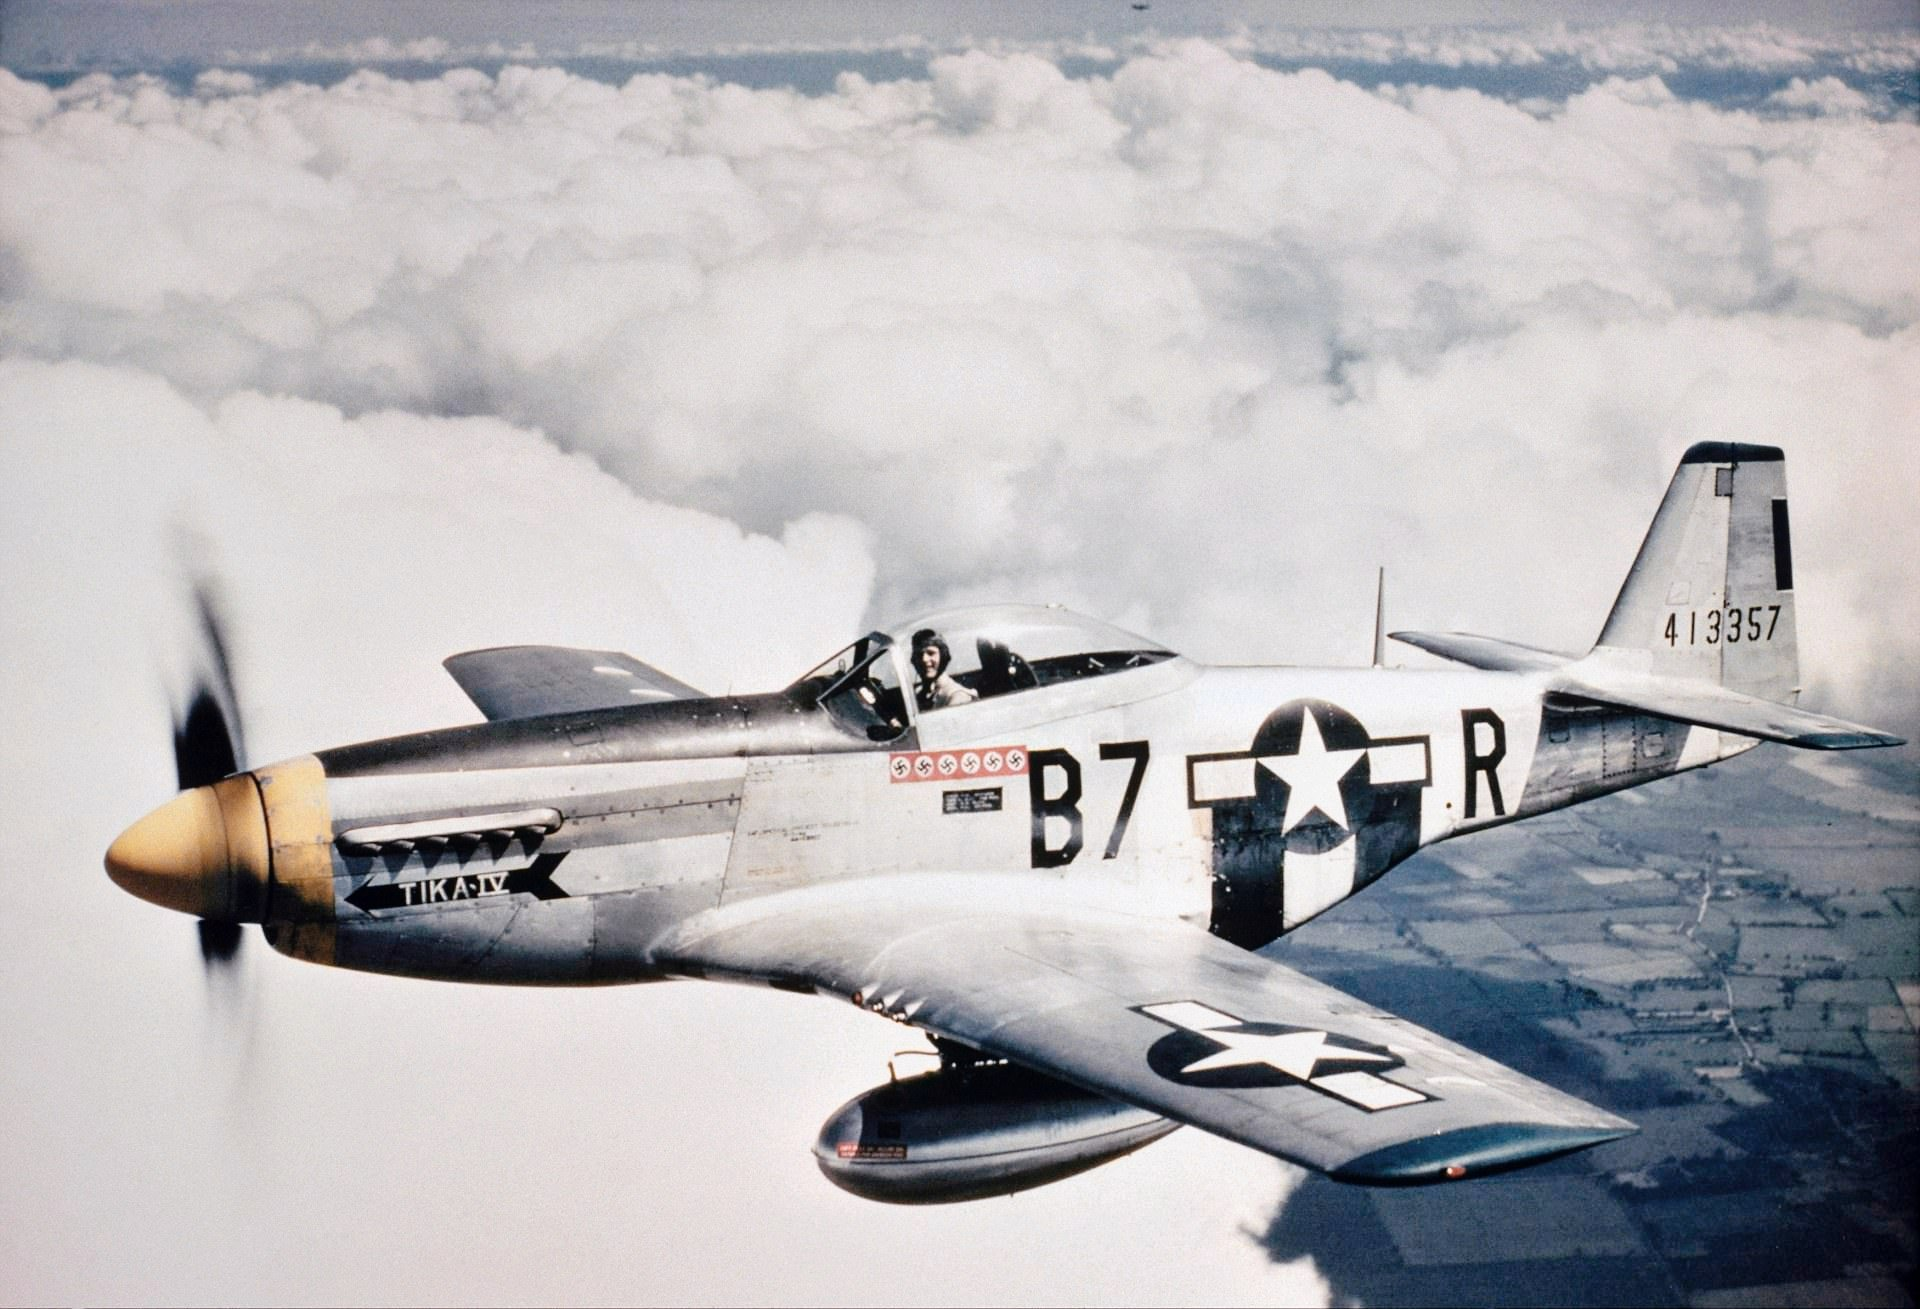
\includegraphics[width=0.90\textwidth]{P-51-mustang}
	\vspace{10pt}
	\caption{North American P-51 Mustang. Image from \cite{wikipedia_mustang}.}
	\label{fig:mustang}
\end{figure}

However it appears that the aeroelasticity problem was not considered from the perspective of natural laminar flow airfoils. This is a surprising fact considering the P-51 Mustang (figure~\ref{fig:mustang}), a fighter aircraft in the Royal Air Force designed in 1940, incorporated a wing with a natural laminar flow airfoil section \citep{green08}. The first aeroelastic study on laminar wings was performed as late as 2011 by \cite{mai11}. This, along with a subsequent investigation by \cite{hebler13}, brought to light a peculiar characteristic of unsteady laminar wings, \textit{i.e.} the presence of non-linearities in the unsteady aerodynamic forces. The classical unsteady aerodynamic theories did not predict non-linear unsteady responses and thus fail to account for such behavior. Inspired by this, \cite{lokattthesis} performed experiments on unsteady NLF airfoils and also found strong non-linearities in the aerodynamic forces. Consistent in the explanation for the non-linearities in all these studies was the role of transition over the wing surface. When transition on the airfoil suction-side was fixed (with a trip) near the leading edge, the non-linearities seemed to disappear. These results indicated a need for a more in-depth study of the evolving boundary layer in such unsteady laminar airfoils. Classical theories negate the role of the boundary layer by invoking the inviscid assumption and it is apparent that such an assumption is no longer be justified for laminar wings. Characteristics of the unsteady boundary layer are the subject of investigation in the present work.

\thesisstructure The thesis is structured as follows:
\begin{itemize}
	\item An overview of the numerical method used for the simulations is given in Chapter 2.
	\item Chapter 3 gives an overview of the numerical simulations performed in the study.
	\item The main conclusions of the current work are given in Chapter 4 along with an outlook for future work.
	\item The next part of the thesis includes the individual papers and internal reports. 
\end{itemize}

%===============================================================================
\chapter{Numerical Method}
%===============================================================================

\section{Numerical Discretization}

The numerical code used for the simulations is Nek5000, which is an open source research code developed by \cite{nek5000} at Argonne National Laboratory. The code solves the incompressible Navier--Stokes equations (\ref{eqn:navier_stokes}) in non-dimensional form:
\begin{subequations}
	\label{eqn:navier_stokes}	
	\begin{eqnarray}
	\frac{\partial u_{i}}{\partial t} + u_{j}\frac{\partial u_{i}}{\partial x_{j}} =  - \frac{1}{\rho}\frac{\partial p}{\partial x_{i}} + \frac{1}{Re}\bigg(\frac{\partial^{2} u_{i}}{\partial x_{j}\partial x_{j}}  \bigg) +f_{i} \\
	\frac{\partial u_{i}}{\partial x_{i}} = 0
	\end{eqnarray}
\end{subequations}
where $x_{i}$ is the coordinate direction, $u_{i}$ is the velocity component, $p$ is the pressure and $Re$ is the defined Reynolds number. The discretization of the Navier--Stokes equations is based on a spectral-element method, first proposed by \cite{patera84}. The method allows the mapping of elements to complex geometries along with a high-order spatial discretization within the elements, thus combining the generality of finite-element methods with the accuracy of spectral methods \citep{patera84}.
The spatial discretization in each element is performed following the $P_{N}$-$P_{N-2}$ \citep{maday89} formulation with velocity represented by high-order Lagrange interpolants through the Gauss--Lobatto--Legendre (GLL) quadrature points, while the pressure is represented on the staggered Gauss-Legendre (GL) quadrature points. The nonlinear terms are treated explicitly by third-order extrapolation (EXT3), while the viscous terms are treated implicitly by a third-order backward differentiation scheme (BDF3). Over-integration is used for the removal of aliasing errors. Nek5000 is written in Fortran 77 and C with efficient scaling for up to 1 million MPI ranks \citep{fischer15}.

%%%%%%%%%%%%%%%%%%%%%%%%%%%%%%%%%%%%%%%%%%%%%%%%%%%%%%%%%%%%%%%%%%%%%%
\section{Relaxation-term large-eddy simulation (RT-LES)}

Owing to the high Reynolds numbers and large time-scales of integration for some of the flow cases, a direct numerical simulation (DNS), which requires a resolution of all the spatial scales of the flow, leads to prohibitively high computational costs. In recent years a technique of wall-resolved large-eddy simulations has emerged as a computationally cheaper alternative to DNS, while also exhibiting the high-fidelity characteristics of DNS.
The technique has been utilized in the studies of spatially developing boundary layers \citep{eitel14}, pipe flows \citep{chin15} and flow over wings \citep{uzun10,lombard15}. The success of the approach has motivated its use in the present work. The wall-resolved LES method used is based on the RT3D variant of the ADM-RT approach first used by \cite{schlatter04}. The method has been shown to be reliable in accurately predicting transition and also preserving the characteristic structures which are seen in the DNS of transitional flows by \cite{schlatter06}. This particular quality of the LES model is crucial since there is a large focus on the unsteady transition in the present work. The LES method supplements the governing equations with a dissipative term $-\chi\mathcal{H}(u)$. The equations of motion for the resolved velocity and pressure thus read as
\begin{subequations}
	\label{eqn:rt_les}	
	\begin{eqnarray}
	\frac{\partial u_{i}}{\partial t} + u_{j}\frac{\partial u_{i}}{\partial x_{j}} =  - \frac{1}{\rho}\frac{\partial p}{\partial x_{i}} + \frac{1}{Re}\bigg(\frac{\partial^{2} u_{i}}{\partial x_{j}\partial x_{j}}  \bigg) + f_{i} -\chi\mathcal{H}(u_{i}), \\
	\frac{\partial u_{i}}{\partial x_{i}} = 0,
	\end{eqnarray}
\end{subequations}	
where $\mathcal{H}$ is a defined high-pass spectral filter and $\chi$ is a model parameter which together with $\mathcal{H}$ determines the strength of the dissipative term. The high-pass filter function $\mathcal{H}$ is defined such that the resultant relaxation-term only has energy in the highest modes, defined by a cut-off mode-number $N_{c}$. Figure~\ref{fig:filter_shape} illustrates the shape of the filter function in spectral space.
\begin{figure}[h]
	\centering
	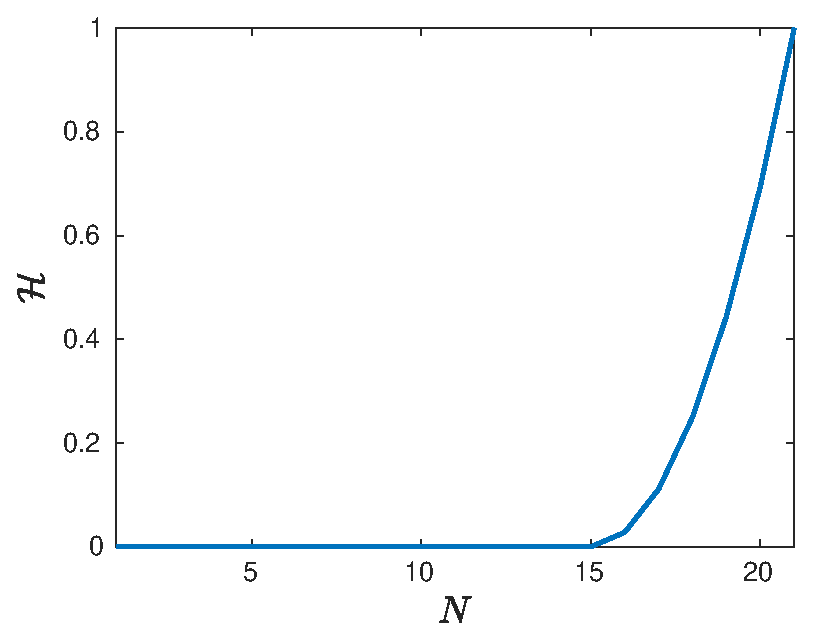
\includegraphics[width=0.60\textwidth]{filter_shape}
	\caption{Transfer function for the spectral coefficients for the filter $\mathcal{H}$ with number of modes $N=21$ and cut-off mode number $N_{c}=16$.}
	\label{fig:filter_shape}
\end{figure}

Several parameter optimization studies were performed to determine the optimum value of $\chi$ and filter shape $\mathcal{H}$ using turbulent channel flow simulations. The LES results were compared with the DNS database of \cite{moser99} and the optimum parameters were further validated for a flow around a wing section at $Re_{c}=400,000$. A good agreement was found between the LES and the DNS data of \cite{hosseini16}, and the optimized parameters were then used for all subsequent simulations.

\section{Arbitrary-Lagrangian-Eulerian (ALE)}

Typical solutions of unsteady fluid flows utilize the Eulerian framework where the coordinate system is fixed in space. A fixed coordinate system however becomes infeasible when the domain boundaries are in motion, as is the case of fluid-structure interaction problems, or when there is a free surface which may lead to a deforming interface. An appropriate method is needed to account or the motion of the boundaries and/or the interior grid points. One such method which substantially simplifies the difficulties arising out of moving boundaries is the Arbitrary-Lagrangian-Eulerian (ALE) method. The method was proposed in a finite-difference framework by \cite{hirt74} and later brought to the spectral-element framework by \cite{ho90,ho91}. The technique combines both the Lagrangian and Eulerian formulations such that, the Navier--Stokes may be solved with the grid points moving with the fluid elements \textit{i.e.} in a Lagrangian framework, or with fixed grid points (Eulerian), or with grid points moving in an arbitrary prescribed manner. The heart of the technique lies in the formulation of the total time rate of change of a quantity in the ALE frame, defined analogously to the material derivative. Thus for a quantity $\mathbf{F(x_{i},t)}$, the change due to small increments $dx_{i}$ and $dt$ may be expressed as \citep{kundu02}
\begin{align}
	dF = \frac{\partial F}{\partial t}dt + \frac{\partial F}{\partial x_{i}}dx_{i}.
	\label{eqn:material_deriv_df}
\end{align}
One may choose to follow any arbitrary path along which this quantity is evaluated, in which case the quantities $dx_{i}$ and $dt$ are related by the velocity of the (grid) point along this arbitrary path $w_{i} = dx_{i}/dt$. The relation results in the expression referred to as the ALE derivative \citep{deville02}, here denoted as $\delta F/\delta t$ to differentiate it from the very similar expression for the material derivative (which is evaluated along the fluid particle trajectory)
\begin{align}
\frac{\delta F}{\delta t} = \frac{\partial F}{\partial t} + w_{i}\frac{\partial F}{\partial x_{i}}.
\label{eqn:ale_derivative}
\end{align}
When $w_{i}$ is equal to the fluid velocity $u_{i}$, we recover the familiar Lagrangian expression for the material derivative $DF/Dt$. On the other hand, when $w_{i}=0$, we get the local (Eulerian) rate of change of the quantity $F$. The material derivative and the ALE derivative share a simple relationship defined using a relative velocity of the fluid particle with respect to the grid motion $c_{i} = u_{i} - w_{i}$, which may be used in the definition of material derivative to obtain
%\begin{subequations}
	\begin{align}
%	\frac{DF}{Dt} = \frac{\partial F}{\partial t} + u_{i}\frac{\partial F}{\partial x_{i}} \nonumber\\
%	\frac{DF}{Dt} = \bigg(\frac{\partial F}{\partial t} + w_{i}\frac{\partial F}{\partial x_{i}}\bigg) + c_{i}\frac{\partial F}{\partial x_{i}} \nonumber \\	
	\frac{DF}{Dt} = \frac{\delta F}{\delta t} + c_{i}\frac{\partial F}{\partial x_{i}}.
	\label{eqn:ale_material_derivative}
	\end{align}
%\end{subequations}
Thus the Navier--Stokes in the ALE formulation may be expressed as 
\begin{subequations}
	\label{eqn:ale_navier_stokes}	
	\begin{align}
	\frac{\delta u_{i}}{\delta t} + (u_{j} - w_{j})\frac{\partial u_{i}}{\partial x_{j}} =  - \frac{1}{\rho}\frac{\partial p}{\partial x_{i}} + \frac{1}{Re}\bigg(\frac{\partial^{2} u_{i}}{\partial x_{j}\partial x_{j}}  \bigg) +f_{i}, \\
	\frac{\partial u_{i}}{\partial x_{i}} = 0,
	\end{align}
\end{subequations}
where $w_{j}$ is the velocity of the grid points. The solution of the Navier--Stokes is then a simple matter of evaluating a suitable grid velocity. 

In many cases, such as the flow over an oscillating airfoil, the velocity of the grid points at the boundary (airfoil surface) may be explicitly known. \cite{ho90,ho91} propose to extend this velocity to the interior points of the domain by solving an elliptic problem for the mesh velocity. In the present work we take a simpler approach to prescribing the mesh velocities in the interior domain. Recognizing the simple trigonometric form of a harmonic pitching motion, all mesh points may simply be prescribed a solid body rotation with the instantaneous angular velocity of the airfoil. However a pure solid-body rotation would also displace the domain boundaries. Therefore a damping function is used to smoothly reduce the rotational velocity away from the airfoil boundary such that the mesh motion is zero at the far-field, inlet and outflow boundaries. Thus for an airfoil with an instantaneous rotation rate of $\Omega_{z}(t)$, the mesh velocity is prescribed as:
\begin{align}
	w_{i}(x,y,z,t) = \underbrace{(\Omega_{z}(t) \times \vec{R})}_{\text{Solid body rotation}} \overbrace{f(|\ \vec{r}\ |)}^{Damping}
	\label{eqn:mesh_velocity}
\end{align}
where $\vec{r}$ is the normal distance of a grid point from the airfoil surface, $\vec{R}$ is the distance from the rotational axis and $f(r)$ is a damping function which can be prescribed in many different ways, depending on one's preferences. The damping function needs to have two essential properties, \textit{i.e.} it must be equal to 1 when $|\vec{r}|=0$, which implies the mesh points at the airfoil boundary move with the surface (solid body rotation at the airfoil surface), and it must smoothly decay to zero close to the far-field boundaries, which allows the external boundaries of the computational domain to remain fixed in physical space. Figure~\ref{fig:mesh_rotation_damping} shows the damping function used in the present work as a function of the normal distance from the airfoil surface.
\begin{figure}[h]
	\centering
	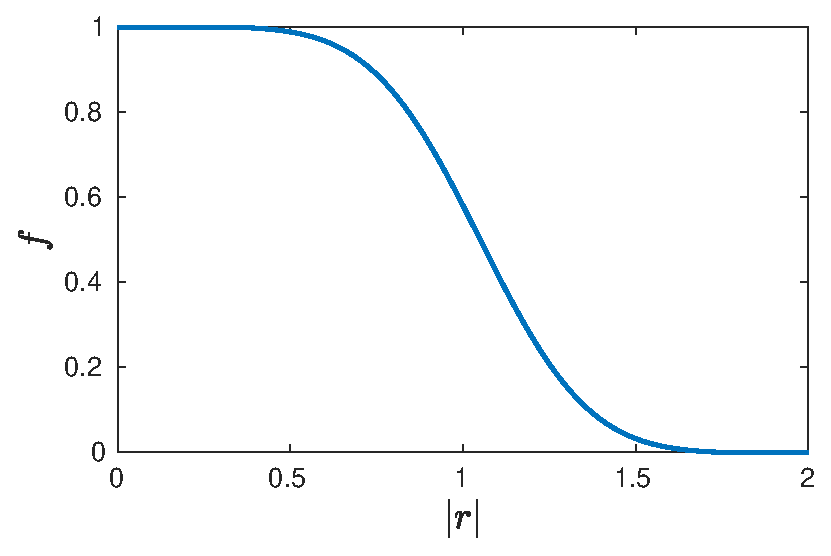
\includegraphics[width=0.55\textwidth]{damping_func}
	\vspace{5pt}
	\caption{Damping function $f(r)$ for the mesh velocities.}
	\label{fig:mesh_rotation_damping}
\end{figure}
The damping function moves the grid points close to the airfoil surface with the same rotational velocity of the airfoil and spreads out the mesh deformation into the interior of the domain. This damping function is calculated once at the beginning of the simulation. Hence all quantities $\Omega_{z}(t),\ \vec{r},\ f(r)$ which are needed for prescribing the mesh velocity are explicitly known at each time-step without the need for solving an elliptic equation as in \cite{ho90,ho91}. 

\section{Free-stream turbulence}

Isotropic, homogeneous free-stream turbulence is prescribed at the inlet and far-field boundaries to add small disturbances to the flow-field, which simulate the disturbances found in a wind-tunnel or in free-flight conditions. The free-stream turbulence is prescribed as a superposition of Fourier modes with a random phase shift. The maximum and minimum amplitudes of the wavenumber vector are prescribed quantities and are limited by the resolution of the spatial discretization and size of the domain respectively. The wavenumber space between the minimum and the maximum is divided into 20 concentric shells with each shell representing the amplitude of the three-dimensional wavenumber vectors lying on the shell. 20 points are randomly chosen on each shell with the location of each point representing the three-dimensional components of the wavenumber vector. Thus the free-stream turbulence is represented by a total of 400 fourier modes. Care is taken to avoid very small wavenumber components which result in wavelengths in physical space that are larger than the computational domain. The streamwise length scales are transformed to a temporal frequency by invoking Taylor's frozen turbulence hypothesis and using the local mean streamwise velocity at the inlet for the space-time conversion. The amplitude of the free-stream modes on each spherical shell is scaled using the von K\'arm\'an spectrum. Figure~\ref{fig:fst_duct} shows an instantaneous visualization of the streamwise velocities in a doubly-periodic duct flow case with high ($5\%$) free-stream turbulence intensity prescribed at the the inlet. Figure~\ref{fig:ti_decay} shows the spatial decay of turbulence intensity. After a small initial distance of adjustment from the inlet, the turbulence intensity decays as a power law. A very similar method for generating free-stream turbulence for simulations of flat-plate boundary layers is used by \cite{schlatterdiploma,brandt04,schlatter08} and more recently for wind turbine simulations by \cite{kleusberglicenciate}.

\begin{figure}[h]
	\centering
	\begin{subfigure}[t]{0.49\textwidth}
		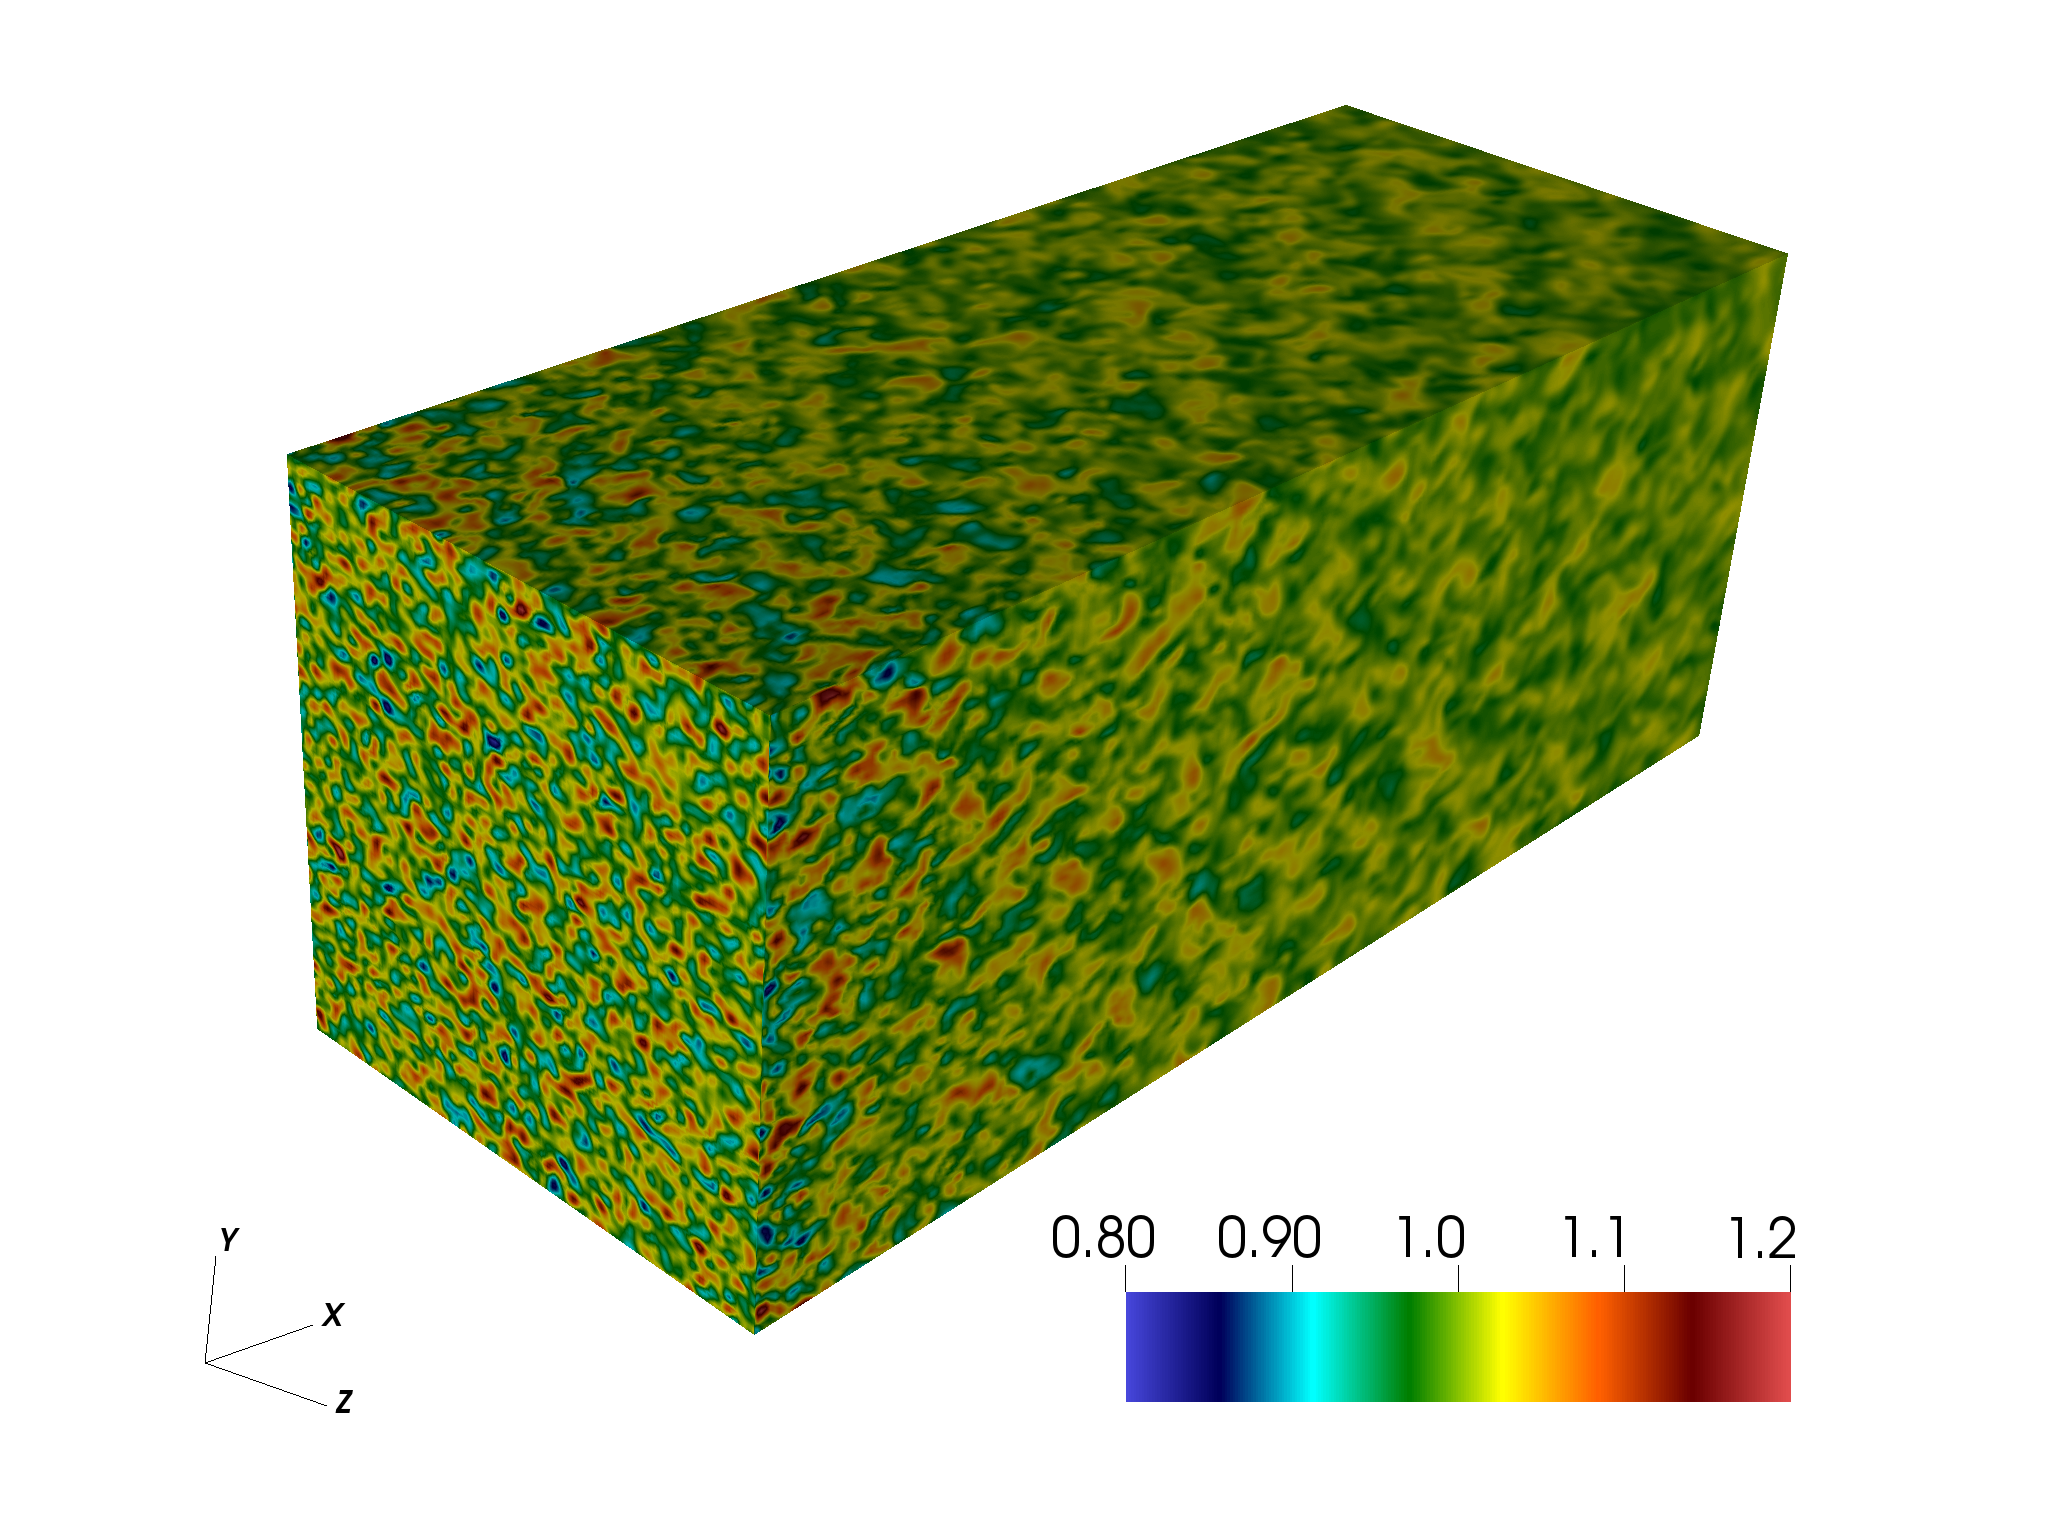
\includegraphics[width=1\textwidth]{fst_duct_vx0000.png}
		\caption{Visualization of free-stream turbulence prescribed at the inlet for a doubly periodic duct flow. Colors represent the instantaneous streamwise velocity.}
		\label{fig:fst_duct}
	\end{subfigure}
	\begin{subfigure}[t]{0.49\textwidth}
		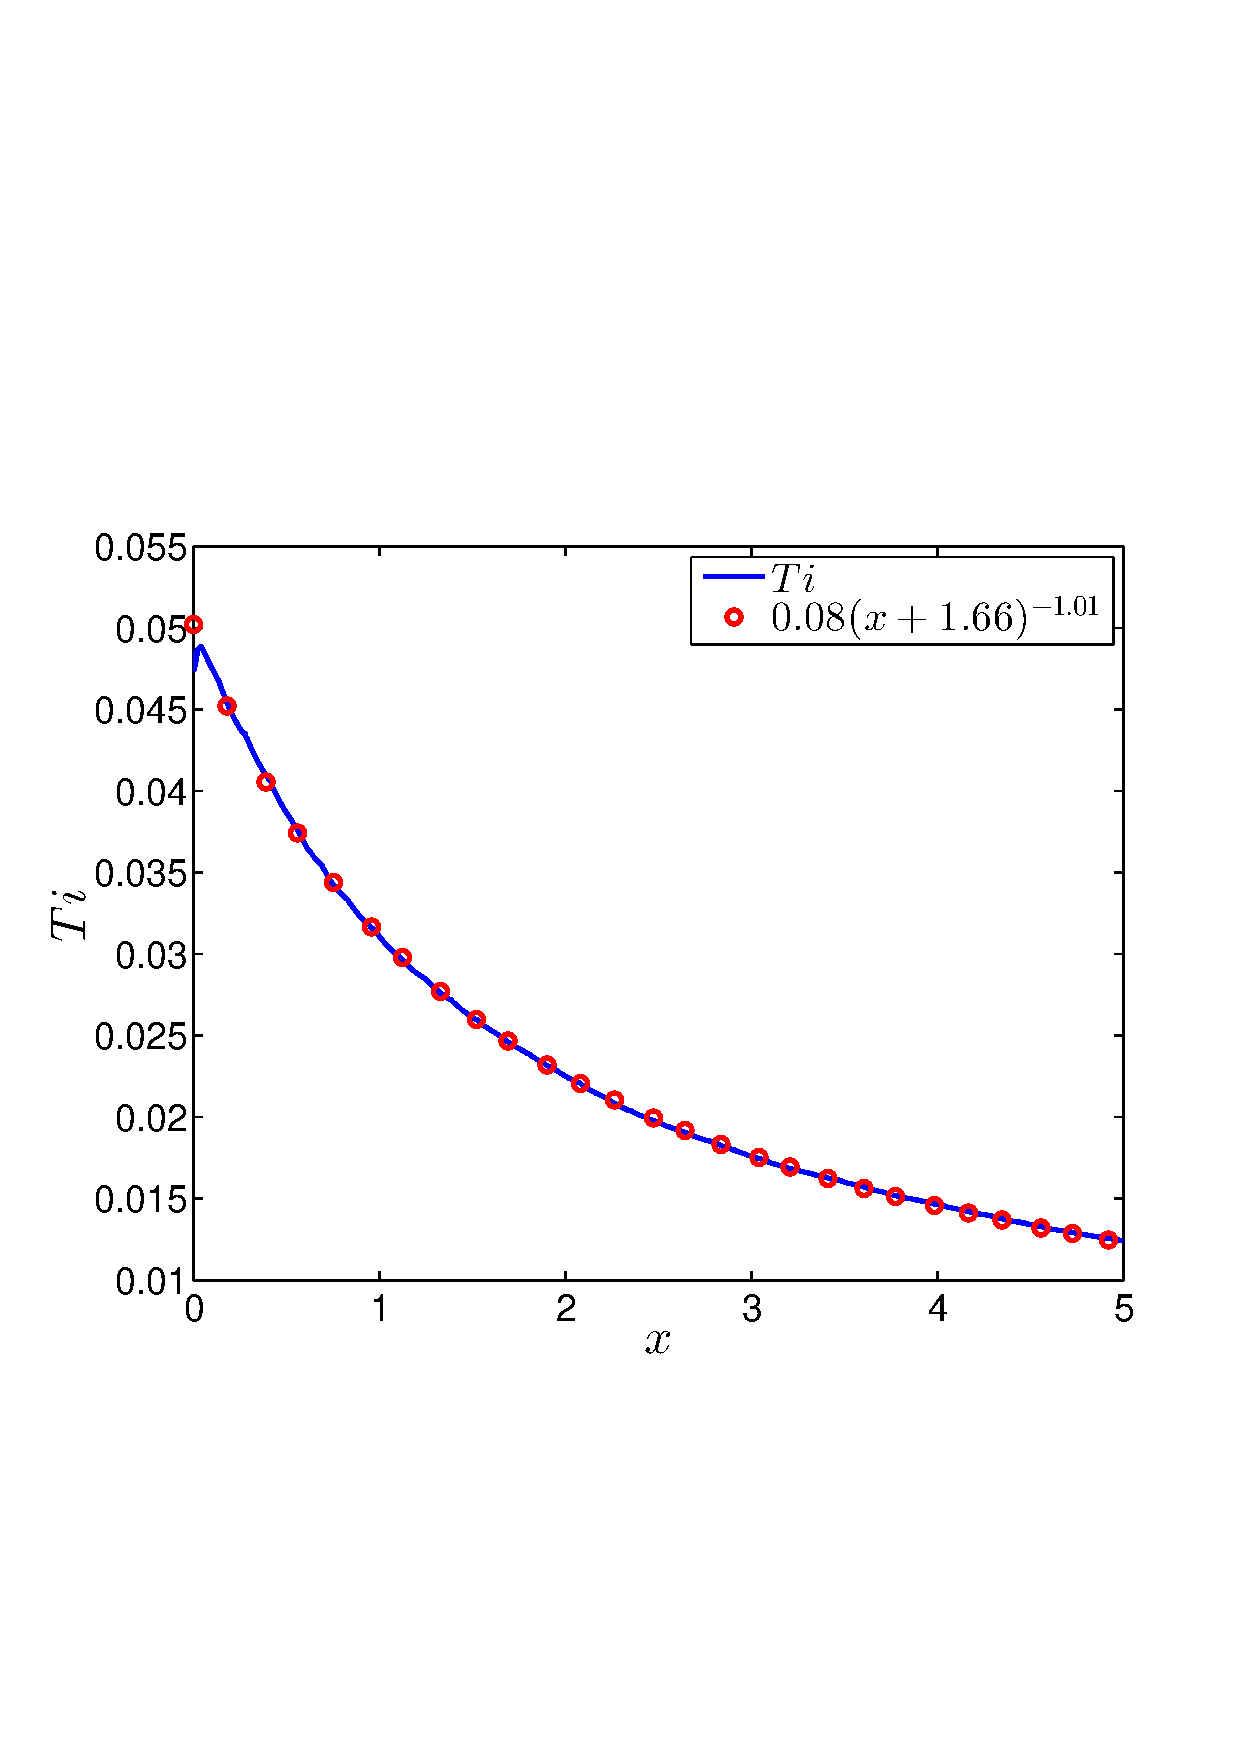
\includegraphics[width=1\textwidth]{ti_decay}
		\caption{Decay of turbulence intensity with streamwise distance, along with the least-squares fit of a power law.}
		\label{fig:ti_decay}
	\end{subfigure}
\end{figure}

%===============================================================================
\chapter{Overview of numerical simulations}
%===============================================================================

\section{Flow around unsteady wings}

The unsteady experiments of \cite{mai11,hebler13} and \cite{lokattthesis} have shown that aerodynamic non-linearities are related to the movement of transition over the suction side of the airfoil. Thus unsteady boundary layer dynamics play an important role in aerodynamic response of NLF airfoils. The present work investigates the unsteady boundary layers with a particular focus on unsteady transition with the aim to shed light on the phenomenon of non-linear unsteady aerodynamic response. The airfoil used in the investigation is the ED36F128 (with a $13.8^{\circ}$ flap deflection), designed at the Aeronautical and Vehicle Engineering department at KTH. It is a natural laminar flow airfoil, which has been used in several steady and unsteady experiments \citep{lokatt17,lokattthesis}. The unsteady experiments have shown the non-linearities that appear to be typical of laminar airfoils \citep{lokattthesis}. The results of the steady and unsteady experiments using this airfoil have been made available to us by Dr. Eller and Dr. Lokatt. Non-linearities in the unsteady aerodynamic forces are observed for only a certain range of angle of attack $\alpha$. Therefore a careful assessment of the data was needed in order to select the right parameter range where the relevant flow physics could be observed in the numerical simulations. The data in the experimental campaign was gathered primarily through pressure taps located around airfoil for the calculation of unsteady aerodynamic forces. Thus measurements of the unsteady boundary layer characteristics was not available through the experimental data. Calculations using an integral boundary layer code XFOIL \citep{drela89}, were used to complement the experimental data and better evaluate the state of the boundary layer in the static measurements.

Figure~\ref{fig:tr_xfoil_100_750} shows the calculated transition locations for two different Reynolds numbers ($Re_{c}=100,000$ and $Re_{c}=750,000$) using XFOIL and figure~\ref{fig:765k_static_cz_foil} shows the experimentally measured normal force coefficient as well as calculations from XFOIL for $Re_{c}=750,000$. For the higher Reynolds number case, transition location varies sharply with angle of attack within the range $3.4^{\circ}<\alpha<6.5^{\circ}$. Aerodynamic non-linearities can also be observed approximately within the same angle of attack range (figure~\ref{fig:765k_static_cz_foil}). For the lower Reynolds number case, no experimental data is available. Therefore solely XFOIL calculations are used and the parameter range is selected where the transition location varies rapidly with angle of attack. This is found for an angle of attack range of $6.7^{\circ}<\alpha<8.0^{\circ}$.
\begin{figure}[!h]
	\centering
	\begin{subfigure}[t]{0.45\textwidth}
		\caption{}
		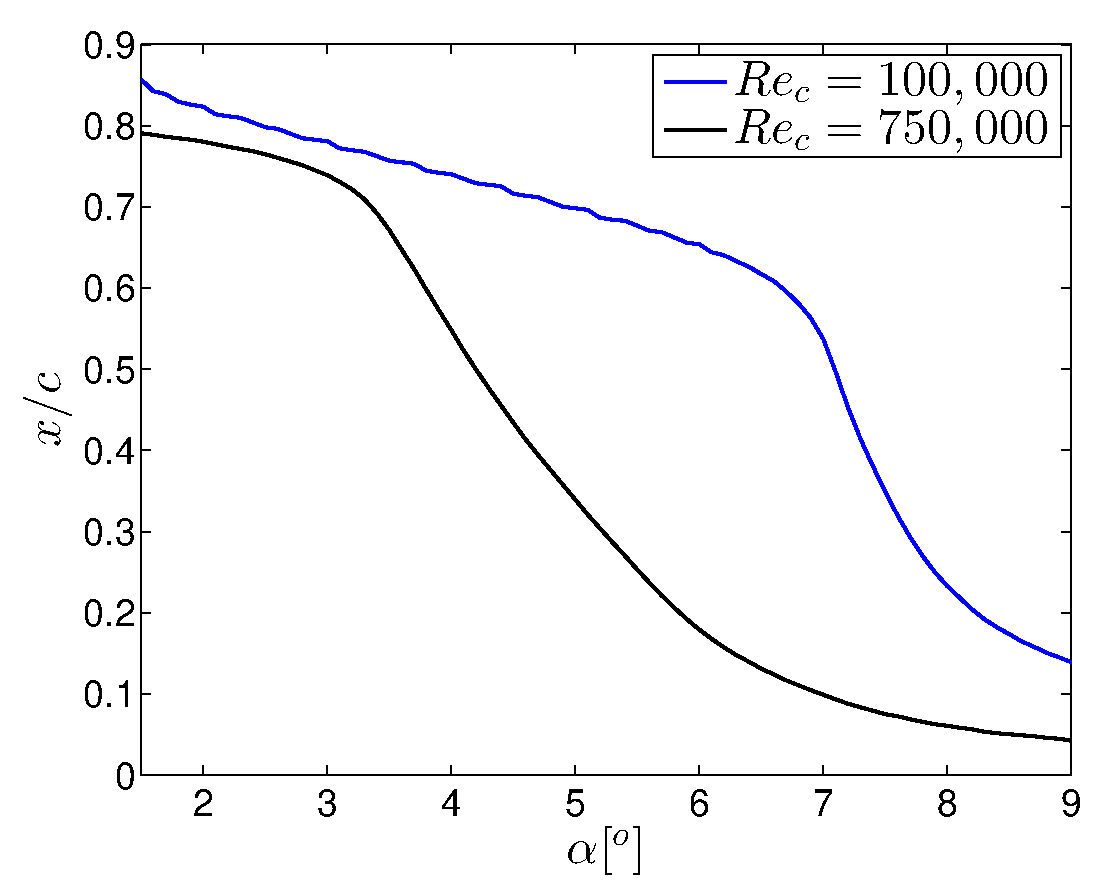
\includegraphics[width=1\textwidth]{tr_xfoil_100_750}
		\label{fig:tr_xfoil_100_750}		
	\end{subfigure}
	\begin{subfigure}[t]{0.45\textwidth}
		\caption{}
		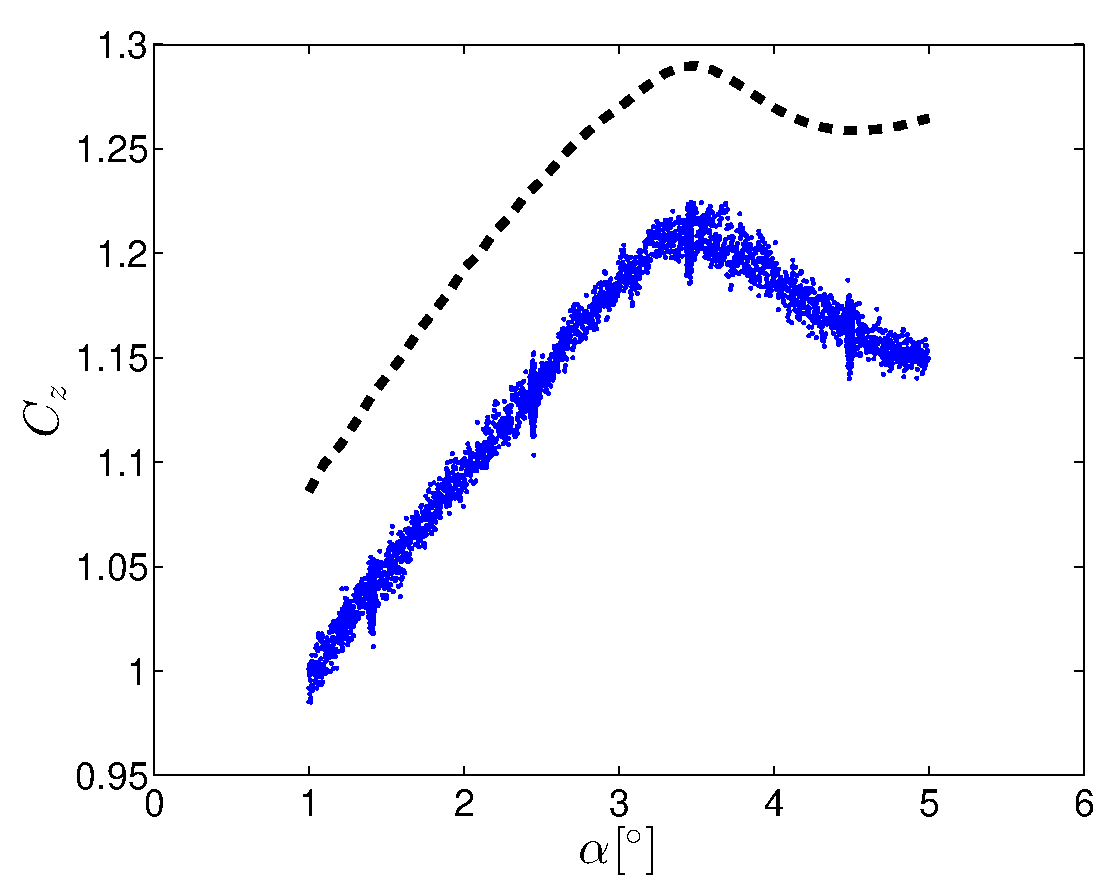
\includegraphics[width=1\textwidth]{765k_static_model_cz_xfoil}
		\label{fig:765k_static_cz_foil}
	\end{subfigure}
	\caption{(a) Transition location calculated using XFOIL for two different Reynolds numbers. (b) Normal force coefficient measured in experiments (dots) and from XFOIL calculations (dashed line) for $Re_{c}=750,000$.}		
\end{figure}
Numerical simulations are performed with stationary airfoils to ensure the expected static boundary layer characteristics are captured by the numerical simulations.  Figure~\ref{fig:overview_la2_750k_stationary} depicts the instantaneous vortical structures in the flow for $Re_{c}=750,000$ for an angle of attack $\alpha=2.4^{\circ}$ and $\alpha=4.4^{\circ}$ which shows the change in boundary layer characteristics in the static cases. Similarly, figure~\ref{fig:overview_isocontour_aoa} shows the static boundary layer characteristics for $Re_{c}=100,000$ at $\alpha=6.7^{\circ}$ and $\alpha=8.0^{\circ}$.
\begin{figure}[h]
	\centering
	\begin{subfigure}[t]{0.49\textwidth}
		\caption{$\alpha=2.4^{\circ}$}		
		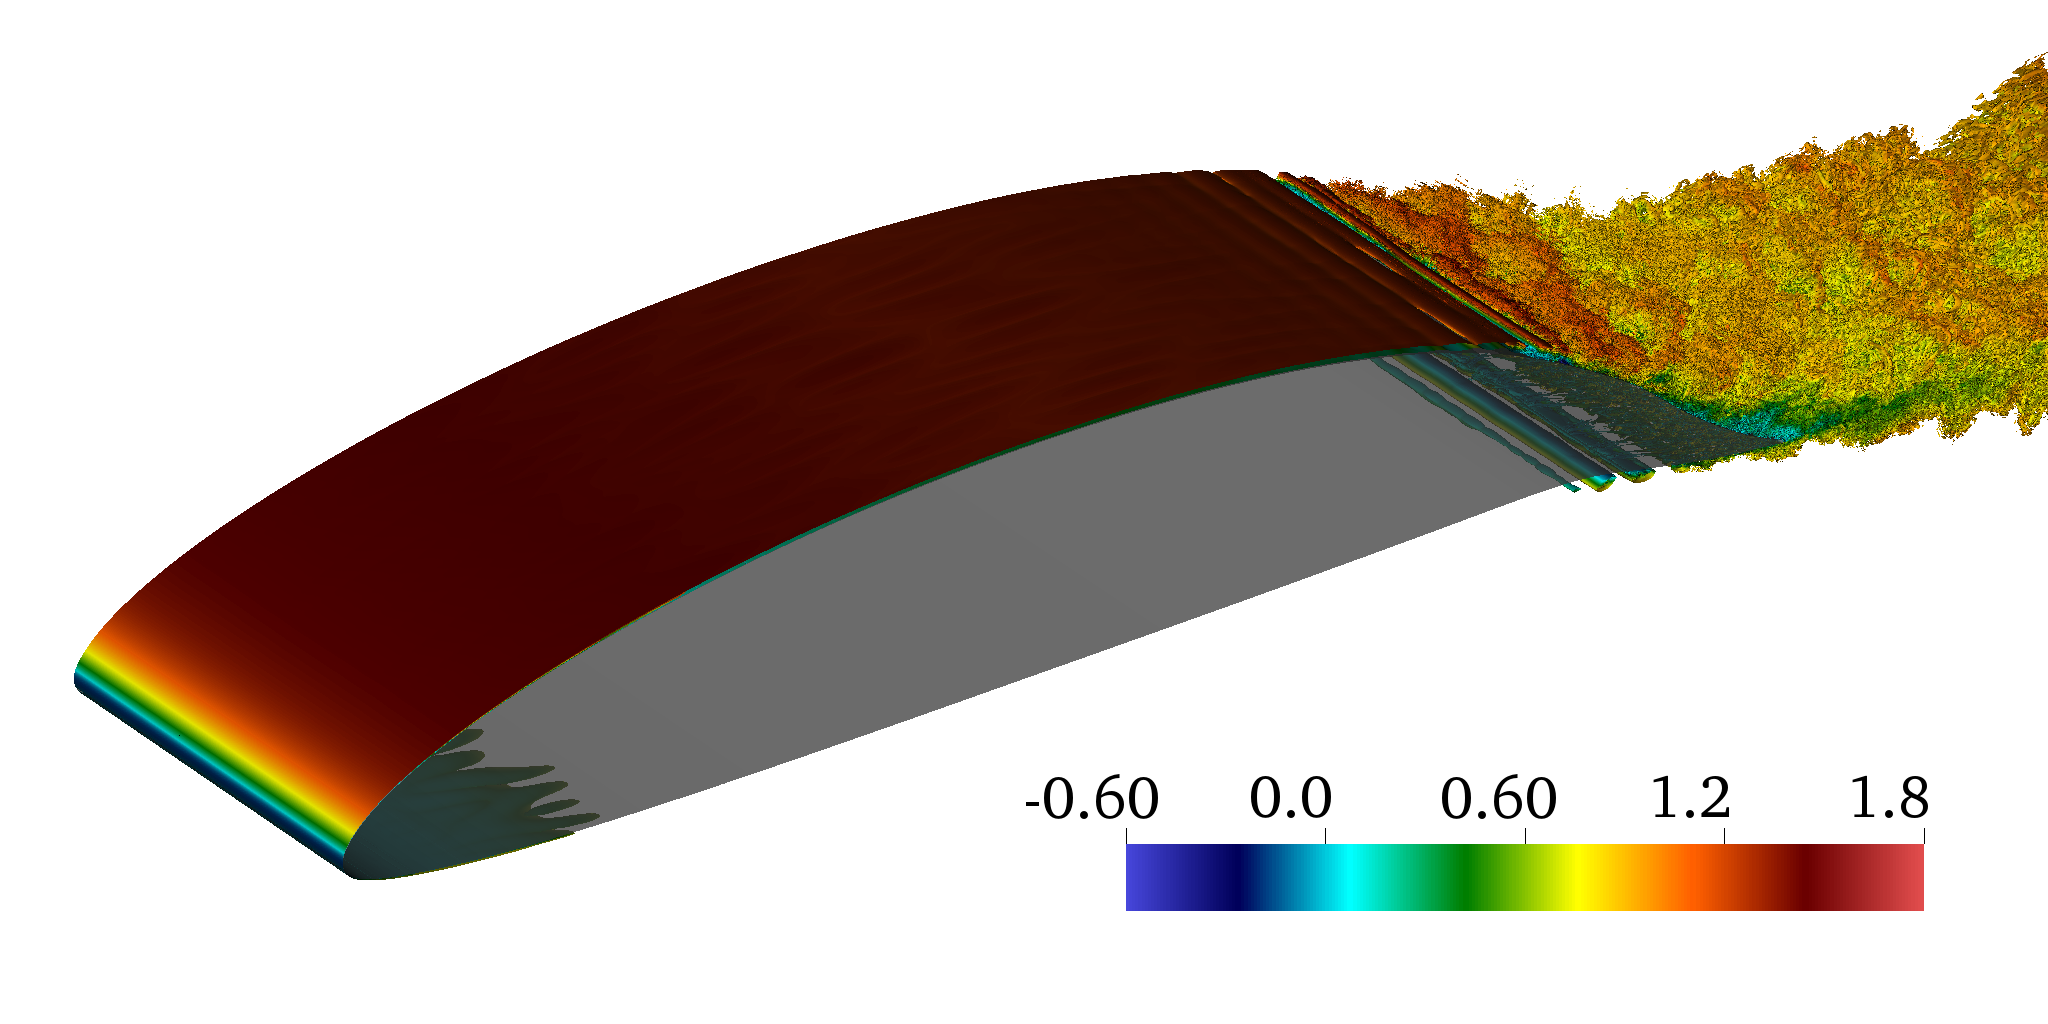
\includegraphics[width=1\textwidth]{paper2/imgs2/pitch_re750k0001}
		\label{fig:overview_la2_aoa24}
	\end{subfigure}
	\begin{subfigure}[t]{0.49\textwidth}
		\caption{$\alpha=4.4^{\circ}$}		
		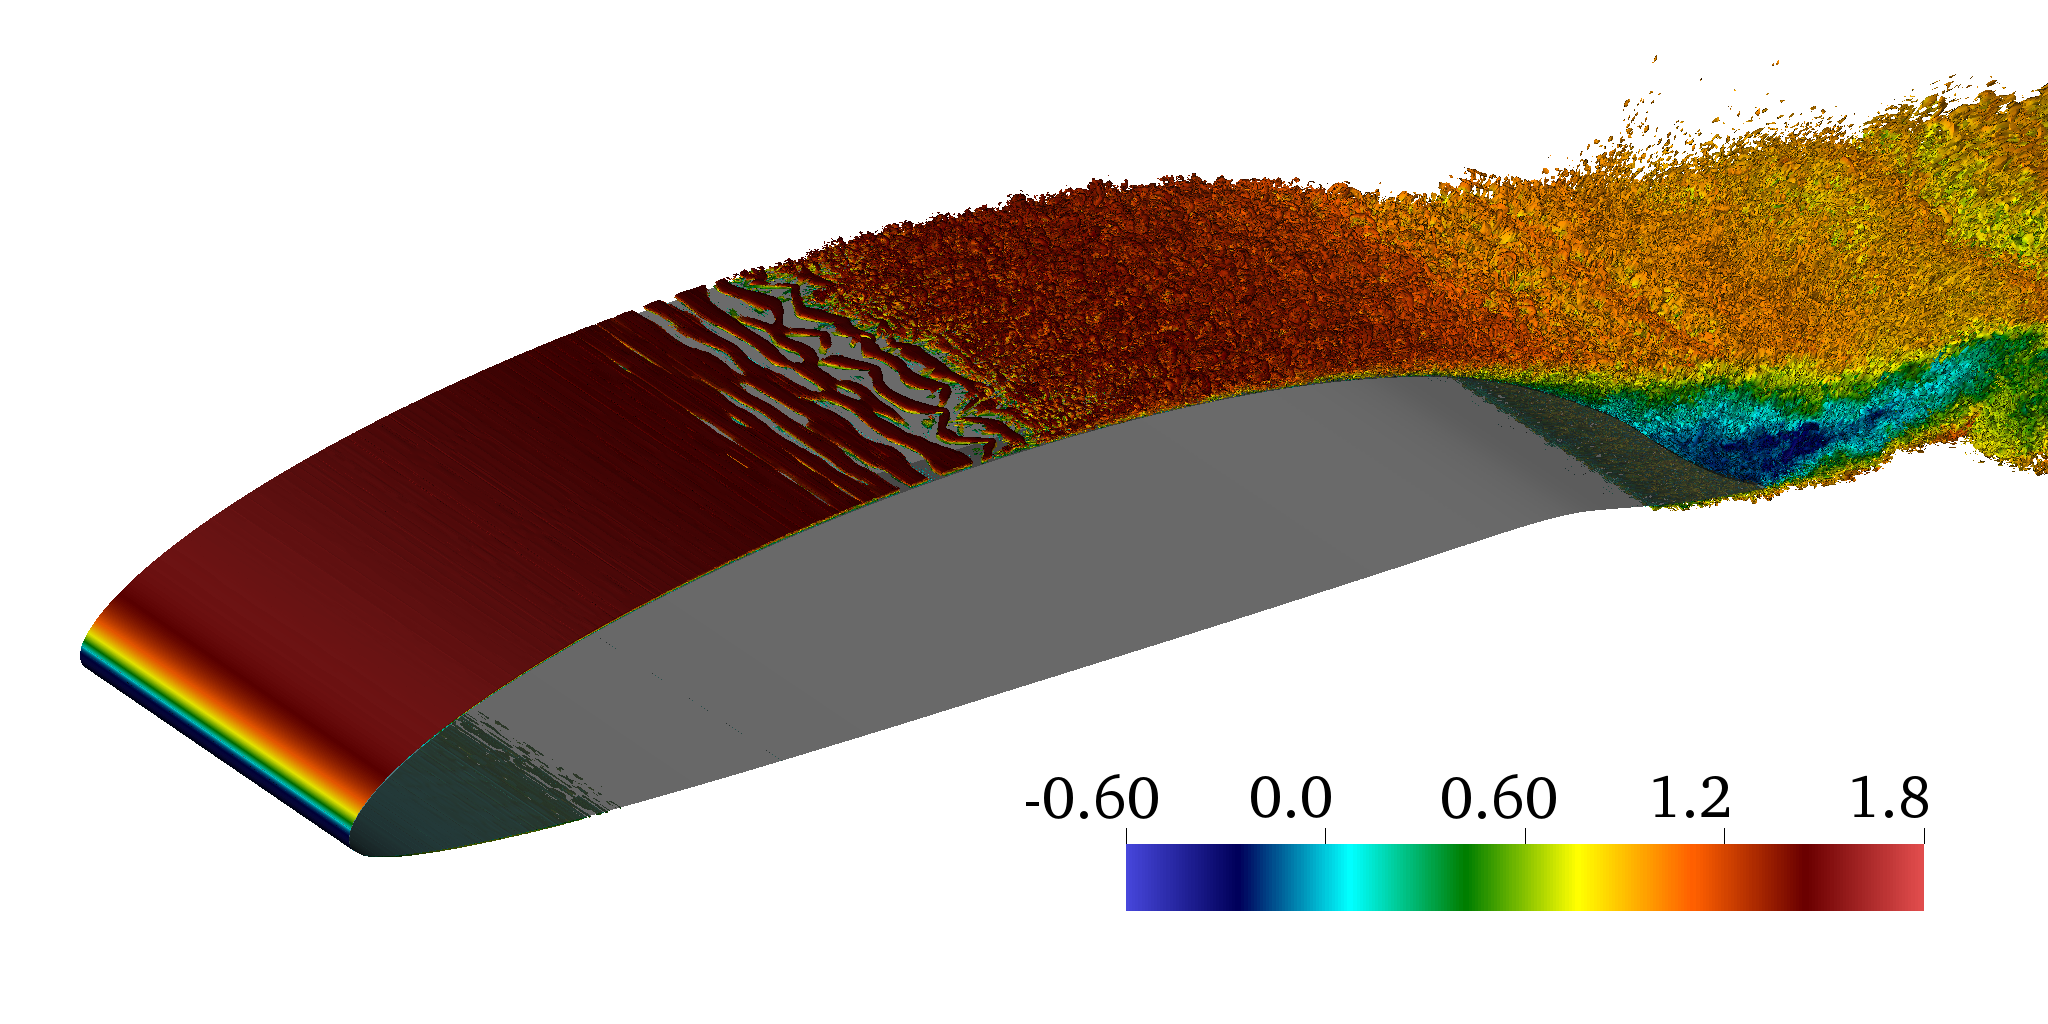
\includegraphics[width=1\textwidth]{paper2/imgs2/pitch_re750k0002}
		\label{fig:overview_la2_aoa44}		
	\end{subfigure}	
	\caption{Instantaneous vortical structures identified by the $\lambda_{2}$ criterion for the two stationary angle of attack simulations at $Re_{c}=750,000$.}
	\label{fig:overview_la2_750k_stationary}
\end{figure}

\begin{figure}[t]
	\begin{subfigure}[b]{0.49\textwidth}
		\centering
		\caption{$\alpha=6.7^{\circ}$}		
		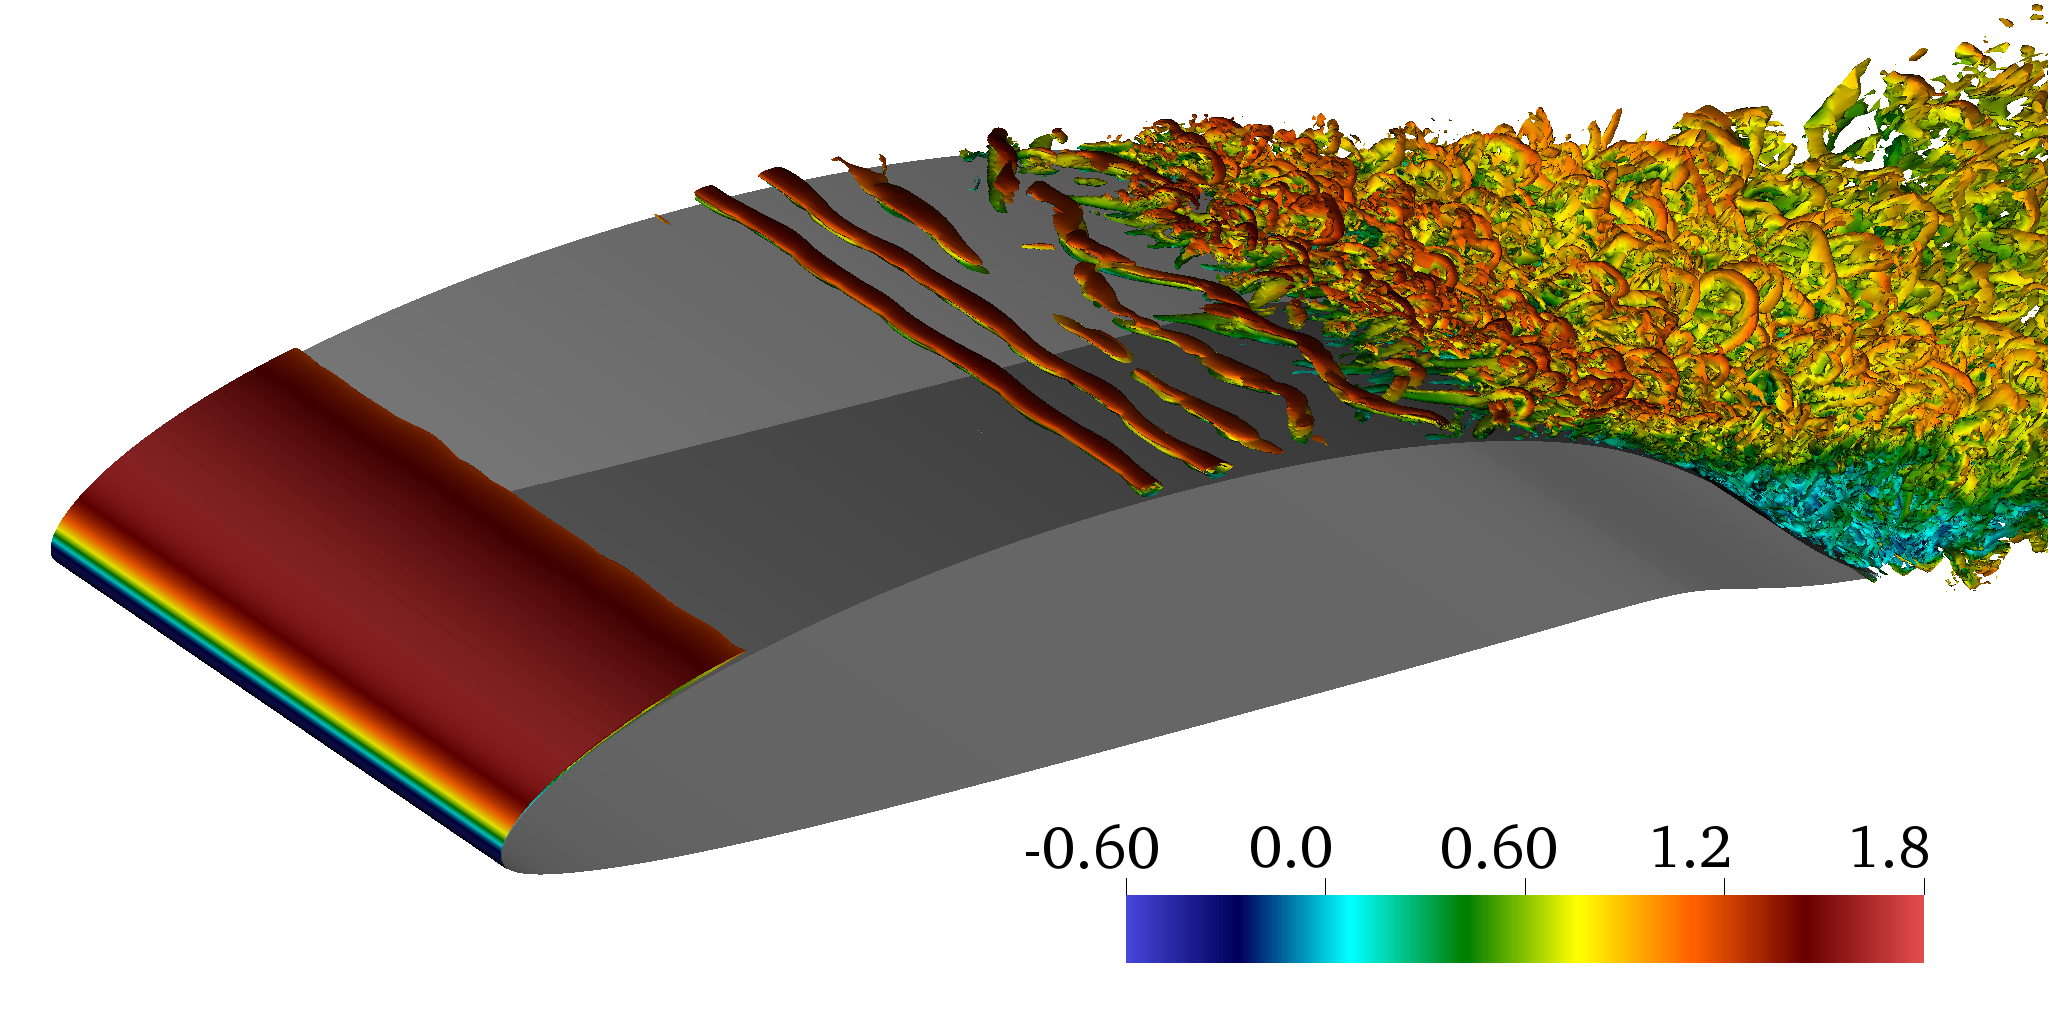
\includegraphics[width=1\textwidth]{paper3/imgs/re100k_static67_0001}
		\label{fig:overview_aoa67_iso}
	\end{subfigure}
	\begin{subfigure}[b]{0.49\textwidth}
		\centering
		\caption{$\alpha=8.0^{\circ}$}		
		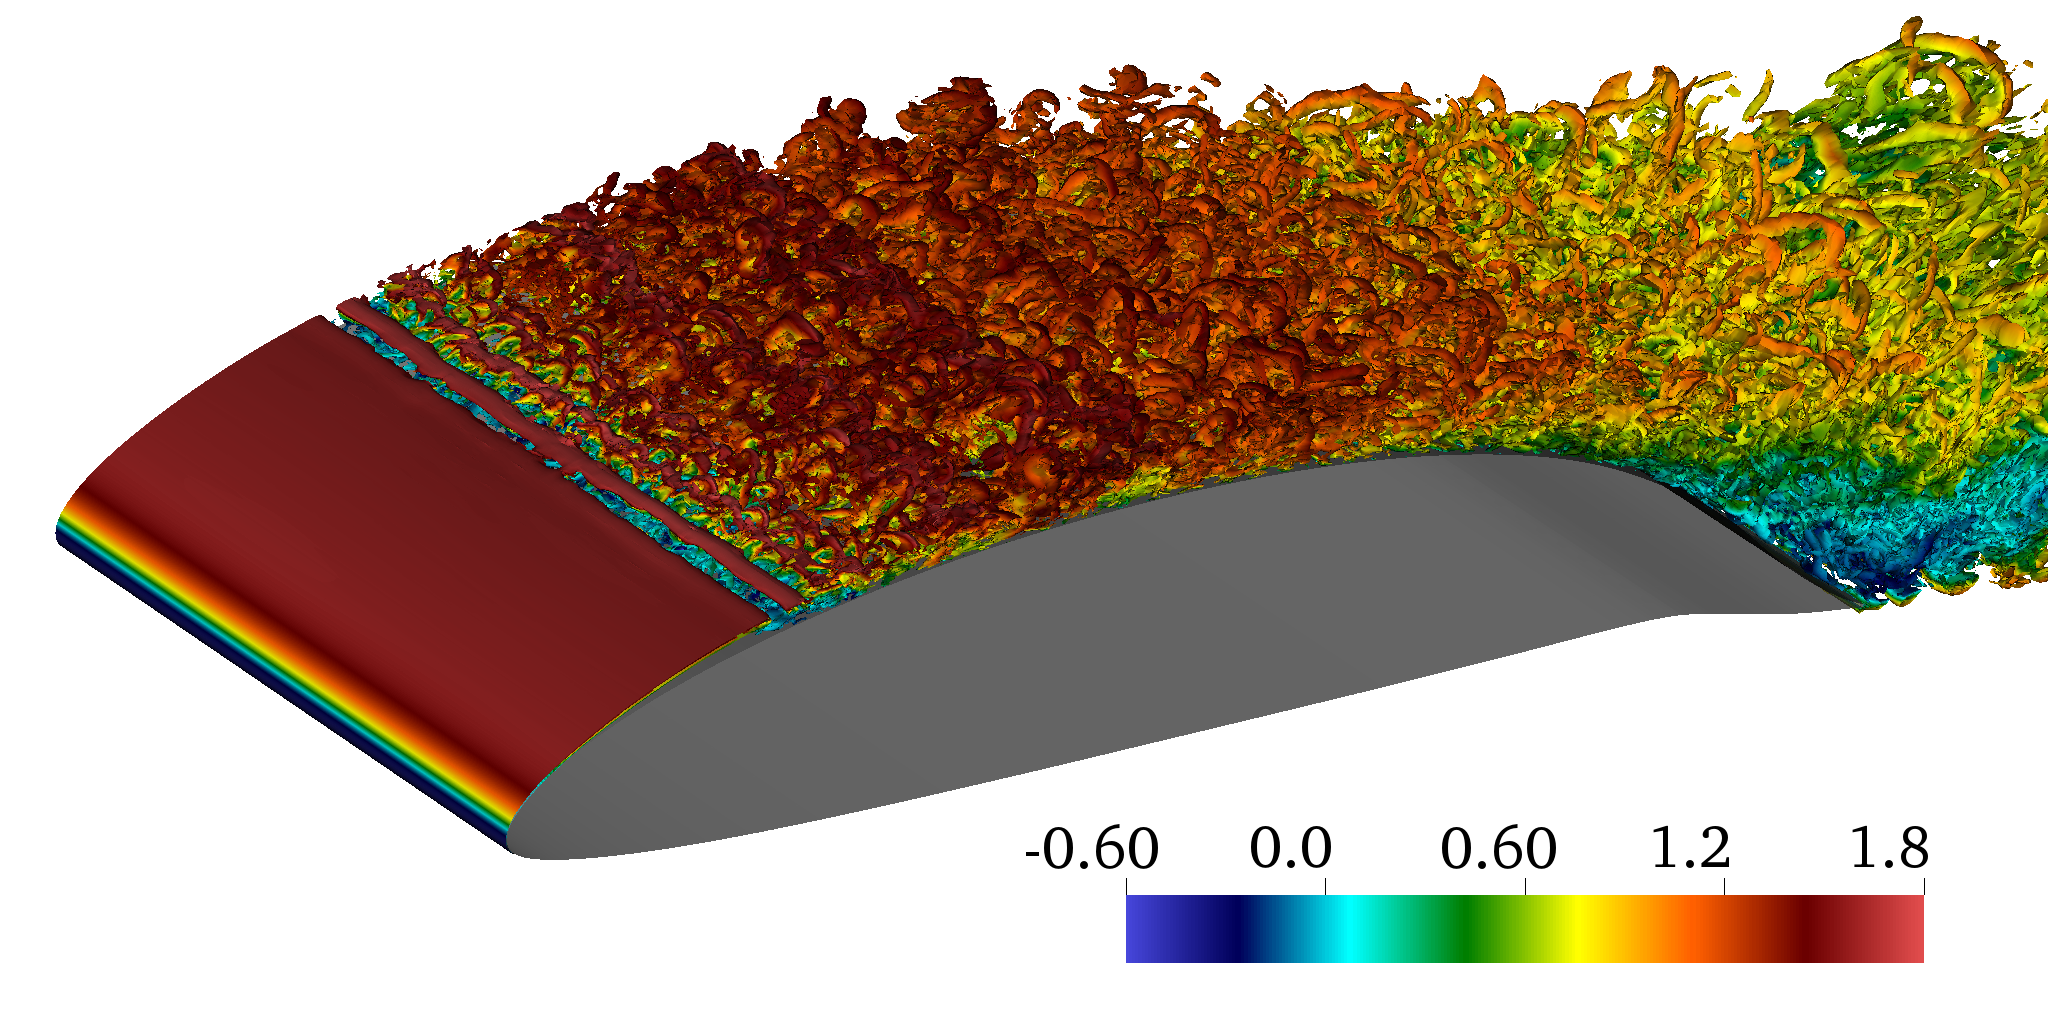
\includegraphics[width=1\textwidth]{paper3/imgs/re100k_static80_0001}
		\label{fig:overview_aoa80_iso}
	\end{subfigure}
	\caption{Isocontours of instantaneous $\lambda_{2}$ structures observed for two different (stationary) angles of attack at $Re_{c}=100,000$.}
	\label{fig:overview_isocontour_aoa}
\end{figure}

For both the Reynolds number cases, significant temporal variation of transition location is also found for the unsteady cases. Figure~\ref{fig:overview_transition_alpha} shows the variation of transition with respect to $\alpha$. The transition locations were calculated using thresholds on the instantaneous spanwise-averaged Reynolds stress $\overline{u'v'}$ and spanwise fluctuation intensity $\overline{w'w'}$. For the lower Reynolds number case the boundary layer also develops a leading-edge laminar separation bubble during the pitch cycle which significantly influences the boundary-layer dynamics.

\begin{figure}[t]
	\begin{subfigure}[b]{0.49\textwidth}
		\centering		
		\includegraphics[width=1\textwidth,height=0.80\textwidth]{imgs/750k_transition_alpha.eps}
	\end{subfigure}
	\begin{subfigure}[b]{0.49\textwidth}
		\centering	
		\includegraphics[width=1\textwidth]{paper3/imgs/transition_alpha.eps}
	\end{subfigure}
	\caption{Phase portraits of transition location for (left) $Re_{c}=750,000$ and (right) $Re_{c}=100,000$.}
	\label{fig:overview_transition_alpha}
\end{figure}


\section{Flow around a stationary wing section}

The final paper in the thesis deals with the study of the boundary layer over a wing section at a chord-based Reynolds number of $Re_{c}=1,000,000$. The airfoil used for the study is the asymmetric NACA 4412. A DNS database for the flow around the same airfoil at $Re_{c}=400,000$ is available and comparisons are made between the two cases to assess the effects of changing Reynolds number on the developing boundary layer. The numerical setup is done in a manner very similar to the computational study by \cite{hosseini16}. Figure~\ref{fig:overview_flow_field_re1000k} shows a section of the numerical grid and the instantaneous vortical structures in the flow field. Figure~\ref{fig:overview_beta_Reth_Ret} shows a comparison of the different measures of the boundary layer over the chord-wise distance for the two different Reynolds numbers. While both wall-shear stress (indicated by $Re_{\tau}$) and boundary layer thickness (measured with momentum thickness Reynolds number $Re_{\theta}$) change between the two cases, the Clauser parameter stays nearly the same throughout the chord. This allows comparisons across different Renolds numbers without ambiguity since the pressure gradient histories remain the same with changing Reynolds numbers. 
\begin{figure}[t]
	\centering
	\includegraphics[width=0.49\textwidth]{paper4/imgs/wing_mesh}
	\includegraphics[width=0.49\textwidth]{paper4/imgs/wing_visualization}
	\caption{(Left) Two-dimensional slice of the computational domain showing the spectral-element distribution. (Right) Instantaneous flow field showing coherent structures identified with the $\lambda_{2}$ method \citep{jeong95}, and colored with horizontal velocity. In this figure, dark blue represents a horizontal velocity of $-0.1$ and dark red a value of $2$.}
	\label{fig:overview_flow_field_re1000k}
\end{figure}

\begin{figure}[t]
	\centering
	\includegraphics[width=0.49\textwidth]{paper4/imgs/beta_vs_x}
	\includegraphics[width=0.49\textwidth]{paper4/imgs/Reth_vs_x}
	\includegraphics[width=0.49\textwidth]{paper4/imgs/Ret_vs_x}
	\caption{Streamwise evolution of (top left) the Clauser pressure-gradient parameter $\beta$, (top right) the Reynolds number based on momentum thickness $Re_{\theta}$ and (bottom) the friction Reynolds number $Re_{\tau}$, for the two wing cases under study.}
	\label{fig:overview_beta_Reth_Ret}
\end{figure}

%===============================================================================
\chapter{Conclusions and outlook}
%===============================================================================

The current thesis work concerns three different fields of research.

In the first part of the thesis, the ``evolve and filter'' technique for the stabilization of spectral-element methods is analyzed and it is found the filter operation causes an undesirable loss of divergence-free quality of the solution. This loss of divergence is shown to be particularly large for the test case of a double shear layer. An alternate formulation of the stabilization called the relaxation-term (RT) stabilization is shown to overcome the drawbacks of the explicit filtering technique, while maintaining the simplicity of the original explicit filter. This RT stabilization technique is very closely related to explicit filtering, with the two operations being equivalent to the leading order in time. Stability limits of the RT stabilization are explored and is shown to be stable within the practical parameter range.

In the second part, an NLF airfoil undergoing small-amplitude pitch-oscillations is analyzed at two different Reynolds numbers. In both cases a large variation of transition, and thus boundary layer characteristics is observed over the airfoil resulting in a non-linear response of the aerodynamic force coefficients. For $Re_{c}=750,000$ it shown that the temporal evolution of the transition point can be understood with a simple phase-lag concept, with the implication that boundary-layer evolution may be considered quasi-steady in time. Using this phase-lag concept a simple empirical model is developed which is able to explain a fairly wide range of experimental data.

On the other hand, for $Re_{c}=100,000$ a qualitatively different picture emerges for the unsteady boundary layer. The boundary-layer response displays a dynamically rich behavior with marked asymmetry of upstream and downstream transition movement. In this case, transition location is governed by the properties of the leading-edge laminar separation bubble (LSB) and it is conjectured that the absolute instability of the LSB may be responsible for abrupt changes in boundary layer characteristics.

Finally, in the third part of the study, flow over a stationary NACA 4412 airfoil is studied at two different Reynolds numbers with the aim of better understanding the boundary-layer evolution in non-equilibrium pressure gradient boundary layers. Two flow cases at a chord-based Reynolds number of $Re_{c}=400,000$ and $Re_{c}=1,000,000$ are compared at different streamwise locations. It is found that the effect of the streamwise pressure gradients is higher at low Reynolds numbers, leading to greater energy in the larger structures present in the outer part of the turbulent boundary layer.

The current work has laid the foundation for several interesting questions that may be the focus of future work. Can the simple empirical aerodynamic model be extended for a wider range of unsteady motions? Can the phase-lag be predicted a-priori as in the case of the classical model by \cite{theodorsen35}? When does the quasi-steady assumption break down and the boundary layer becomes truly unsteady? For $Re_{c}=100,000$, can the asymmetry of the (upstream and downstream) velocities of transition point be linked with the stability properties of the LSB? What is the influence of free-stream turbulence on unsteady LSB? In stationary airfoils, how does the velocity spectrum change with Reynolds number in non-equilibrium flows? What are the characteristics of boundary layer streaks in non-equilibrium flows? Some of these questions will be the focus of further research.


%===============================================================================
% Acknowledgments
%===============================================================================
%


\begin{acknowledgements}
	My foremost gratitude goes to my supervisor Dan Henningson for giving me the opportunity to join his research group. His knowledge and guidance have helped me immensely as a student. His encouragement, for which there is no substitute, have always provided the inspiration I needed to constantly push myself further in my work. Next I would like to thank my co-advisors Philipp Schlatter and Ardeshir Hanifi. Philipp for his patience during all my ignorant and sometimes foolish questions on numerics, conferences, papers and others that I probably can't recall. Ardeshir for the laughter, the sandwiches, the beers and most importantly, always being available on short notice when I needed help. I would also like to thank the members of the NFFP project, Roger Larsson, Dr. David Eller and Dr. Mikaela Lokatt for all the interesting discussions on aerodynamics. 
	
	I am grateful to Adam Peplinski for all the help he provided with Nek5000, MPI and coding in general. I can not imagine figuring out the workings of Nek5000 without his support. Armin and Ricardo have helped me more than others during my crucial time as a new Phd student. The help is greatly appreciated.
	
	Special mentions go to Mattias for all the coffee breaks, introducing me to Swedish food, the spontaneous discussions and being the bouncing board for all my (mostly wrong) ideas. Your company shall be missed once you leave the department. Jacopo and Giandomenico for all the great company, joining for the spontaneous plans and granting me the honorary Italian citizenship. I'll learn Italian very soon I promise! Marco for the constant dinner company. Freddy for the weekend food+beer+movie routine. Elektra for being one of the greatest friends of all time. Politics, late-night and of course Trump shall keep us entertained for times to come. But mostly, thanks for correcting my manuscripts and the support during this licentiate period. A mention must also go to my unrequited love, Walter Fornari. Where will I find another like you?
	
	A hearty thanks goes out to all my friends here at the department who make this a wonderful place. Eric, Clio, Nicolas, Sudhakar, Ugis, Evelyn, Anthony, Mehdi, Ali, Guillaume, Luca, Luca, Pierluigi, enrico, Francesco, Kristina, Ekatrina, J.C., Matthias, Priti, Ninge, Sagar, Krishne, Dhiya, and everyone else. All of you, with your quirks, jokes, stories and gossip (looking at you Pierluigi) add a little bit of color to life everyday.
	
	Perhaps most importantly, my deepest gratitude goes towards my family for their patience, unconditional love and support during my ever wandering path through life.
	
	Lastly, financial support for this work was provided by Vinnova through the NFFP project UMTAPS, with grant number 2014-00933, the Knut and Alice Wallenberg Foundation, and the European Research Council under grant agreement 694452-TRANSEP-ERC-2015-AdG.\ The computations were performed on resources provided by the Swedish National Infrastructure for Computing (SNIC) at the PDC Center for High Performance Computing at the Royal Institute of Technology (KTH). Simulation have also been performed at the Barcelona Supercomputing Center, Barcelona, with computer time provided by the $12^{th}$ PRACE Project Access Call (number 2015133182) and at the High Performance Computing Center, Stuttgart (HLRS) with the computer time provided by the $15^{th}$ PRACE Project Access Call (number 2016163965). 

\end{acknowledgements}



%===============================================================================
% References
%===============================================================================
%
\bibliographystyle{jfm}
\bibliography{licentiate}
%
\IfFileExists{overview.bbl}{\graphicspath{{imgs/}}
%\setlength{\captionmargin}{50pt}

%===============================================================================
\chapter{Introduction}
%===============================================================================
\section{A short history}

The first sustained flight by the Wright brothers in 1903 marked a historic day in human achievement and ingenuity. Momentous as the achievement was, the Wright brothers did not truly invent the modern airplane. Their achievements were the fruition of nearly a century of aeronautical research, starting perhaps with Sir George Cayley, who is considered the ``father of aerial navigation'' \citep{gibbs-smith62}. The principal components of the modern aircraft were laid down by George Cayley as early as 1799. Prior to Cayley, the ideas for mechanical flight tended towards flapping wings, where the flapping motion produced both propulsion and lift. George Cayley was the first to break the unsuccessful chain of thought and separated the two aspects of flight into distinct systems. His triple paper ``On Aerial Navigation'' published in Nicholason's \textit{Journal of Natural Philosophy, Chemistry and the Arts} on November 1809, February and March 1810 \citep{cayley1809} mark some of the most important works in aeronautical history. In the works, Cayley states for the first time, the principle of lift generation \textit{i.e.} the formation of a low pressure region on the upper surface of the wing. His paper elaborates on the separation of lift from propulsion and also goes on to talk about flight control and airplane stability. Later in his life, he proposed the concept of multiplanes (multiple wings mounted on top of each other) and built the first glider triplane named the ``boy carrier'' in 1849.

Several investigators followed the quest of ``aerial navigation''. Otto Lilienthal was the first to design and successfully fly controlled gliders in 1891, going on to make over $2500$ successful glider flights. Octave Chanute brought aeronautics research to America and designed a biplane glider which directly inspired the designs of the Wright Brothers. Samuel Pierpont Langley was a contemporary of the Wright brothers who built and tested several powered model airplanes. His success in achieving powered flight directly influenced and encouraged the Wright brothers. The final historic achievement of successful powered flight was achieved by the Wright brothers. On December $17^{th}$ 1903, a gasoline powered biplane by the name Wright Flyer I (figure~\ref{fig:wright_flight}) took flight in (modern day) Kill Devil Hills, North Carolina, ushering forth the era of practical human flight.
\begin{figure}[h]
	\centering
	\includegraphics[width=0.90\textwidth]{wright_brothers_first_flight}
	\vspace{10pt}	
	\caption{First flight of the Wright Flyer I, December 17, 1903, Orville piloting, Wilbur running at wingtip. Image from \cite{wikipedia_wright}.}
	\label{fig:wright_flight}
\end{figure}

\section{Modern aircraft design}
Since that fateful day, modern airplanes have been used in a variety of different conditions, varying from commercial passenger planes, to supersonic military aircrafts \citep{blackbird}, 
to endurance flights around the world lasting 9 days \citep{rutan_voyager}. The myriad uses have resulted in various challenges that need to be overcome by the aircraft designers. One significant challenge has been due to the dynamic interaction of air flow with the airplane structures, now studied under the field of aeroelasticity. These problems came to the fore as the design speed of aircrafts increased over the years and designers came to favor monoplanes over the biplane design. An early example was that of the Fokker D-8 German aircraft during World War I which suffered wing failure under steep dives, which was the first documented case of static aeroelastic effects.

Today the designers of commercial aircrafts face another challenge brought about by global climate change and rising oil prices. With the realization of the contribution of the aviation industry towards global climate change \citep{green08}, aircraft designers now face a need to significantly improve the fuel efficiency of commercial aircrafts in a bid to reduce the carbon footprint of the industry. In an effort to quantify the opportunities of achieving such an improvement, \cite{schrauf05} showed a break-down of the drag experienced by a typical transport aircraft highlighting that frictional drag accounted for more than half the drag experienced by the aircraft. Clearly a favorable modulation of the boundary layer over the wing could help achieve large improvements in fuel efficiency. The modulation could come in the form of effective flow control strategies, or with wing design strategies such as the use of natural laminar flow (NLF) airfoils. Both \cite{schrauf05} and \cite{green08} push forward the idea that NLF airfoils and laminar flow control strategies are the low-hanging fruits in the goal of higher fuel efficiency and a concerted effort into addressing the engineering challenges for practical implementation must be made. Some of these challenges may require revisiting the aeroelasticity problems from the perspective of laminar wings. However laminar flow at high Reynolds numbers is susceptible to destabilization and may not always be possible. Thus turbulent drag reduction strategies need to be used effectively where needed \citep{bushnell03}. Whatever the form of drag reduction technique that may finally be implemented on a particular aircraft, the understanding of developing boundary layers over wings (including the influence of control strategies) occupies a central position in aerodynamic research if the goal of higher fuel efficiency is to be realized. With this goal in mind, the current thesis work aims to further the understanding of developing boundary layers over airplane wings, focusing on two particular aspects.
\begin{itemize}
	\item Understanding the structure of the turbulent boundary layer developing over a wing section.	
	\item Understanding the evolution of the developing boundary layer over a natural laminar flow airfoil in unsteady flight conditions. 
\end{itemize}

%Solutions to these emerging aeroelastic problems needed an understanding of the unsteady phenomenon occurring in practical flight conditions. Such understanding came via the works of \cite{glauert30,karman38,theodorsen35} \textit{etc}, and by the 1940s, design engineers had the tools to account for unsteady aeroelastic effects in their wing designs.

%The achievements of these early aerdynamicists is quite impressive in particular considering that the boundary layer concept was in its nascent stages when the first practical airplanes were being designed. Indeed Prandtl's revolutionary concept of a boundary layer was first presented in 1904, almost a full year after the first flight of the Wright brothers.  

%-------------------------------------------------------------------------------
\section{Boundary layers over a stationary wing}

The understanding of the structure and scaling of wall-bounded turbulent flows has been in study for several decades and a complete understanding still remains far from complete. These flows have been studied with different canonical geometries such as channels \citep{kim87,moser99,lee15}, pipes \citep{elkhoury13,jimenez08,chin15} and flat plates \cite{spalart88,schlatter10,eitel14}. For the case of spatially evolving boundary layers over a flat plate, the simplest canonical case involves boundary-layer evolution subjected to a zero pressure gradient (ZPG). These flows may be uniquely characterized by a single parameter, \textit{i.e.} the Reynolds number Re, which is the ratio of the inertial and viscous scales of the flow. However practical flow cases are often influenced by pressure gradients. Such flow cases can no longer be uniquely defined using a single parameter. \cite{clauser54} with intuitive reasoning proposed a concept of an equilibrium boundary layer which may be uniquely defined by two parameters. He argued that, if the ratio of the average pressure gradient force across the boundary layer and the viscous shear force at the wall remains constant, the boundary layer would experience a similar flow history throughout its evolution. Thus the equilibrium pressure gradient boundary layers are uniquely defined by two parameters, namely the Reynolds number (Re) and the pressure gradient parameter $\beta$, defined as
\begin{eqnarray}
	\beta = \delta^{*}(dp/dx)/\tau_{w},
\end{eqnarray}
where $\delta^{*}$ is the displacement thickness, $dp/dx$ is the pressure gradient and $\tau_{w}$ is the wall-shear stress. The parameter is commonly referred to as the Clauser parameter. A flow case with a spatially constant Clauser parameter is categorized as an equilibrium boundary layer and a ZPG boundary layer is a special case of an equilibrium boundary layer with $\beta=0$. Several works have focused on pressure gradient boundary layers ranging from theoretical studies by \cite{townsend56,townsend56b,mellor66}, experimental works of \cite{skare94,harun13} and numerical simulations by \cite{spalart93,skote98}. The developing boundary layer over an airfoil however further increases in complexity since these boundary layers fall under the category of non-equilibrium boundary layers where the Clauser parameter is spatially varying. In such cases the flow history also plays a role in determining the local boundary layer properties \citep{clauser54,bobke17}. Analysis of such flow cases becomes significantly more difficult since the local boundary layer parameters do not uniquely define the state of the boundary layer. Nonetheless the study of such boundary layers is important since generic boundary layers found in nature would belong to this category, including the boundary layers over wings. The boundary layer developing over the NACA 4412 airfoil has the property that the spatially varying Clauser parameter is insensitive to Reynolds number. The presents us with the opportunity to study the Reynolds number effects of a non-equilibrium boundary layer with a constant pressure gradient history. That is indeed the methodology followed in this work. The developing boundary layer over a NACA 4412 wing section is analyzed at two different Reynolds numbers in order to understand Reynolds number effects in non-equilibrium boundary layers.

\section{Unsteady boundary layers}
%
Unsteady aeroydnamic studies started with the emergence of aeroelastic phenomenon in the early part of the $20^{th}$ century. With the gradual shift to monoplane designs, the inherent high torsional stiffness of biplanes was lost and aerodynamic instabilities, such as the one experienced by the Fokker D-8 became important. Pioneering works of \cite{glauert30,karman38,theodorsen35} \textit{etc}, provided the insight and modeling of such unsteady aerodynamic behavior and by the 1940s the foundations of unsteady aerodynamics for incompressible attached flows had been laid down. The mathematical framework these unsteady aerodynamic theories relied on simple inviscid and quasi-steady assumptions, which proved to be highly attractive to the wing designers \citep{leishman00}. Experimental corroboration by \cite{halfman52} and \cite{rainey57} further added support to the validity of the simple assumptions. Over the next few decades, investigations of unsteady aerodynamics shifted focus to the understanding of the dynamic stall phenomenon, with works of \cite{mccroskey76,mccroskey81,mccroskey82experimental,mccroskey82,carr1977,crisler94}. A large body of work on unsteady separated flows was presented by \cite{ericsson86,ericsson87b,ericsson_stall88a,ericsson_stall88b}. The studies continue to this day with the works of \cite{visbal11,visbal14,visbal17,dunne2015} and several other authors, a recent review can be found in \cite{coorke15}. 
\begin{figure}[h]
	\centering
	\includegraphics[width=0.90\textwidth]{P-51-mustang}
	\vspace{10pt}
	\caption{North American P-51 Mustang. Image from \cite{wikipedia_mustang}.}
	\label{fig:mustang}
\end{figure}

However it appears that the aeroelasticity problem was not considered from the perspective of natural laminar flow airfoils. This is a surprising fact considering the P-51 Mustang (figure~\ref{fig:mustang}), a fighter aircraft in the Royal Air Force designed in 1940, incorporated a wing with a natural laminar flow airfoil section \citep{green08}. The first aeroelastic study on laminar wings was performed as late as 2011 by \cite{mai11}. This, along with a subsequent investigation by \cite{hebler13}, brought to light a peculiar characteristic of unsteady laminar wings, \textit{i.e.} the presence of non-linearities in the unsteady aerodynamic forces. The classical unsteady aerodynamic theories did not predict non-linear unsteady responses and thus fail to account for such behavior. Inspired by this, \cite{lokattthesis} performed experiments on unsteady NLF airfoils and also found strong non-linearities in the aerodynamic forces. Consistent in the explanation for the non-linearities in all these studies was the role of transition over the wing surface. When transition on the airfoil suction-side was fixed (with a trip) near the leading edge, the non-linearities seemed to disappear. These results indicated a need for a more in-depth study of the evolving boundary layer in such unsteady laminar airfoils. Classical theories negate the role of the boundary layer by invoking the inviscid assumption and it is apparent that such an assumption is no longer be justified for laminar wings. Characteristics of the unsteady boundary layer are the subject of investigation in the present work.

\thesisstructure The thesis is structured as follows:
\begin{itemize}
	\item An overview of the numerical method used for the simulations is given in Chapter 2.
	\item Chapter 3 gives an overview of the numerical simulations performed in the study.
	\item The main conclusions of the current work are given in Chapter 4 along with an outlook for future work.
	\item The next part of the thesis includes the individual papers and internal reports. 
\end{itemize}

%===============================================================================
\chapter{Numerical Method}
%===============================================================================

\section{Numerical Discretization}

The numerical code used for the simulations is Nek5000, which is an open source research code developed by \cite{nek5000} at Argonne National Laboratory. The code solves the incompressible Navier--Stokes equations (\ref{eqn:navier_stokes}) in non-dimensional form:
\begin{subequations}
	\label{eqn:navier_stokes}	
	\begin{eqnarray}
	\frac{\partial u_{i}}{\partial t} + u_{j}\frac{\partial u_{i}}{\partial x_{j}} =  - \frac{1}{\rho}\frac{\partial p}{\partial x_{i}} + \frac{1}{Re}\bigg(\frac{\partial^{2} u_{i}}{\partial x_{j}\partial x_{j}}  \bigg) +f_{i} \\
	\frac{\partial u_{i}}{\partial x_{i}} = 0
	\end{eqnarray}
\end{subequations}
where $x_{i}$ is the coordinate direction, $u_{i}$ is the velocity component, $p$ is the pressure and $Re$ is the defined Reynolds number. The discretization of the Navier--Stokes equations is based on a spectral-element method, first proposed by \cite{patera84}. The method allows the mapping of elements to complex geometries along with a high-order spatial discretization within the elements, thus combining the generality of finite-element methods with the accuracy of spectral methods \citep{patera84}.
The spatial discretization in each element is performed following the $P_{N}$-$P_{N-2}$ \citep{maday89} formulation with velocity represented by high-order Lagrange interpolants through the Gauss--Lobatto--Legendre (GLL) quadrature points, while the pressure is represented on the staggered Gauss-Legendre (GL) quadrature points. The nonlinear terms are treated explicitly by third-order extrapolation (EXT3), while the viscous terms are treated implicitly by a third-order backward differentiation scheme (BDF3). Over-integration is used for the removal of aliasing errors. Nek5000 is written in Fortran 77 and C with efficient scaling for up to 1 million MPI ranks \citep{fischer15}.

%%%%%%%%%%%%%%%%%%%%%%%%%%%%%%%%%%%%%%%%%%%%%%%%%%%%%%%%%%%%%%%%%%%%%%
\section{Relaxation-term large-eddy simulation (RT-LES)}

Owing to the high Reynolds numbers and large time-scales of integration for some of the flow cases, a direct numerical simulation (DNS), which requires a resolution of all the spatial scales of the flow, leads to prohibitively high computational costs. In recent years a technique of wall-resolved large-eddy simulations has emerged as a computationally cheaper alternative to DNS, while also exhibiting the high-fidelity characteristics of DNS.
The technique has been utilized in the studies of spatially developing boundary layers \citep{eitel14}, pipe flows \citep{chin15} and flow over wings \citep{uzun10,lombard15}. The success of the approach has motivated its use in the present work. The wall-resolved LES method used is based on the RT3D variant of the ADM-RT approach first used by \cite{schlatter04}. The method has been shown to be reliable in accurately predicting transition and also preserving the characteristic structures which are seen in the DNS of transitional flows by \cite{schlatter06}. This particular quality of the LES model is crucial since there is a large focus on the unsteady transition in the present work. The LES method supplements the governing equations with a dissipative term $-\chi\mathcal{H}(u)$. The equations of motion for the resolved velocity and pressure thus read as
\begin{subequations}
	\label{eqn:rt_les}	
	\begin{eqnarray}
	\frac{\partial u_{i}}{\partial t} + u_{j}\frac{\partial u_{i}}{\partial x_{j}} =  - \frac{1}{\rho}\frac{\partial p}{\partial x_{i}} + \frac{1}{Re}\bigg(\frac{\partial^{2} u_{i}}{\partial x_{j}\partial x_{j}}  \bigg) + f_{i} -\chi\mathcal{H}(u_{i}), \\
	\frac{\partial u_{i}}{\partial x_{i}} = 0,
	\end{eqnarray}
\end{subequations}	
where $\mathcal{H}$ is a defined high-pass spectral filter and $\chi$ is a model parameter which together with $\mathcal{H}$ determines the strength of the dissipative term. The high-pass filter function $\mathcal{H}$ is defined such that the resultant relaxation-term only has energy in the highest modes, defined by a cut-off mode-number $N_{c}$. Figure~\ref{fig:filter_shape} illustrates the shape of the filter function in spectral space.
\begin{figure}[h]
	\centering
	\includegraphics[width=0.60\textwidth]{filter_shape}
	\caption{Transfer function for the spectral coefficients for the filter $\mathcal{H}$ with number of modes $N=21$ and cut-off mode number $N_{c}=16$.}
	\label{fig:filter_shape}
\end{figure}

Several parameter optimization studies were performed to determine the optimum value of $\chi$ and filter shape $\mathcal{H}$ using turbulent channel flow simulations. The LES results were compared with the DNS database of \cite{moser99} and the optimum parameters were further validated for a flow around a wing section at $Re_{c}=400,000$. A good agreement was found between the LES and the DNS data of \cite{hosseini16}, and the optimized parameters were then used for all subsequent simulations.

\section{Arbitrary-Lagrangian-Eulerian (ALE)}

Typical solutions of unsteady fluid flows utilize the Eulerian framework where the coordinate system is fixed in space. A fixed coordinate system however becomes infeasible when the domain boundaries are in motion, as is the case of fluid-structure interaction problems, or when there is a free surface which may lead to a deforming interface. An appropriate method is needed to account or the motion of the boundaries and/or the interior grid points. One such method which substantially simplifies the difficulties arising out of moving boundaries is the Arbitrary-Lagrangian-Eulerian (ALE) method. The method was proposed in a finite-difference framework by \cite{hirt74} and later brought to the spectral-element framework by \cite{ho90,ho91}. The technique combines both the Lagrangian and Eulerian formulations such that, the Navier--Stokes may be solved with the grid points moving with the fluid elements \textit{i.e.} in a Lagrangian framework, or with fixed grid points (Eulerian), or with grid points moving in an arbitrary prescribed manner. The heart of the technique lies in the formulation of the total time rate of change of a quantity in the ALE frame, defined analogously to the material derivative. Thus for a quantity $\mathbf{F(x_{i},t)}$, the change due to small increments $dx_{i}$ and $dt$ may be expressed as \citep{kundu02}
\begin{align}
	dF = \frac{\partial F}{\partial t}dt + \frac{\partial F}{\partial x_{i}}dx_{i}.
	\label{eqn:material_deriv_df}
\end{align}
One may choose to follow any arbitrary path along which this quantity is evaluated, in which case the quantities $dx_{i}$ and $dt$ are related by the velocity of the (grid) point along this arbitrary path $w_{i} = dx_{i}/dt$. The relation results in the expression referred to as the ALE derivative \citep{deville02}, here denoted as $\delta F/\delta t$ to differentiate it from the very similar expression for the material derivative (which is evaluated along the fluid particle trajectory)
\begin{align}
\frac{\delta F}{\delta t} = \frac{\partial F}{\partial t} + w_{i}\frac{\partial F}{\partial x_{i}}.
\label{eqn:ale_derivative}
\end{align}
When $w_{i}$ is equal to the fluid velocity $u_{i}$, we recover the familiar Lagrangian expression for the material derivative $DF/Dt$. On the other hand, when $w_{i}=0$, we get the local (Eulerian) rate of change of the quantity $F$. The material derivative and the ALE derivative share a simple relationship defined using a relative velocity of the fluid particle with respect to the grid motion $c_{i} = u_{i} - w_{i}$, which may be used in the definition of material derivative to obtain
%\begin{subequations}
	\begin{align}
%	\frac{DF}{Dt} = \frac{\partial F}{\partial t} + u_{i}\frac{\partial F}{\partial x_{i}} \nonumber\\
%	\frac{DF}{Dt} = \bigg(\frac{\partial F}{\partial t} + w_{i}\frac{\partial F}{\partial x_{i}}\bigg) + c_{i}\frac{\partial F}{\partial x_{i}} \nonumber \\	
	\frac{DF}{Dt} = \frac{\delta F}{\delta t} + c_{i}\frac{\partial F}{\partial x_{i}}.
	\label{eqn:ale_material_derivative}
	\end{align}
%\end{subequations}
Thus the Navier--Stokes in the ALE formulation may be expressed as 
\begin{subequations}
	\label{eqn:ale_navier_stokes}	
	\begin{align}
	\frac{\delta u_{i}}{\delta t} + (u_{j} - w_{j})\frac{\partial u_{i}}{\partial x_{j}} =  - \frac{1}{\rho}\frac{\partial p}{\partial x_{i}} + \frac{1}{Re}\bigg(\frac{\partial^{2} u_{i}}{\partial x_{j}\partial x_{j}}  \bigg) +f_{i}, \\
	\frac{\partial u_{i}}{\partial x_{i}} = 0,
	\end{align}
\end{subequations}
where $w_{j}$ is the velocity of the grid points. The solution of the Navier--Stokes is then a simple matter of evaluating a suitable grid velocity. 

In many cases, such as the flow over an oscillating airfoil, the velocity of the grid points at the boundary (airfoil surface) may be explicitly known. \cite{ho90,ho91} propose to extend this velocity to the interior points of the domain by solving an elliptic problem for the mesh velocity. In the present work we take a simpler approach to prescribing the mesh velocities in the interior domain. Recognizing the simple trigonometric form of a harmonic pitching motion, all mesh points may simply be prescribed a solid body rotation with the instantaneous angular velocity of the airfoil. However a pure solid-body rotation would also displace the domain boundaries. Therefore a damping function is used to smoothly reduce the rotational velocity away from the airfoil boundary such that the mesh motion is zero at the far-field, inlet and outflow boundaries. Thus for an airfoil with an instantaneous rotation rate of $\Omega_{z}(t)$, the mesh velocity is prescribed as:
\begin{align}
	w_{i}(x,y,z,t) = \underbrace{(\Omega_{z}(t) \times \vec{R})}_{\text{Solid body rotation}} \overbrace{f(|\ \vec{r}\ |)}^{Damping}
	\label{eqn:mesh_velocity}
\end{align}
where $\vec{r}$ is the normal distance of a grid point from the airfoil surface, $\vec{R}$ is the distance from the rotational axis and $f(r)$ is a damping function which can be prescribed in many different ways, depending on one's preferences. The damping function needs to have two essential properties, \textit{i.e.} it must be equal to 1 when $|\vec{r}|=0$, which implies the mesh points at the airfoil boundary move with the surface (solid body rotation at the airfoil surface), and it must smoothly decay to zero close to the far-field boundaries, which allows the external boundaries of the computational domain to remain fixed in physical space. Figure~\ref{fig:mesh_rotation_damping} shows the damping function used in the present work as a function of the normal distance from the airfoil surface.
\begin{figure}[h]
	\centering
	\includegraphics[width=0.55\textwidth]{damping_func}
	\vspace{5pt}
	\caption{Damping function $f(r)$ for the mesh velocities.}
	\label{fig:mesh_rotation_damping}
\end{figure}
The damping function moves the grid points close to the airfoil surface with the same rotational velocity of the airfoil and spreads out the mesh deformation into the interior of the domain. This damping function is calculated once at the beginning of the simulation. Hence all quantities $\Omega_{z}(t),\ \vec{r},\ f(r)$ which are needed for prescribing the mesh velocity are explicitly known at each time-step without the need for solving an elliptic equation as in \cite{ho90,ho91}. 

\section{Free-stream turbulence}

Isotropic, homogeneous free-stream turbulence is prescribed at the inlet and far-field boundaries to add small disturbances to the flow-field, which simulate the disturbances found in a wind-tunnel or in free-flight conditions. The free-stream turbulence is prescribed as a superposition of Fourier modes with a random phase shift. The maximum and minimum amplitudes of the wavenumber vector are prescribed quantities and are limited by the resolution of the spatial discretization and size of the domain respectively. The wavenumber space between the minimum and the maximum is divided into 20 concentric shells with each shell representing the amplitude of the three-dimensional wavenumber vectors lying on the shell. 20 points are randomly chosen on each shell with the location of each point representing the three-dimensional components of the wavenumber vector. Thus the free-stream turbulence is represented by a total of 400 fourier modes. Care is taken to avoid very small wavenumber components which result in wavelengths in physical space that are larger than the computational domain. The streamwise length scales are transformed to a temporal frequency by invoking Taylor's frozen turbulence hypothesis and using the local mean streamwise velocity at the inlet for the space-time conversion. The amplitude of the free-stream modes on each spherical shell is scaled using the von K\'arm\'an spectrum. Figure~\ref{fig:fst_duct} shows an instantaneous visualization of the streamwise velocities in a doubly-periodic duct flow case with high ($5\%$) free-stream turbulence intensity prescribed at the the inlet. Figure~\ref{fig:ti_decay} shows the spatial decay of turbulence intensity. After a small initial distance of adjustment from the inlet, the turbulence intensity decays as a power law. A very similar method for generating free-stream turbulence for simulations of flat-plate boundary layers is used by \cite{schlatterdiploma,brandt04,schlatter08} and more recently for wind turbine simulations by \cite{kleusberglicenciate}.

\begin{figure}[h]
	\centering
	\begin{subfigure}[t]{0.49\textwidth}
		\includegraphics[width=1\textwidth]{fst_duct_vx0000.png}
		\caption{Visualization of free-stream turbulence prescribed at the inlet for a doubly periodic duct flow. Colors represent the instantaneous streamwise velocity.}
		\label{fig:fst_duct}
	\end{subfigure}
	\begin{subfigure}[t]{0.49\textwidth}
		\includegraphics[width=1\textwidth]{ti_decay}
		\caption{Decay of turbulence intensity with streamwise distance, along with the least-squares fit of a power law.}
		\label{fig:ti_decay}
	\end{subfigure}
\end{figure}

%===============================================================================
\chapter{Overview of numerical simulations}
%===============================================================================

\section{Flow around unsteady wings}

The unsteady experiments of \cite{mai11,hebler13} and \cite{lokattthesis} have shown that aerodynamic non-linearities are related to the movement of transition over the suction side of the airfoil. Thus unsteady boundary layer dynamics play an important role in aerodynamic response of NLF airfoils. The present work investigates the unsteady boundary layers with a particular focus on unsteady transition with the aim to shed light on the phenomenon of non-linear unsteady aerodynamic response. The airfoil used in the investigation is the ED36F128 (with a $13.8^{\circ}$ flap deflection), designed at the Aeronautical and Vehicle Engineering department at KTH. It is a natural laminar flow airfoil, which has been used in several steady and unsteady experiments \citep{lokatt17,lokattthesis}. The unsteady experiments have shown the non-linearities that appear to be typical of laminar airfoils \citep{lokattthesis}. The results of the steady and unsteady experiments using this airfoil have been made available to us by Dr. Eller and Dr. Lokatt. Non-linearities in the unsteady aerodynamic forces are observed for only a certain range of angle of attack $\alpha$. Therefore a careful assessment of the data was needed in order to select the right parameter range where the relevant flow physics could be observed in the numerical simulations. The data in the experimental campaign was gathered primarily through pressure taps located around airfoil for the calculation of unsteady aerodynamic forces. Thus measurements of the unsteady boundary layer characteristics was not available through the experimental data. Calculations using an integral boundary layer code XFOIL \citep{drela89}, were used to complement the experimental data and better evaluate the state of the boundary layer in the static measurements.

Figure~\ref{fig:tr_xfoil_100_750} shows the calculated transition locations for two different Reynolds numbers ($Re_{c}=100,000$ and $Re_{c}=750,000$) using XFOIL and figure~\ref{fig:765k_static_cz_foil} shows the experimentally measured normal force coefficient as well as calculations from XFOIL for $Re_{c}=750,000$. For the higher Reynolds number case, transition location varies sharply with angle of attack within the range $3.4^{\circ}<\alpha<6.5^{\circ}$. Aerodynamic non-linearities can also be observed approximately within the same angle of attack range (figure~\ref{fig:765k_static_cz_foil}). For the lower Reynolds number case, no experimental data is available. Therefore solely XFOIL calculations are used and the parameter range is selected where the transition location varies rapidly with angle of attack. This is found for an angle of attack range of $6.7^{\circ}<\alpha<8.0^{\circ}$.
\begin{figure}[!h]
	\centering
	\begin{subfigure}[t]{0.45\textwidth}
		\caption{}
		\includegraphics[width=1\textwidth]{tr_xfoil_100_750}
		\label{fig:tr_xfoil_100_750}		
	\end{subfigure}
	\begin{subfigure}[t]{0.45\textwidth}
		\caption{}
		\includegraphics[width=1\textwidth]{765k_static_model_cz_xfoil}
		\label{fig:765k_static_cz_foil}
	\end{subfigure}
	\caption{(a) Transition location calculated using XFOIL for two different Reynolds numbers. (b) Normal force coefficient measured in experiments (dots) and from XFOIL calculations (dashed line) for $Re_{c}=750,000$.}		
\end{figure}
Numerical simulations are performed with stationary airfoils to ensure the expected static boundary layer characteristics are captured by the numerical simulations.  Figure~\ref{fig:overview_la2_750k_stationary} depicts the instantaneous vortical structures in the flow for $Re_{c}=750,000$ for an angle of attack $\alpha=2.4^{\circ}$ and $\alpha=4.4^{\circ}$ which shows the change in boundary layer characteristics in the static cases. Similarly, figure~\ref{fig:overview_isocontour_aoa} shows the static boundary layer characteristics for $Re_{c}=100,000$ at $\alpha=6.7^{\circ}$ and $\alpha=8.0^{\circ}$.
\begin{figure}[h]
	\centering
	\begin{subfigure}[t]{0.49\textwidth}
		\caption{$\alpha=2.4^{\circ}$}		
		\includegraphics[width=1\textwidth]{paper2/imgs2/pitch_re750k0001}
		\label{fig:overview_la2_aoa24}
	\end{subfigure}
	\begin{subfigure}[t]{0.49\textwidth}
		\caption{$\alpha=4.4^{\circ}$}		
		\includegraphics[width=1\textwidth]{paper2/imgs2/pitch_re750k0002}
		\label{fig:overview_la2_aoa44}		
	\end{subfigure}	
	\caption{Instantaneous vortical structures identified by the $\lambda_{2}$ criterion for the two stationary angle of attack simulations at $Re_{c}=750,000$.}
	\label{fig:overview_la2_750k_stationary}
\end{figure}

\begin{figure}[t]
	\begin{subfigure}[b]{0.49\textwidth}
		\centering
		\caption{$\alpha=6.7^{\circ}$}		
		\includegraphics[width=1\textwidth]{paper3/imgs/re100k_static67_0001}
		\label{fig:overview_aoa67_iso}
	\end{subfigure}
	\begin{subfigure}[b]{0.49\textwidth}
		\centering
		\caption{$\alpha=8.0^{\circ}$}		
		\includegraphics[width=1\textwidth]{paper3/imgs/re100k_static80_0001}
		\label{fig:overview_aoa80_iso}
	\end{subfigure}
	\caption{Isocontours of instantaneous $\lambda_{2}$ structures observed for two different (stationary) angles of attack at $Re_{c}=100,000$.}
	\label{fig:overview_isocontour_aoa}
\end{figure}

For both the Reynolds number cases, significant temporal variation of transition location is also found for the unsteady cases. Figure~\ref{fig:overview_transition_alpha} shows the variation of transition with respect to $\alpha$. The transition locations were calculated using thresholds on the instantaneous spanwise-averaged Reynolds stress $\overline{u'v'}$ and spanwise fluctuation intensity $\overline{w'w'}$. For the lower Reynolds number case the boundary layer also develops a leading-edge laminar separation bubble during the pitch cycle which significantly influences the boundary-layer dynamics.

\begin{figure}[t]
	\begin{subfigure}[b]{0.49\textwidth}
		\centering		
		\includegraphics[width=1\textwidth,height=0.80\textwidth]{imgs/750k_transition_alpha.eps}
	\end{subfigure}
	\begin{subfigure}[b]{0.49\textwidth}
		\centering	
		\includegraphics[width=1\textwidth]{paper3/imgs/transition_alpha.eps}
	\end{subfigure}
	\caption{Phase portraits of transition location for (left) $Re_{c}=750,000$ and (right) $Re_{c}=100,000$.}
	\label{fig:overview_transition_alpha}
\end{figure}


\section{Flow around a stationary wing section}

The final paper in the thesis deals with the study of the boundary layer over a wing section at a chord-based Reynolds number of $Re_{c}=1,000,000$. The airfoil used for the study is the asymmetric NACA 4412. A DNS database for the flow around the same airfoil at $Re_{c}=400,000$ is available and comparisons are made between the two cases to assess the effects of changing Reynolds number on the developing boundary layer. The numerical setup is done in a manner very similar to the computational study by \cite{hosseini16}. Figure~\ref{fig:overview_flow_field_re1000k} shows a section of the numerical grid and the instantaneous vortical structures in the flow field. Figure~\ref{fig:overview_beta_Reth_Ret} shows a comparison of the different measures of the boundary layer over the chord-wise distance for the two different Reynolds numbers. While both wall-shear stress (indicated by $Re_{\tau}$) and boundary layer thickness (measured with momentum thickness Reynolds number $Re_{\theta}$) change between the two cases, the Clauser parameter stays nearly the same throughout the chord. This allows comparisons across different Renolds numbers without ambiguity since the pressure gradient histories remain the same with changing Reynolds numbers. 
\begin{figure}[t]
	\centering
	\includegraphics[width=0.49\textwidth]{paper4/imgs/wing_mesh}
	\includegraphics[width=0.49\textwidth]{paper4/imgs/wing_visualization}
	\caption{(Left) Two-dimensional slice of the computational domain showing the spectral-element distribution. (Right) Instantaneous flow field showing coherent structures identified with the $\lambda_{2}$ method \citep{jeong95}, and colored with horizontal velocity. In this figure, dark blue represents a horizontal velocity of $-0.1$ and dark red a value of $2$.}
	\label{fig:overview_flow_field_re1000k}
\end{figure}

\begin{figure}[t]
	\centering
	\includegraphics[width=0.49\textwidth]{paper4/imgs/beta_vs_x}
	\includegraphics[width=0.49\textwidth]{paper4/imgs/Reth_vs_x}
	\includegraphics[width=0.49\textwidth]{paper4/imgs/Ret_vs_x}
	\caption{Streamwise evolution of (top left) the Clauser pressure-gradient parameter $\beta$, (top right) the Reynolds number based on momentum thickness $Re_{\theta}$ and (bottom) the friction Reynolds number $Re_{\tau}$, for the two wing cases under study.}
	\label{fig:overview_beta_Reth_Ret}
\end{figure}

%===============================================================================
\chapter{Conclusions and outlook}
%===============================================================================

The current thesis work concerns three different fields of research.

In the first part of the thesis, the ``evolve and filter'' technique for the stabilization of spectral-element methods is analyzed and it is found the filter operation causes an undesirable loss of divergence-free quality of the solution. This loss of divergence is shown to be particularly large for the test case of a double shear layer. An alternate formulation of the stabilization called the relaxation-term (RT) stabilization is shown to overcome the drawbacks of the explicit filtering technique, while maintaining the simplicity of the original explicit filter. This RT stabilization technique is very closely related to explicit filtering, with the two operations being equivalent to the leading order in time. Stability limits of the RT stabilization are explored and is shown to be stable within the practical parameter range.

In the second part, an NLF airfoil undergoing small-amplitude pitch-oscillations is analyzed at two different Reynolds numbers. In both cases a large variation of transition, and thus boundary layer characteristics is observed over the airfoil resulting in a non-linear response of the aerodynamic force coefficients. For $Re_{c}=750,000$ it shown that the temporal evolution of the transition point can be understood with a simple phase-lag concept, with the implication that boundary-layer evolution may be considered quasi-steady in time. Using this phase-lag concept a simple empirical model is developed which is able to explain a fairly wide range of experimental data.

On the other hand, for $Re_{c}=100,000$ a qualitatively different picture emerges for the unsteady boundary layer. The boundary-layer response displays a dynamically rich behavior with marked asymmetry of upstream and downstream transition movement. In this case, transition location is governed by the properties of the leading-edge laminar separation bubble (LSB) and it is conjectured that the absolute instability of the LSB may be responsible for abrupt changes in boundary layer characteristics.

Finally, in the third part of the study, flow over a stationary NACA 4412 airfoil is studied at two different Reynolds numbers with the aim of better understanding the boundary-layer evolution in non-equilibrium pressure gradient boundary layers. Two flow cases at a chord-based Reynolds number of $Re_{c}=400,000$ and $Re_{c}=1,000,000$ are compared at different streamwise locations. It is found that the effect of the streamwise pressure gradients is higher at low Reynolds numbers, leading to greater energy in the larger structures present in the outer part of the turbulent boundary layer.

The current work has laid the foundation for several interesting questions that may be the focus of future work. Can the simple empirical aerodynamic model be extended for a wider range of unsteady motions? Can the phase-lag be predicted a-priori as in the case of the classical model by \cite{theodorsen35}? When does the quasi-steady assumption break down and the boundary layer becomes truly unsteady? For $Re_{c}=100,000$, can the asymmetry of the (upstream and downstream) velocities of transition point be linked with the stability properties of the LSB? What is the influence of free-stream turbulence on unsteady LSB? In stationary airfoils, how does the velocity spectrum change with Reynolds number in non-equilibrium flows? What are the characteristics of boundary layer streaks in non-equilibrium flows? Some of these questions will be the focus of further research.


%===============================================================================
% Acknowledgments
%===============================================================================
%
\input{acknowledgements}


%===============================================================================
% References
%===============================================================================
%
\bibliographystyle{jfm}
\bibliography{licentiate}
%
\IfFileExists{overview.bbl}{\input{overview.bbl}}{}
}{}
}{}
}{}
